\chapter{Dinámica de fluidos computacional (CFD)}
\label{cap4}


\section{Objetivos de la práctica}
\label{sec:objetivos}

En esta práctica se desarrolla la simulación mediante elementos finitos del flujo sanguíneo en régimen dinámico, aplicado a casos sencillos de un tubo recto (flujo de Poiseuille) y un tubo curvo, considerando fluido Newtoniano mediante el programa FEBiO \cite{FEBiO}.
En particular se desarrollan los siguientes modelos:
\begin{enumerate}
	\item
	En primer lugar se describe la solución analítica del flujo de Poiseuille (sección \ref{sec:poiseuille}).
	\item
	Se simula en régimen dinámico el flujo en un tubo recto (sección \ref{sec:tuborecto}).
	\item
	Se simula en régimen dinámico el flujo en un tubo curvo (sección \ref{sec:tubocurvo}).
	\item
	Se proponen algunas tareas a llevar a cabo por los estudiantes para evaluar el aprovechamiento de la práctica (sección \ref{sec:tareas}).
\end{enumerate}


\section{Flujo de Poiseuille}
\label{sec:poiseuille}

\subsection{Ecuaciones generales}
En un tubo recto de sección circular, un fluido Newtoniano en régimen estacionario desarrolla un perfil de velocidades parabólico en relación con la coordenada radial $r$,
\begin{equation}
	v(r) = \frac{\Delta p}{L}\frac{1}{4\eta}(R^{2}-r^{2})
	\label{eq:pois-vr}
\end{equation}
donde $\Delta p$ es la pérdida de presión sufrida por el fluido en una longitud de tubo $L$, $\eta$ es la viscosidad dinámica (constante en un fluido Newtoniano) y $R$ es el radio del tubo.
Esta distribución es la que adopta aproximadamente una arteria admitiendo que sea un cilindro circular perfecto y el flujo estacionario, es decir si se puede despreciar el carácter pulsátil del flujo, lo que ocurre para números de Womersley del orden de 1 o inferiores.

La distribución anterior, integrando el caudal en la sección completa, genera una relación lineal entre el caudal y el gradiente de presión, y proporcional a la potencia cuarta del radio de la arteria:
\begin{equation}
	Q = \frac{\Delta p}{L}\frac{\pi}{8\eta} R^{4}
	\label{eq:pois-Q}
\end{equation}
Asimismo puede expresarse la relación entre la pérdida de presión y caudal o resistencia vascular como
\begin{equation}
	\mathcal{R} = \frac{\Delta p}{Q} = \frac{8\eta L}{\pi R^{4}}
\end{equation}

De las ecuaciones anteriores \eqref{eq:pois-vr} y \eqref{eq:pois-Q} se puede deducir la relación entre la velocidad máxima y la velocidad media del flujo:
\begin{equation}
	\frac{v_\text{max}}{\bar v} = 2
\end{equation}.

\begin{figure}[!htp]
\centering
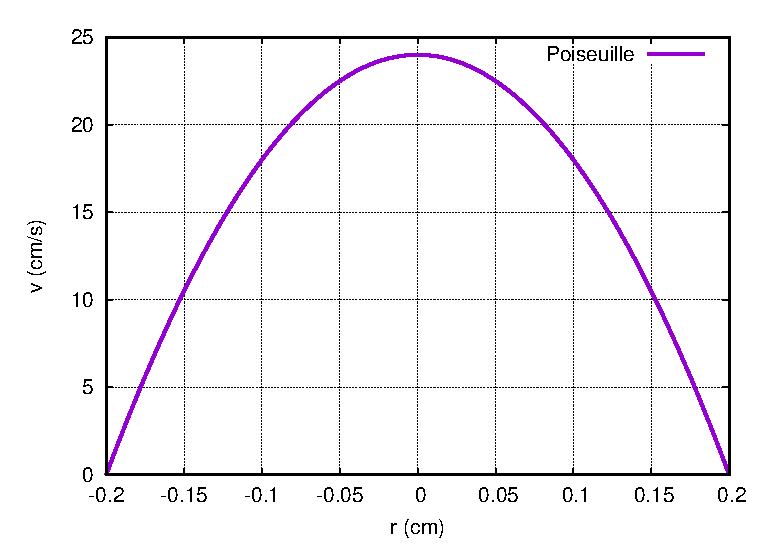
\includegraphics[width=0.6\textwidth]{figuras_4/pois.eps}
\caption{Definición analítica del flujo de Poiseuille para el caso considerado}
\label{fig:pois}
\end{figure}
\subsection{Aplicación hemodinámica}
\label{sec:aplicacion}
Consideraremos una aplicación al flujo sanguíneo, para una arteria de sección circular y diámetro $0.4$ cm, representativa de una carótida humana.
Las propiedades de la sangre se tomarán como densidad $\rho=1.06$ g/cm$^{3}$, viscosidad cinemática $\eta=0.04$ P (poise).
Se supone un flujo con una velocidad media $\bar v=12$ cm/s.
Consideraremos una longitud de la arteria $L=2$ cm, con una pérdida de presión a lo largo de la misma $\Delta p=192$ dyn/cm$^{2}$.
(Nota: Todas las magnitudes físicas se expresan en el sistema cgs --- centímetro, gramo, segundo.)
Para estos datos el perfil de velocidades de Poiseuille definido por la ecuación \eqref{eq:pois-vr} se representa en la fig.~\ref{fig:pois}.
La velocidad máxima vale $v_\text{max}=24$ cm/s, mientras que la velocidad media es $\bar v=12$ cm/s.
El número de Reynolds que corresponde al flujo es
\begin{equation*}
	\mathrm{Re} = \frac{\rho v D}{\eta} \approx 120
\end{equation*}
(siendo $D=2R$), lo que corresponde a una situación de flujo laminar.
En este caso el número de Womersley vale
\begin{equation}
	\alpha=R\sqrt{\frac{\omega\rho}{\eta}} = 2.79
\end{equation}
que al ser mayor que 1 indica que en rigor no sería esperable el desarrollo de un flujo de Poiseuiile debido a la frecuencia de las pulsaciones.

El fluido se supondrá prácticamente incompresible, para lo cual en las simulaciones numéricas se tomará un módulo de compresibilidad volumétrica elevado, $K=1\times 10^{7}$ dyn/cm$^{2}$.

\section{CFD en tubo recto}
\label{sec:tuborecto}

\subsection{Geometría, malla y material}

Se abre el programa \emph{FEBio Studio}, y al crear un nuevo modelo se selecciona un problema de \emph{Fluid Mechanics} (fig. \ref{fig:pre-00}).
\begin{figure}[!htp]
\centering
\begin{subfigure}[b]{0.30\textwidth}
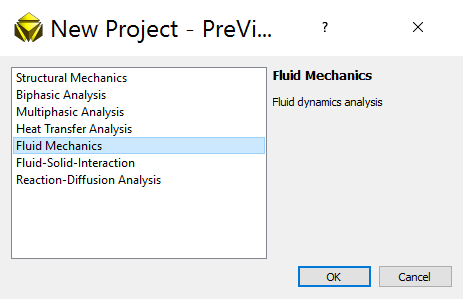
\includegraphics[width=\linewidth]{figuras_4/00_pre_newproject.png}
\caption{Apertura de Preview}
\label{fig:pre-00}
\end{subfigure}
\begin{subfigure}[b]{0.30\textwidth}
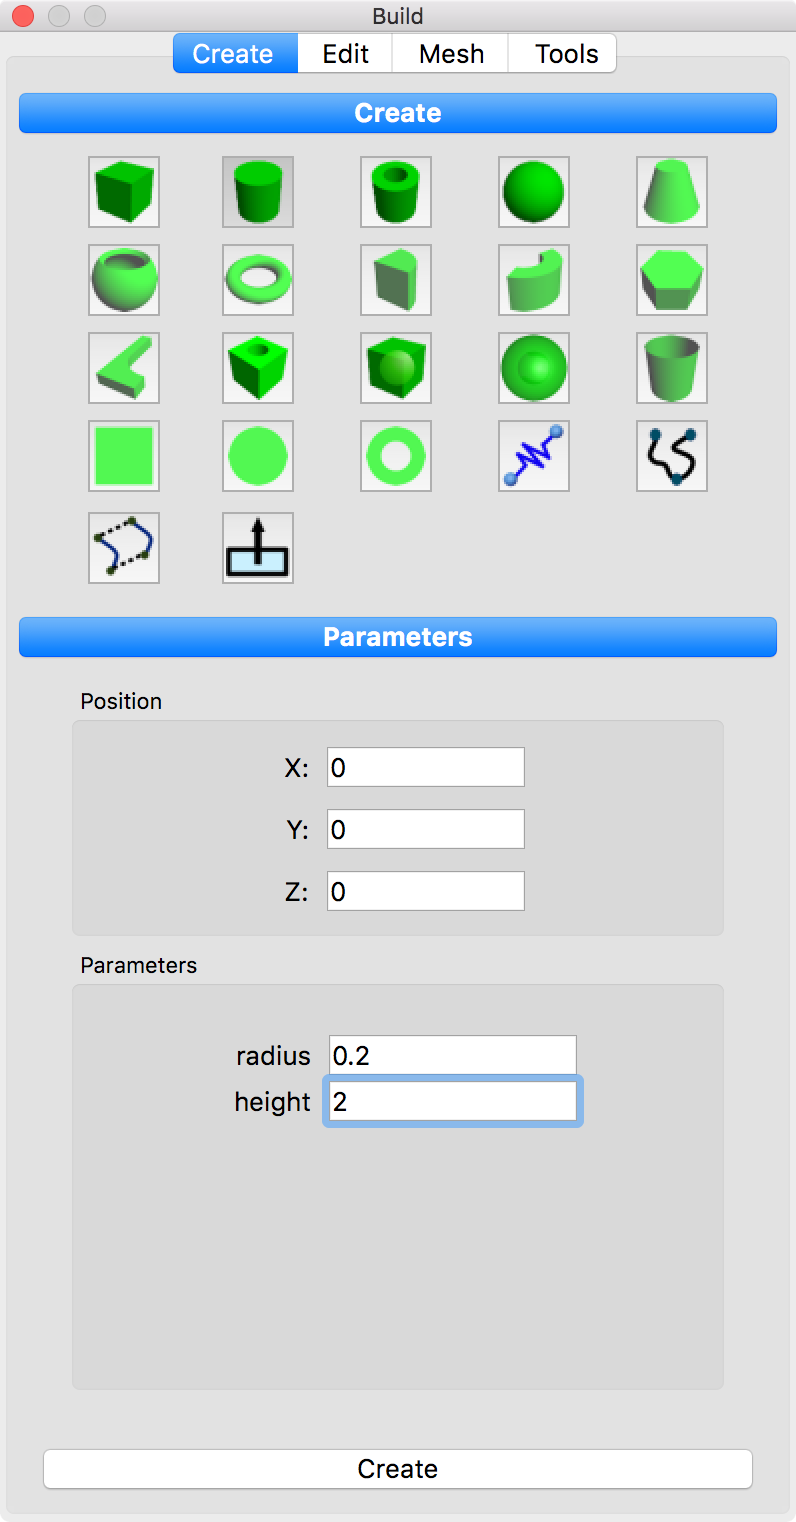
\includegraphics[width=\linewidth]{figuras_4/01_pre_create.png}
\caption{Geometría del cilindro}
\label{fig:pre-01-1}
\end{subfigure}
\begin{subfigure}[b]{0.30\textwidth}
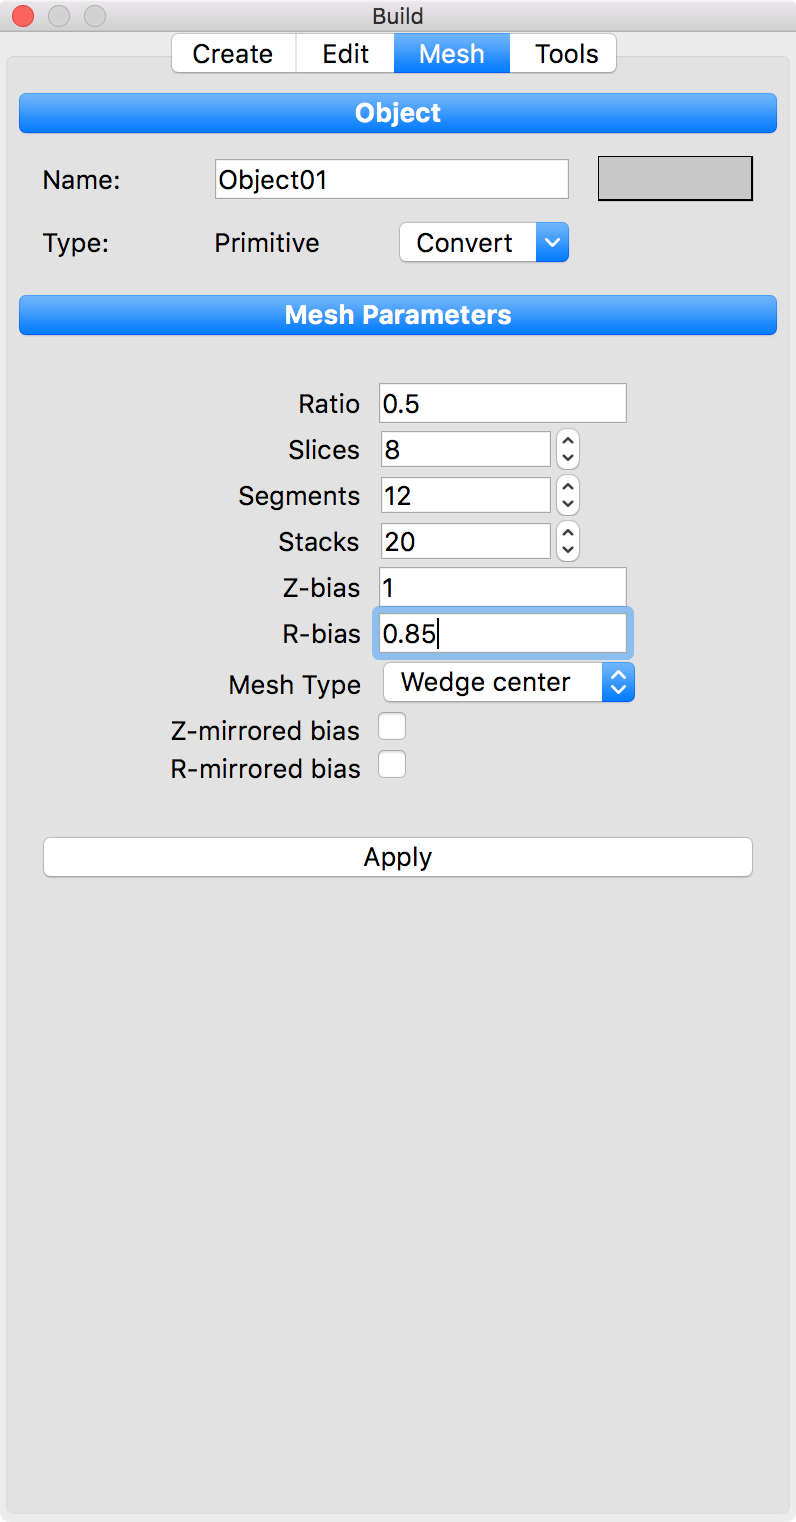
\includegraphics[width=\linewidth]{figuras_4/01_pre_mesh.png}
\caption{Malla del cilindro}
\label{fig:pre-01-2}
\end{subfigure}
\caption{Apertura de Preview y creación de geometría y malla}
\label{fig:pre-00-01}
\end{figure}
A continuación, en el módulo \emph{Build} se crea un objeto cilíndrico con las dimensiones anteriormente indicadas (fig. \ref{fig:pre-01-1}) y una malla como se define en la fig. \ref{fig:pre-01-2}.
El parámetro \emph{R-bias} sirve para hacer la malla más fina cerca del borde del tubo, donde el gradiente de velocidades es mayor.

El siguiente paso es crear el material, definir sus propiedades y asignarlo a la parte del modelo creada anteriormente, fig.~\ref{fig:pre-02}.
Para ello se activa la selección de partes en la barra superior, se activa la parte con el ratón, y se agrega para el material definido en el recuadro inferior del mismo.
Las propiedades del fluido que se han empleado son las definidas arriba en la sección \ref{sec:aplicacion}.
\begin{figure}[!htp]
\centering
\begin{subfigure}[b]{0.29\textwidth}
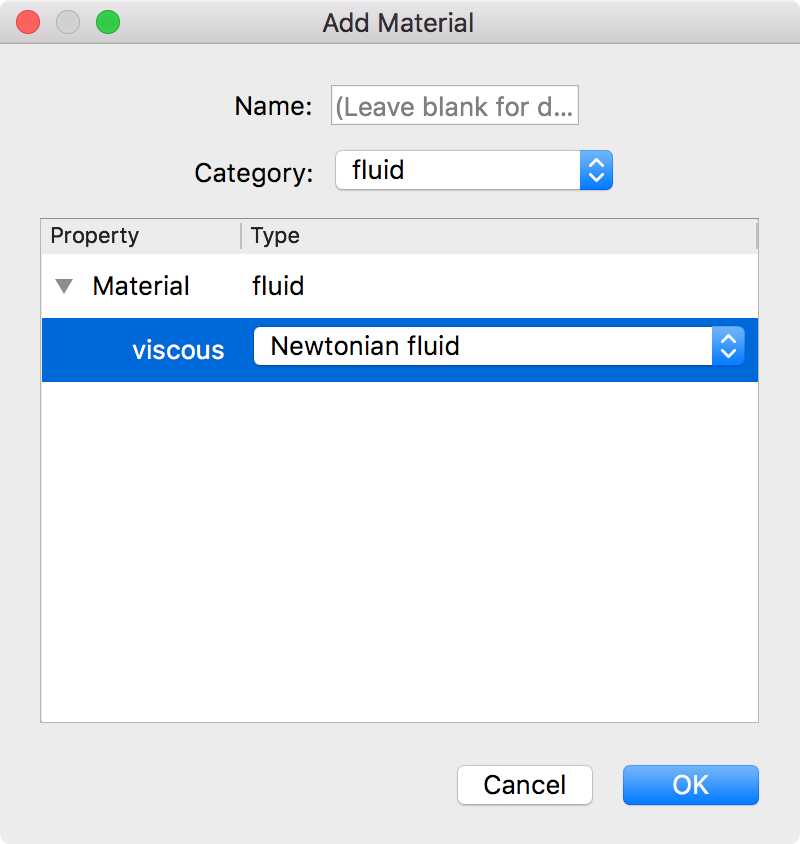
\includegraphics[width=\linewidth]{figuras_4/02_pre_mat-fluid-1.png}
\caption{Material: tipo fluido, viscosidad Newtoniana}
\label{fig:pre-02-a}
\end{subfigure}
\begin{subfigure}[b]{0.50\textwidth}
\centering
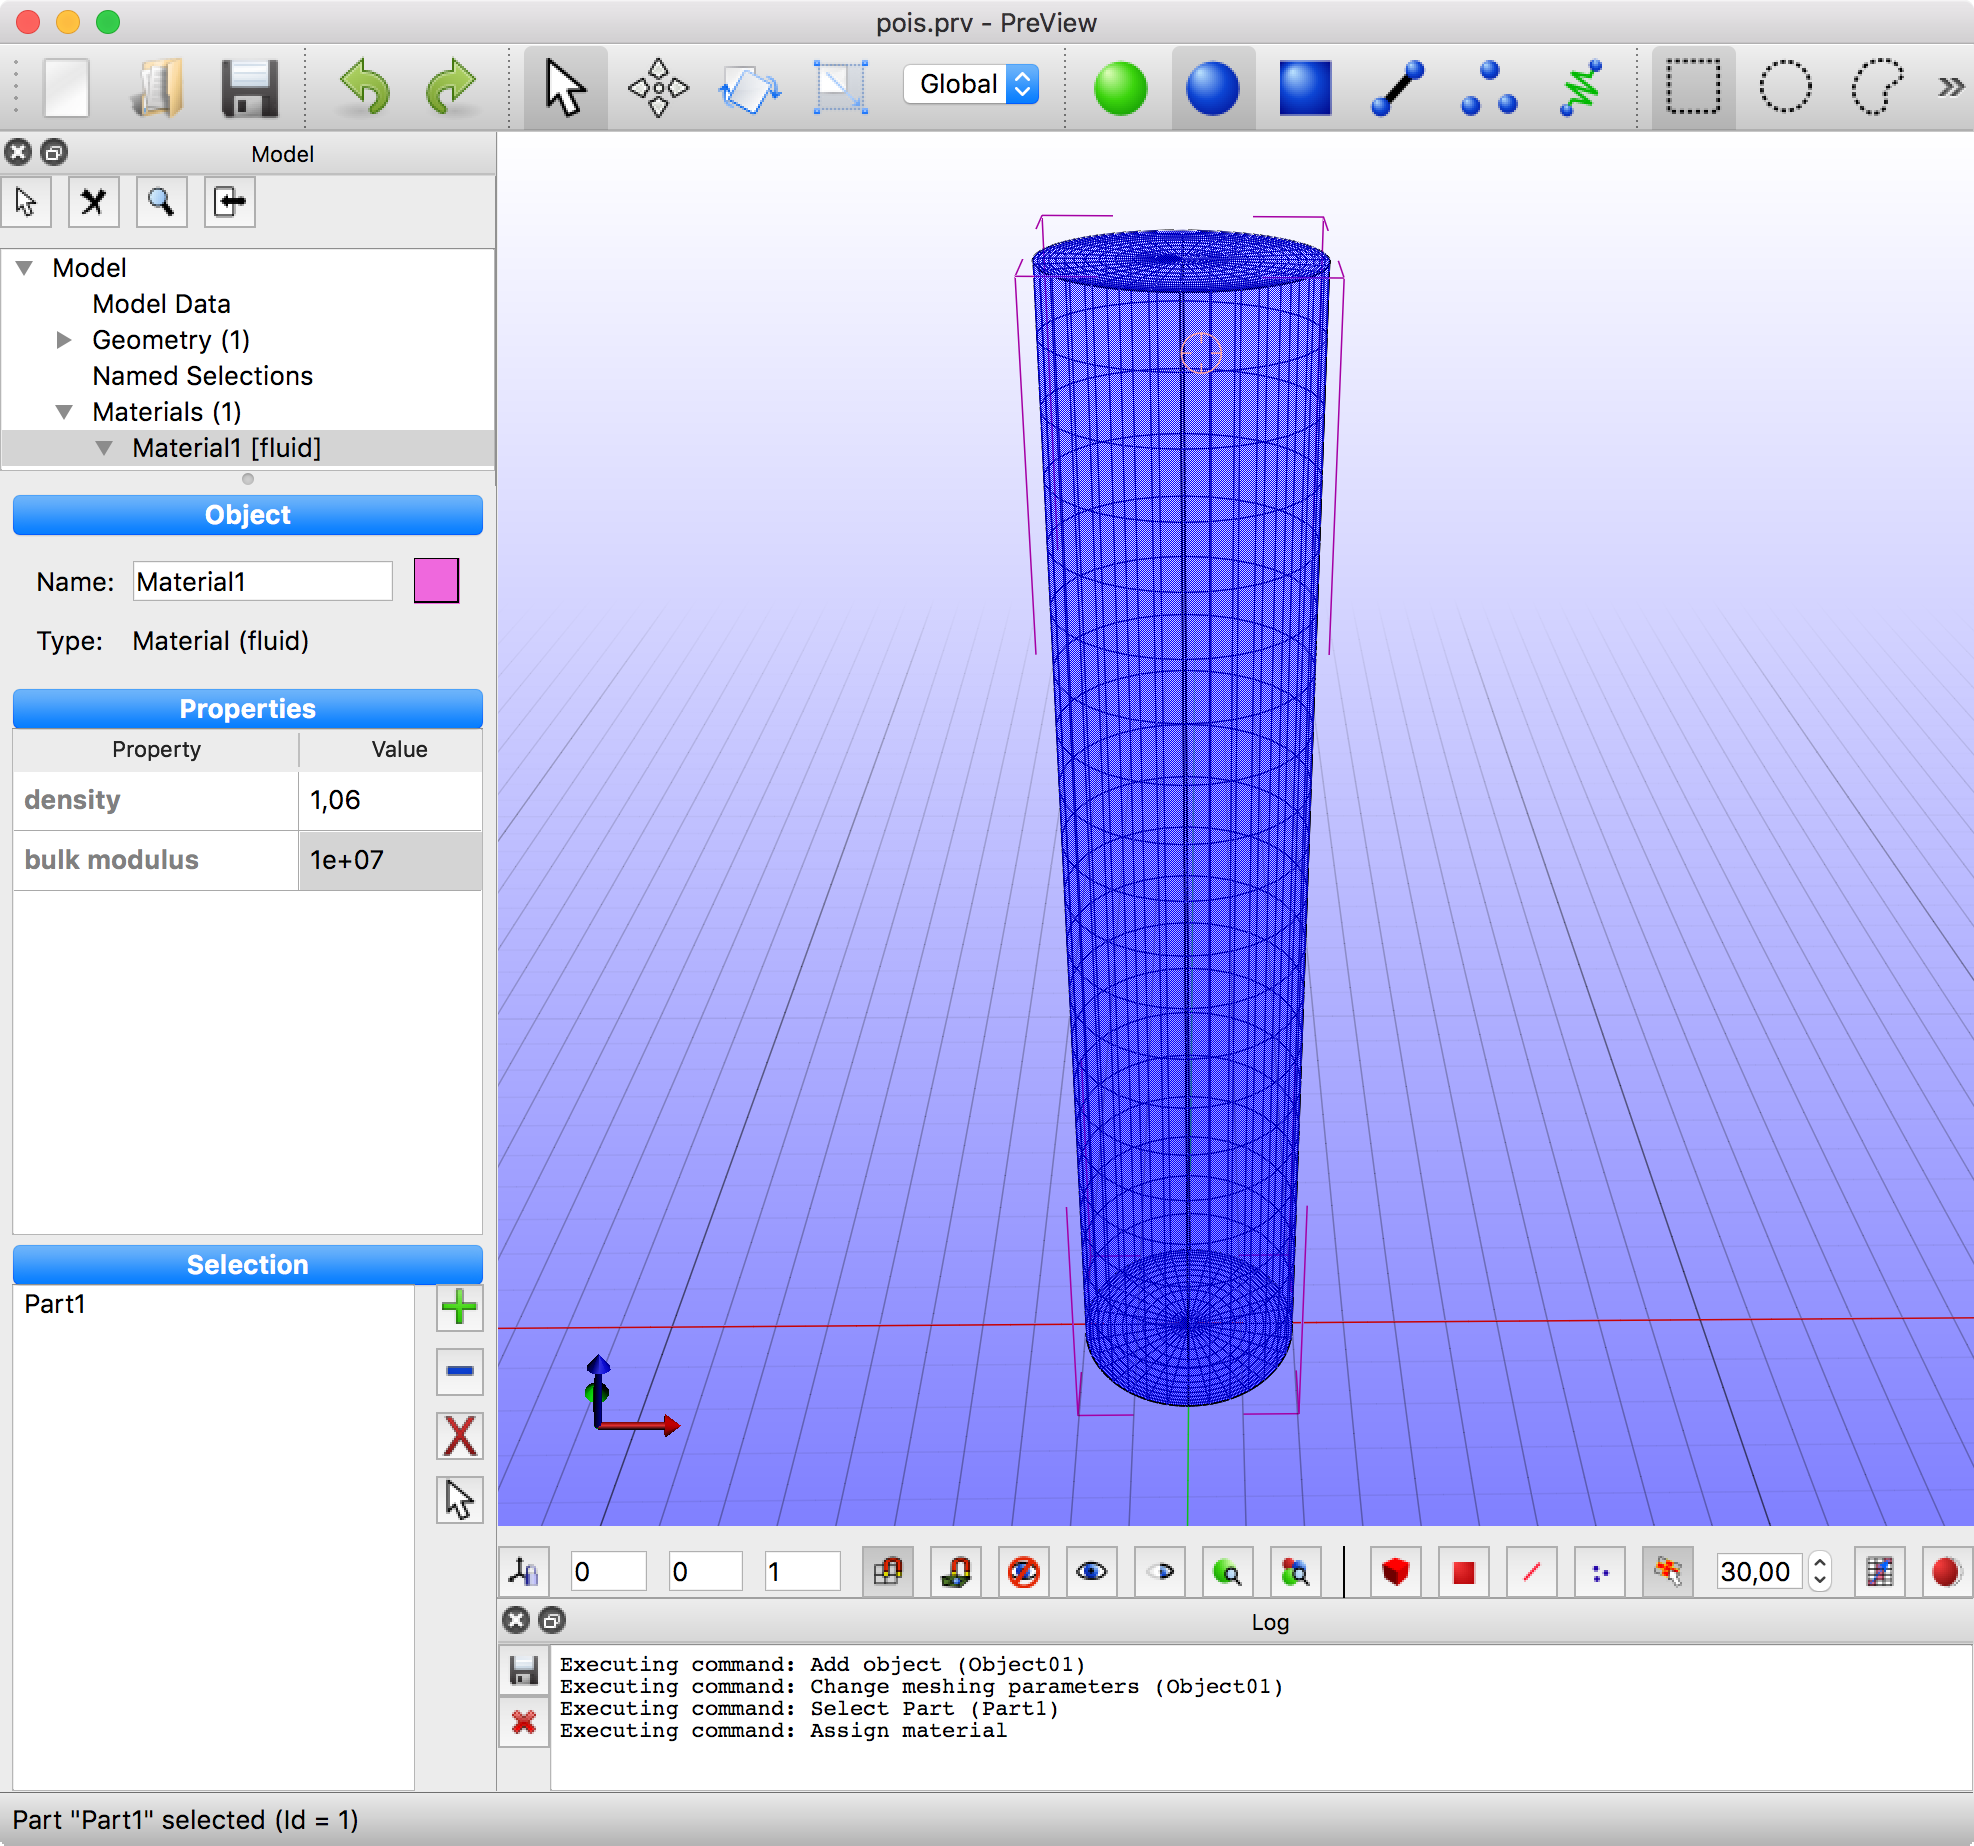
\includegraphics[width=\linewidth]{figuras_4/02_pre_mat-fluid-2.png}
\caption{Asignación del material y propiedades básicas del fluido}
\label{fig:pre-02-b}
\end{subfigure}
\begin{subfigure}[b]{0.19\textwidth}
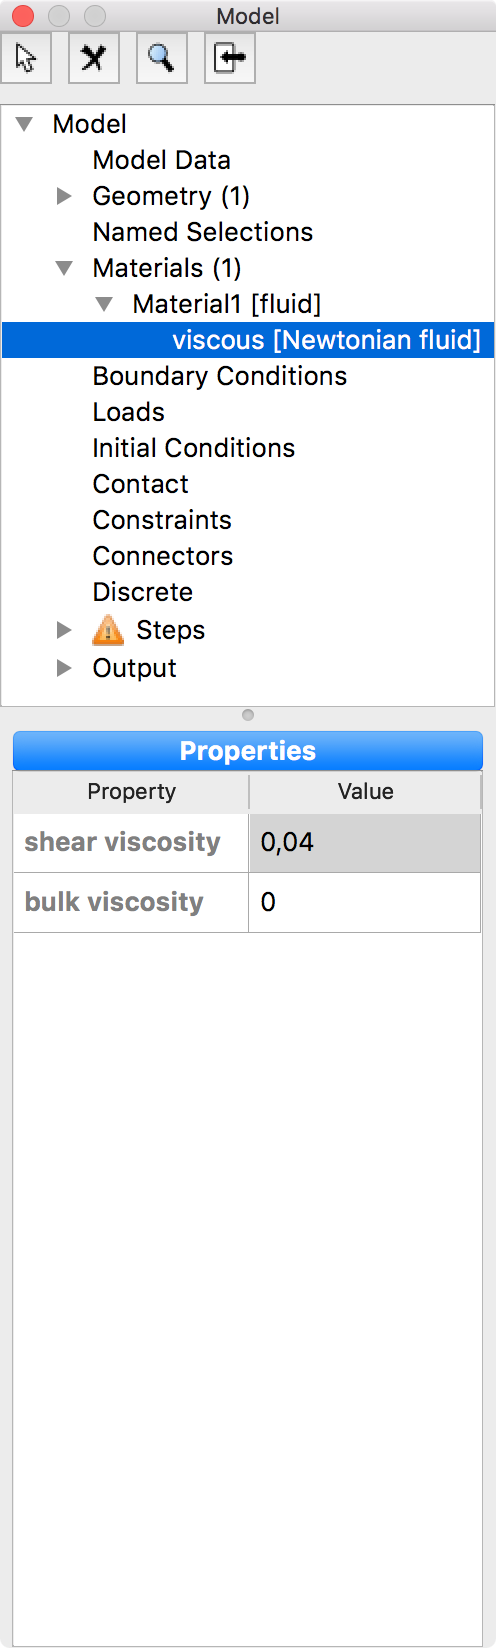
\includegraphics[width=\linewidth]{figuras_4/02_pre_mat-fluid-3.png}
\caption{Propiedades viscosas del fluido}
\label{fig:pre-02-c}
\end{subfigure}
\caption{Definición del material fluido y asignación al modelo (seleccionando la parte)}
\label{fig:pre-02}
\end{figure}

\subsection{Condiciones de contorno y cargas}

En primer lugar se define la condición de contorno de velocidad nula en la superficie lateral del cilindro (formada por cuatro superficies individuales en el modelo de \emph{Preview}).
Se agrega una nueva condición de contorno, seleccionándola como de velocidad nula (fig.~\ref{fig:pre-03-a}), y se asigna a las superficies laterales del cilindro (fig.~\ref{fig:pre-03-b}).
\begin{figure}[!ht]
\centering
\begin{subfigure}[b]{0.20\textwidth}
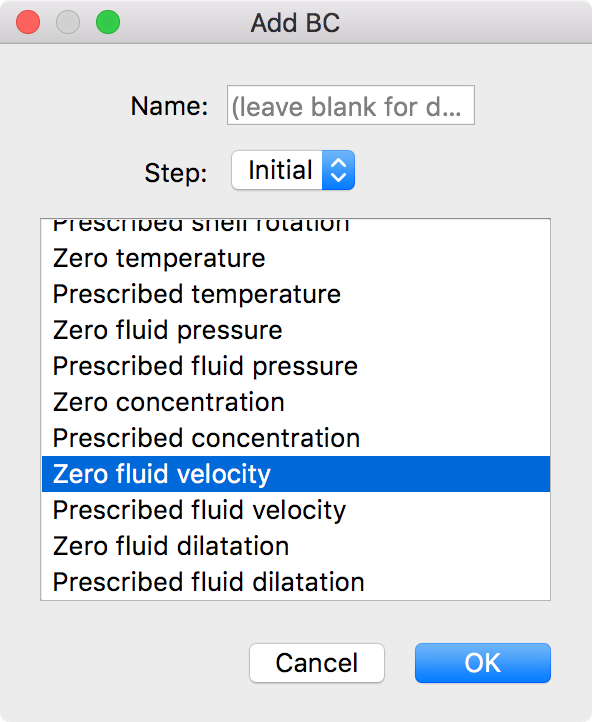
\includegraphics[width=\linewidth]{figuras_4/03_pre-bc-zfv-1.png}
\caption{CC: \emph{Zero fluid velocity}}
\label{fig:pre-03-a}
\end{subfigure}
\hfil
\begin{subfigure}[b]{0.48\textwidth}
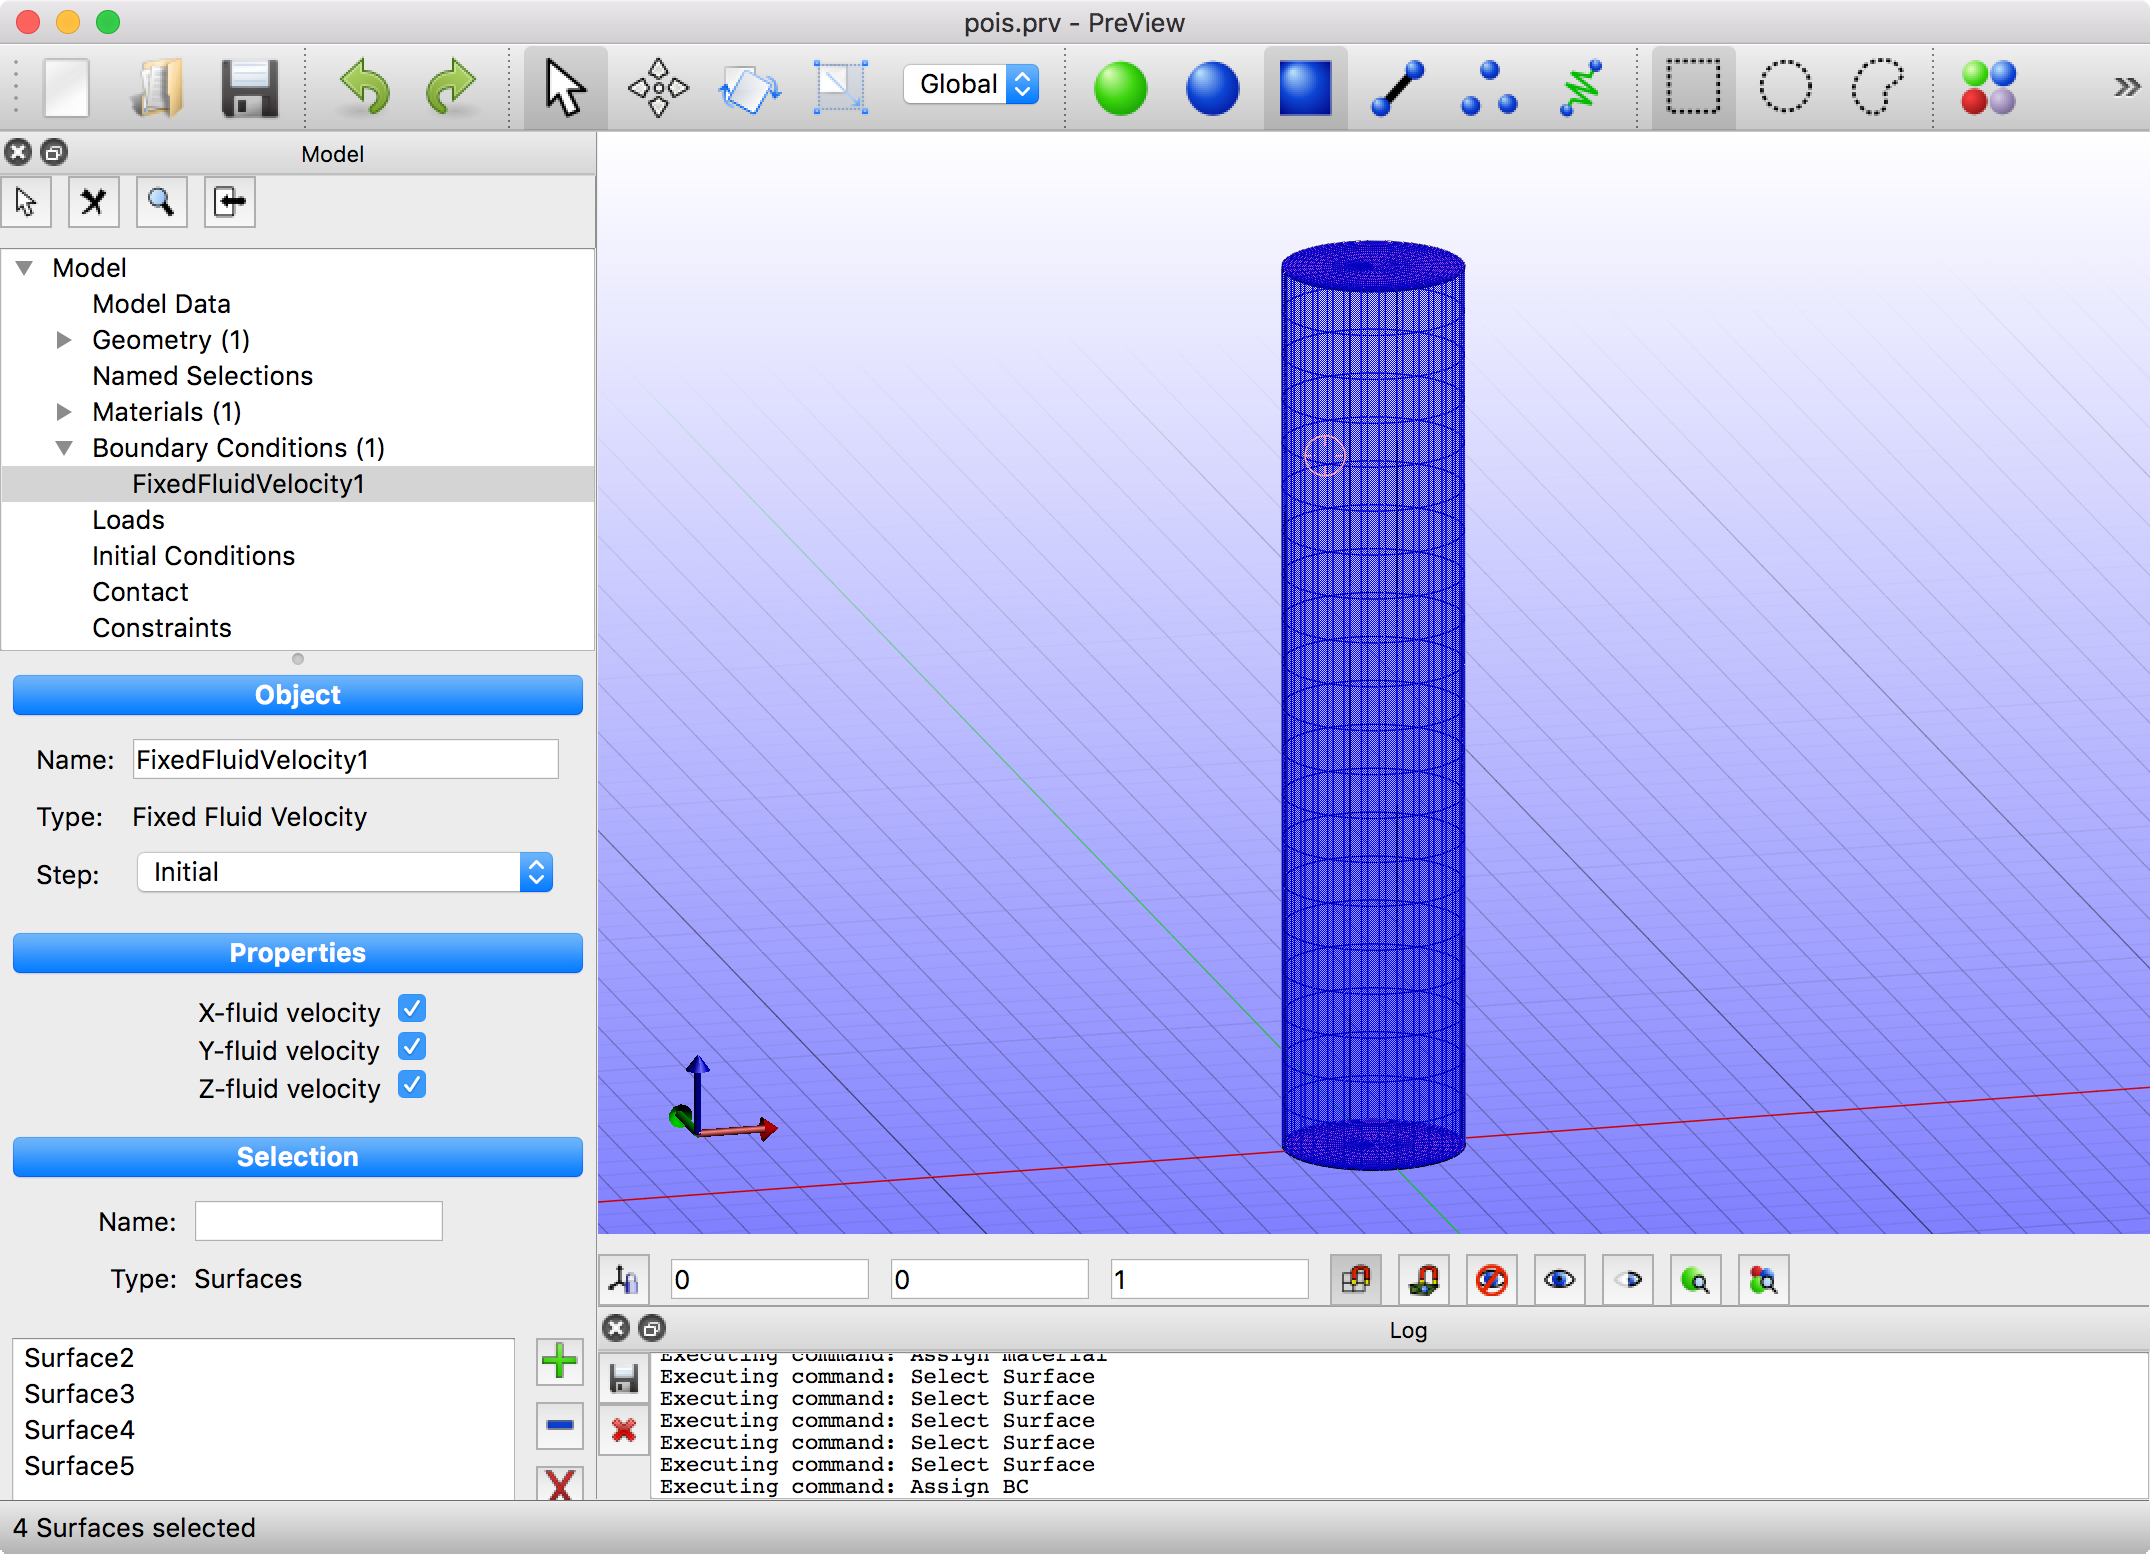
\includegraphics[width=\linewidth]{figuras_4/03_pre-bc-zfv-2.png}
\caption{Asignación a superficies laterales}
\label{fig:pre-03-b}
\end{subfigure}
\caption{Condición de contorno de velocidad nula en superficies laterales del cilindro}
\label{fig:pre-03-ab}
\end{figure}

A continuación definiremos las condiciones en las secciones inferior y superior del tubo, suponiendo que el flujo entra por la inferior y sale por la superior.
Se define la presión nula en la sección superior del tubo, lo que se realiza a partir de la variable \emph{fluid dilatation} ($e_{f}=J-1$) empleada por FEBiO.
Por ello la condición de contorno es \emph{Zero fluid dilatation} (fig.~\ref{fig:pre-04-a}) y se asigna a la superficie superior, de salida del flujo (fig.~\ref{fig:pre-04-b}).
\begin{figure}[!ht]
\centering
\begin{subfigure}[b]{0.20\textwidth}
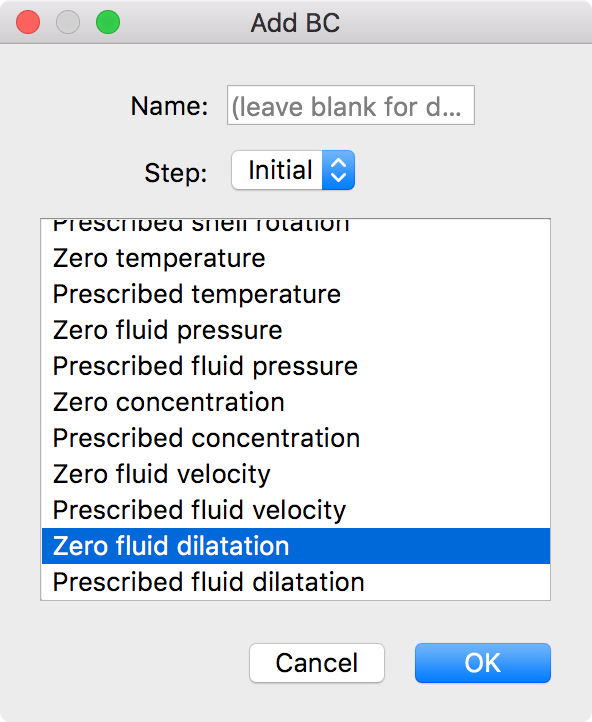
\includegraphics[width=\linewidth]{figuras_4/04_pre-bc-zfd-1.png}
\caption{CC: \emph{Zero fluid dilatation}}
\label{fig:pre-04-a}
\end{subfigure}
\hfil
\begin{subfigure}[b]{0.48\textwidth}
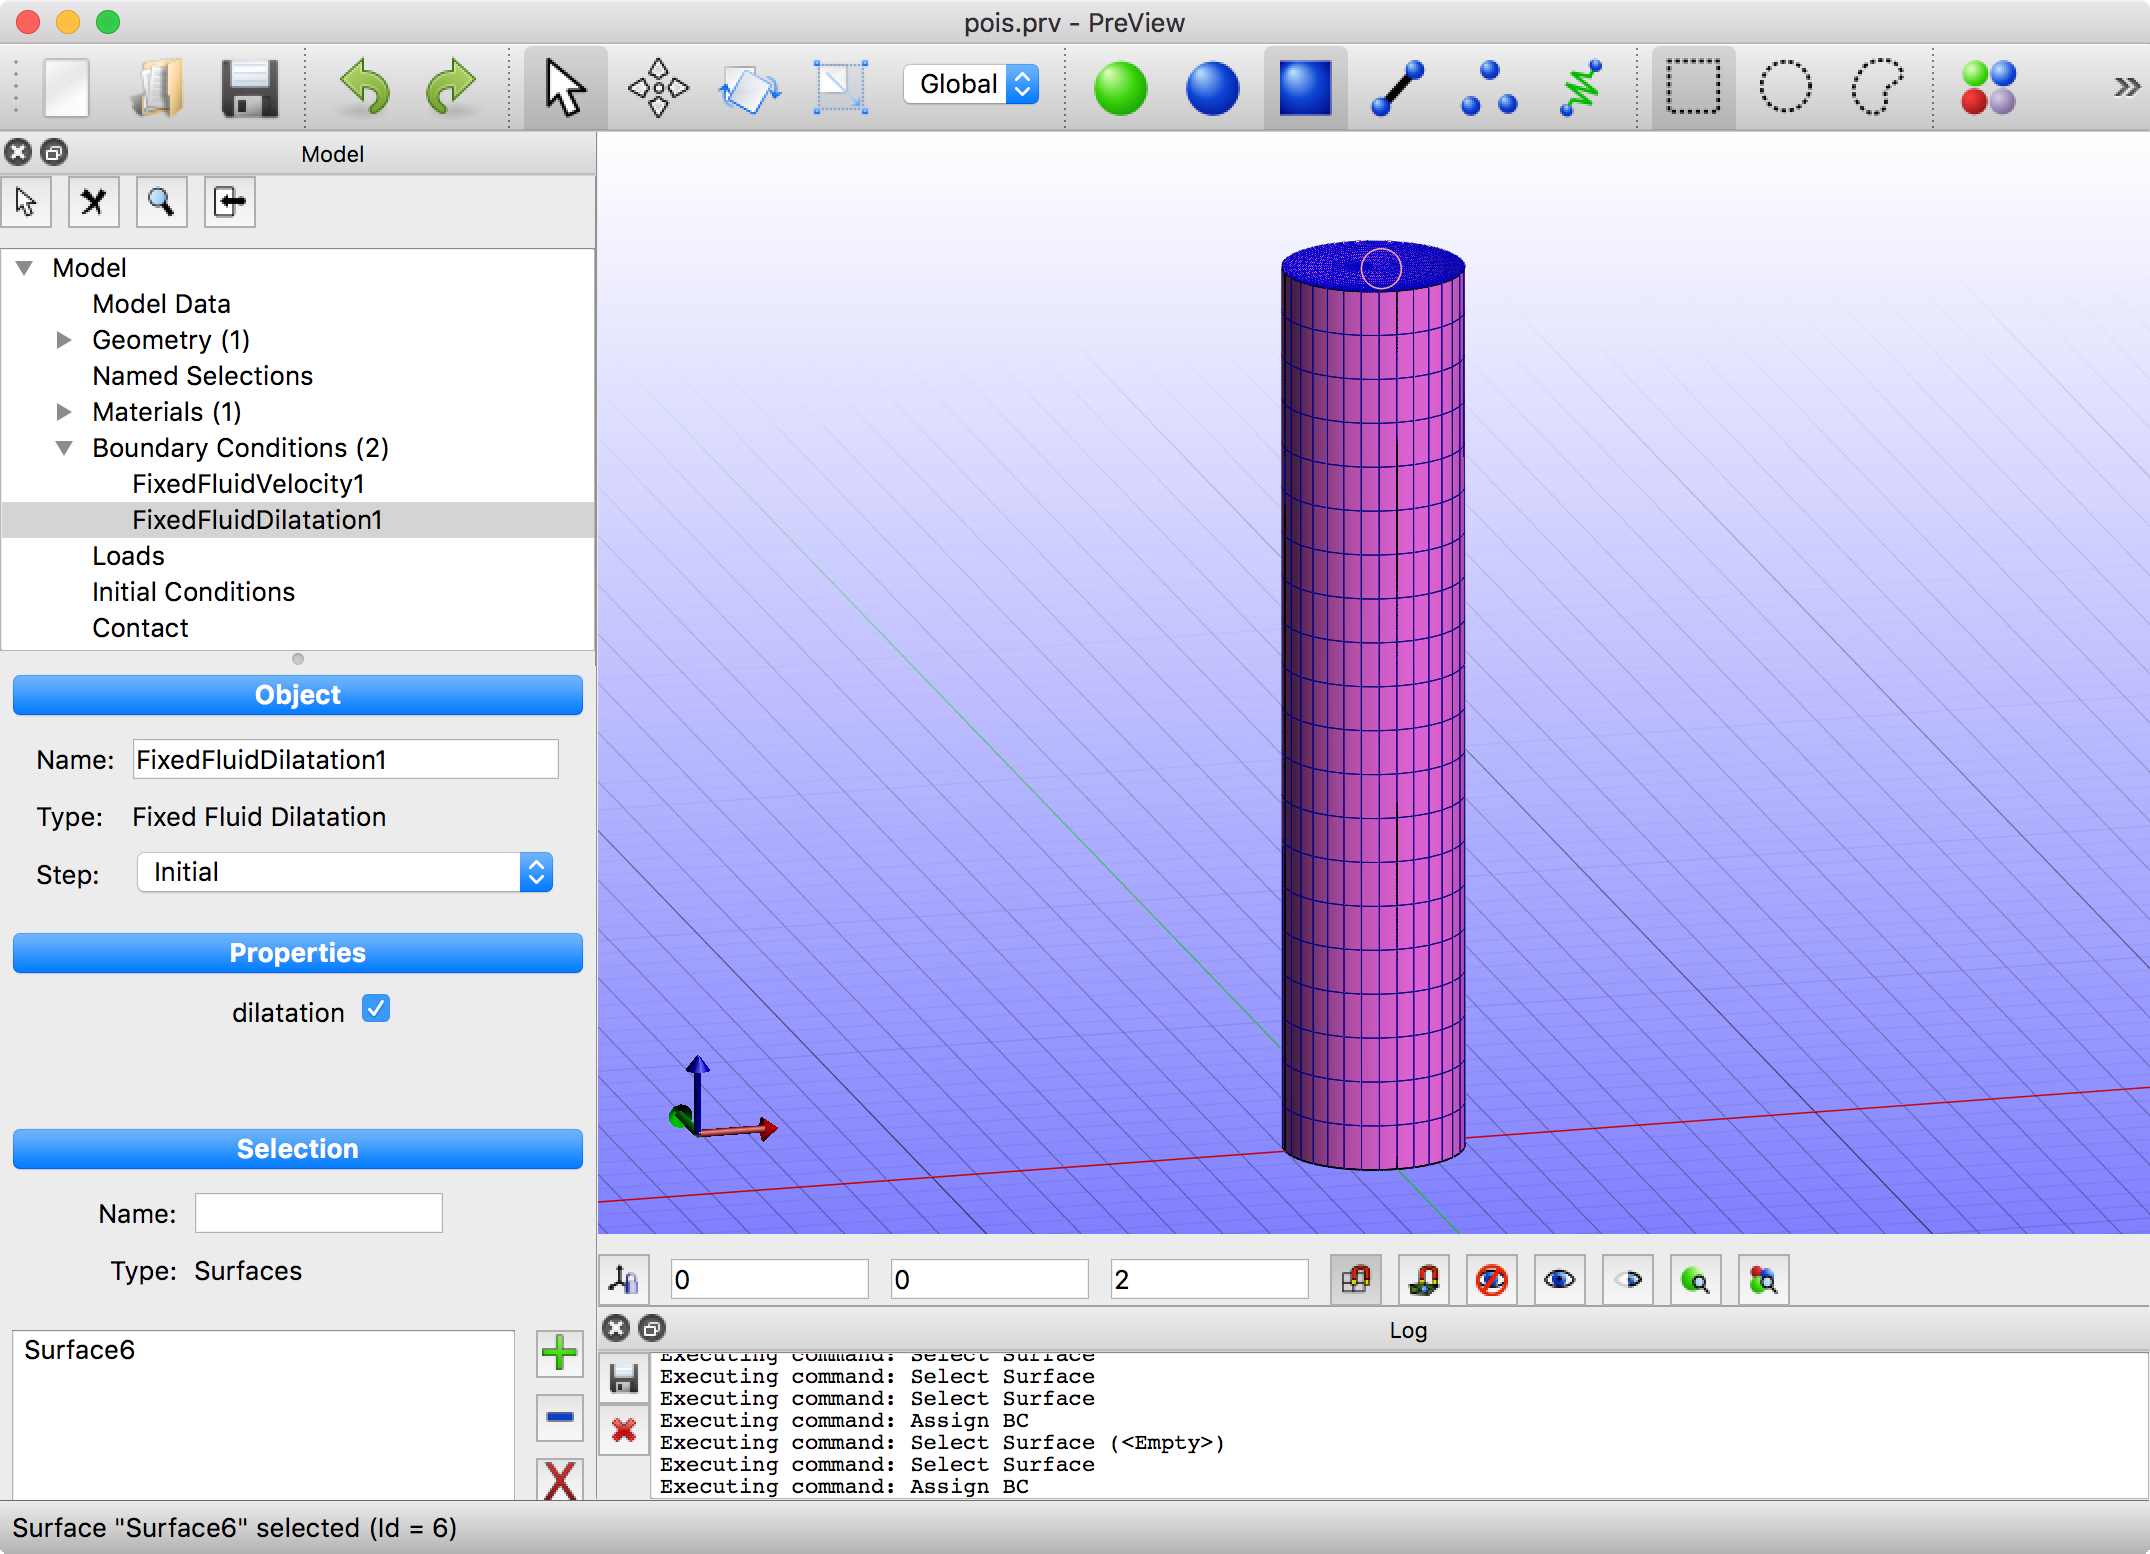
\includegraphics[width=\linewidth]{figuras_4/04_pre-bc-zfd-2.png}
\caption{Asignación a superficie superior}
\label{fig:pre-04-b}
\end{subfigure}
\caption{Condición de contorno de presión nula (a través de \emph{fluid dilatation}) en superficie superior del cilindro}
\label{fig:pre-04-ab}
\end{figure}

En la sección inferior, antes de definir la entrada del fluido, es necesario para evitar inestabilidades imponer en el borde de dicha sección una condición de presión nula \emph{Zero fluid dilatation}.
Para ello tendremos ciudado en primer lugar de activar la selección de bordes en los iconos de la barra superior, y a continuación seleccionar los cuatro segmentos de la circunferencia exterior de la base (fig. \ref{fig:pre-04-c})
\begin{figure}[!ht]
\centering
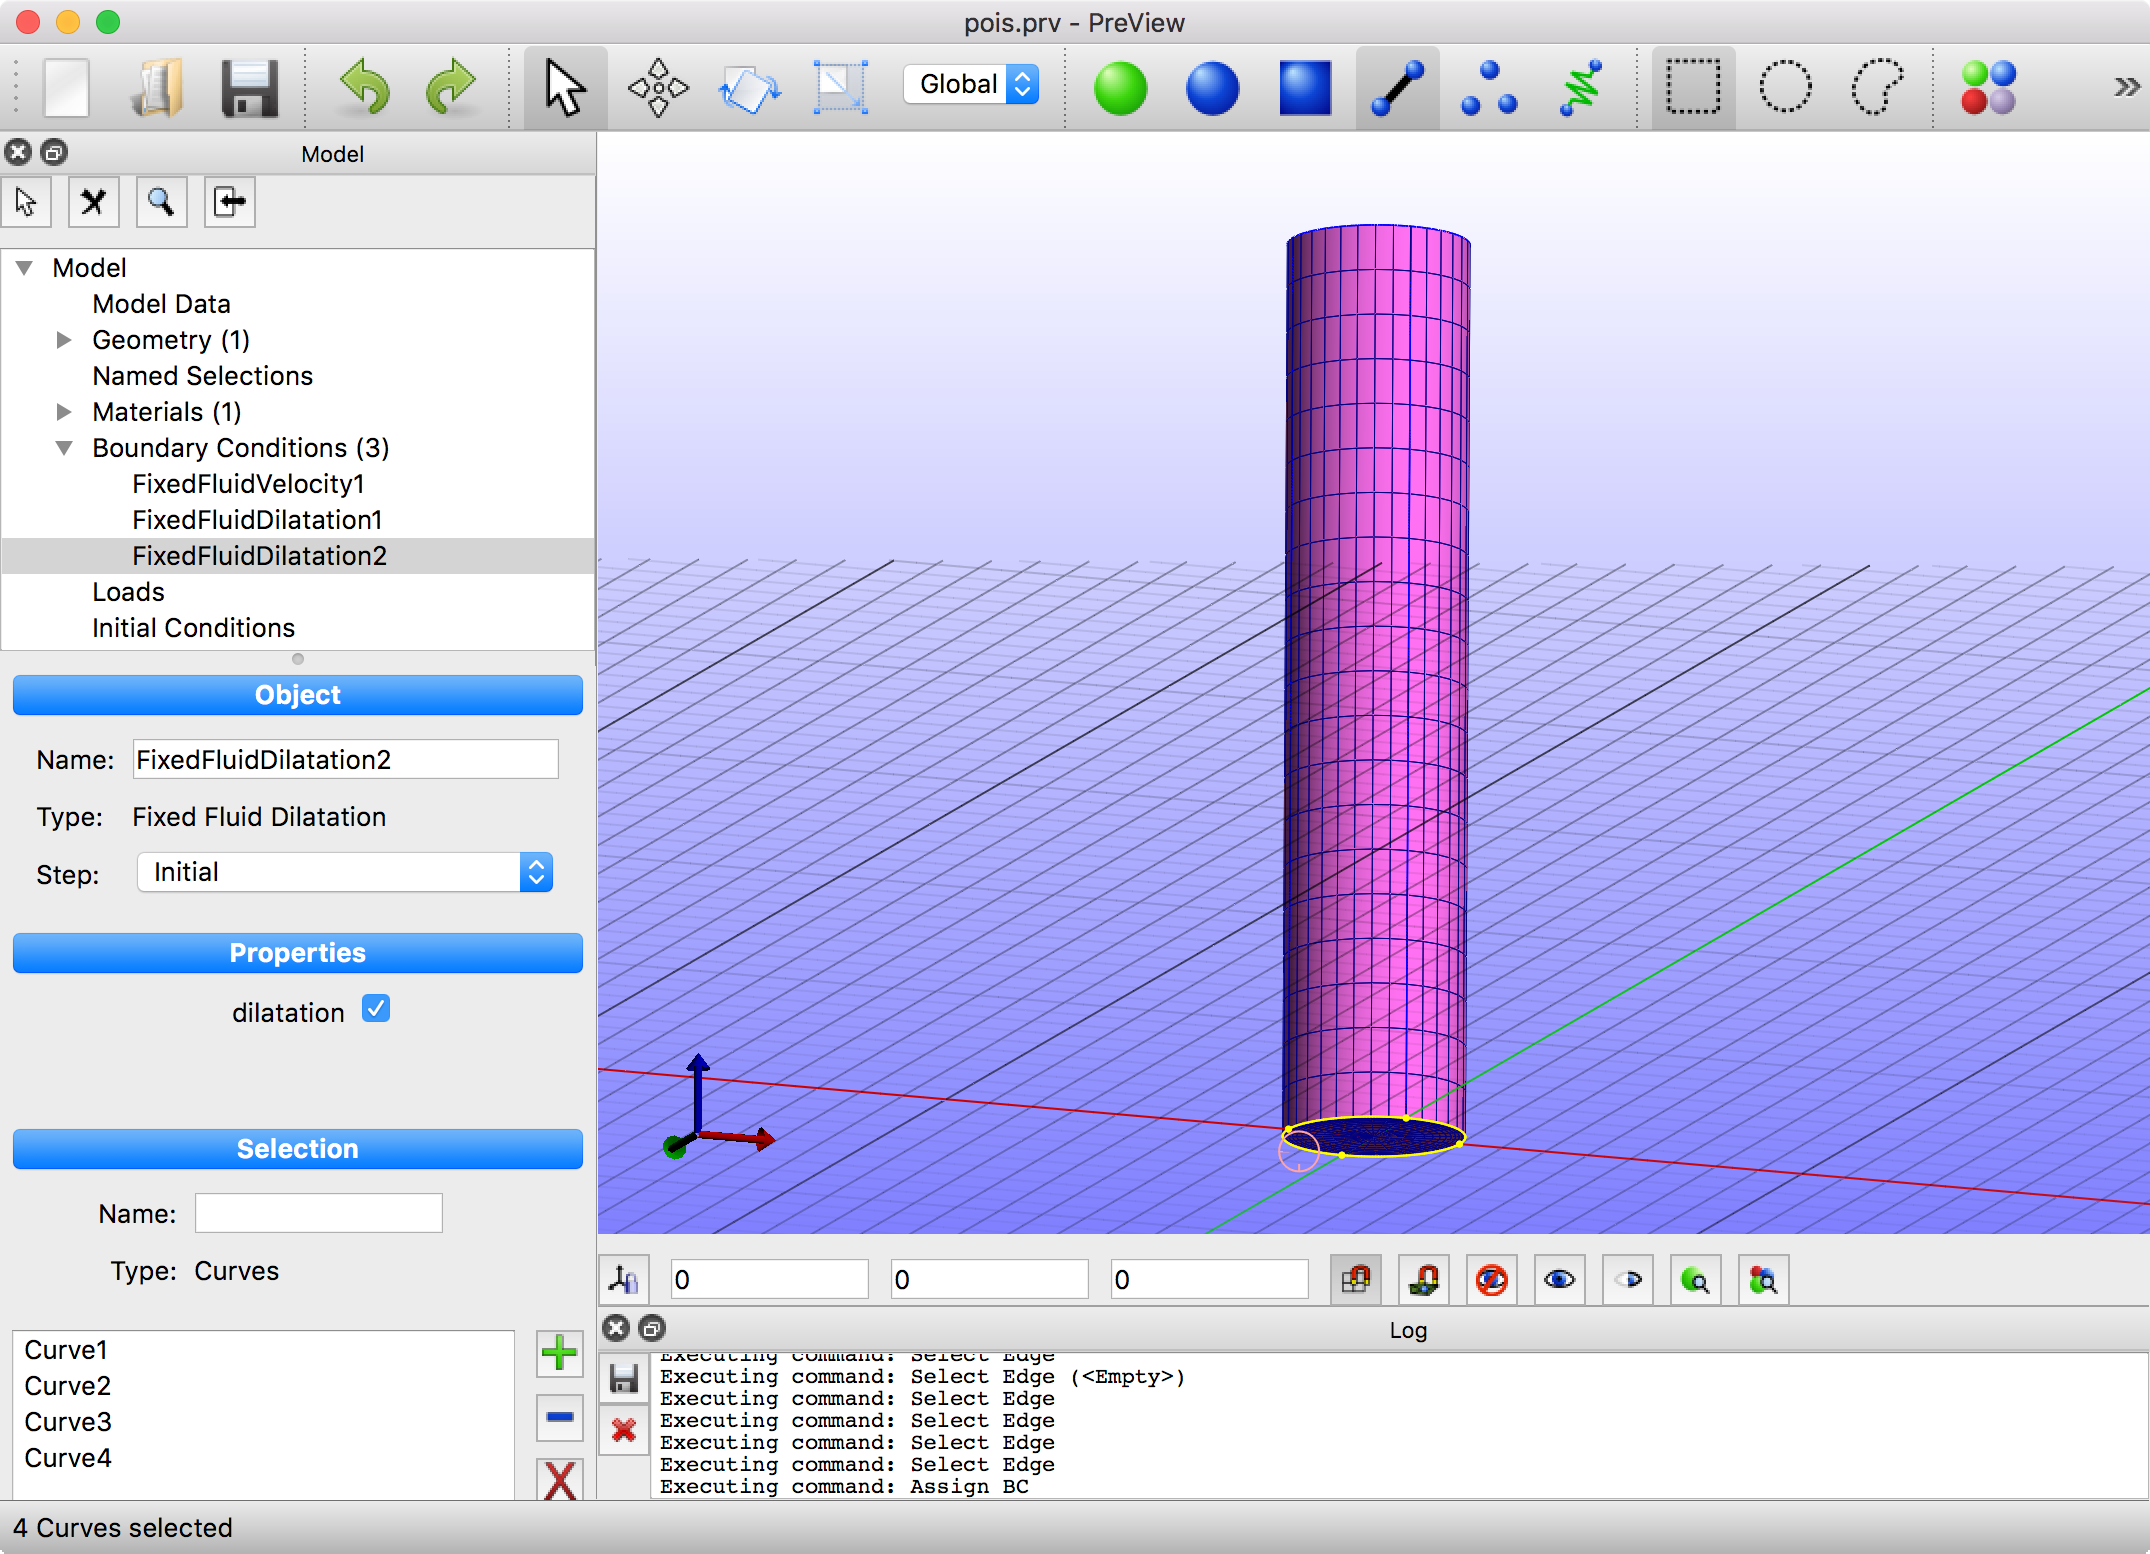
\includegraphics[width=0.48\linewidth]{figuras_4/04_pre-bc-zfd-3.png}
\caption{Condición de contorno de presión nula (a través de \emph{fluid dilatation}) en el borde de la base inferior}
\label{fig:pre-04-c}
\end{figure}

Por último se define la entrada de fluido en la cara de la sección inferior mediante \emph{Add surface load} / \emph{Fluid normal velocity} (fig.~\ref{fig:pre-05-a}) que aplicaremos a la cara de la base inferior (fig.~\ref{fig:pre-05-c}).
Por otra parte queremos aplicar esta carga durante un periodo de tiempo de $1.5$ para lo cual definimos la curva de aplicación correspondiente modificando el valor por defecto de $(1.0, 1.0)$ a $(1.5, 1.0)$ (fig.~\ref{fig:pre-05-b}).
\begin{figure}[!ht]
\centering
\begin{subfigure}[b]{0.35\textwidth}
\centering
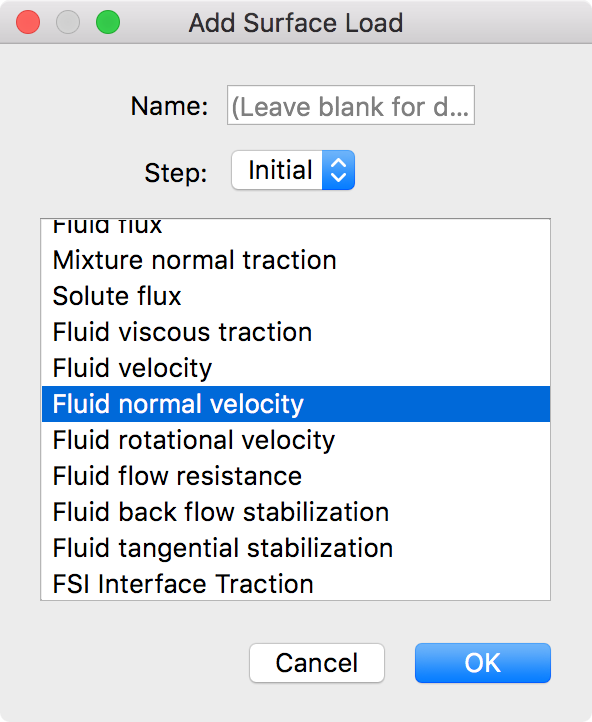
\includegraphics[width=0.6\linewidth]{figuras_4/05_pre_load-fnv-1.png}
\caption{Definir \emph{Fluid normal velocity}}
\label{fig:pre-05-a}
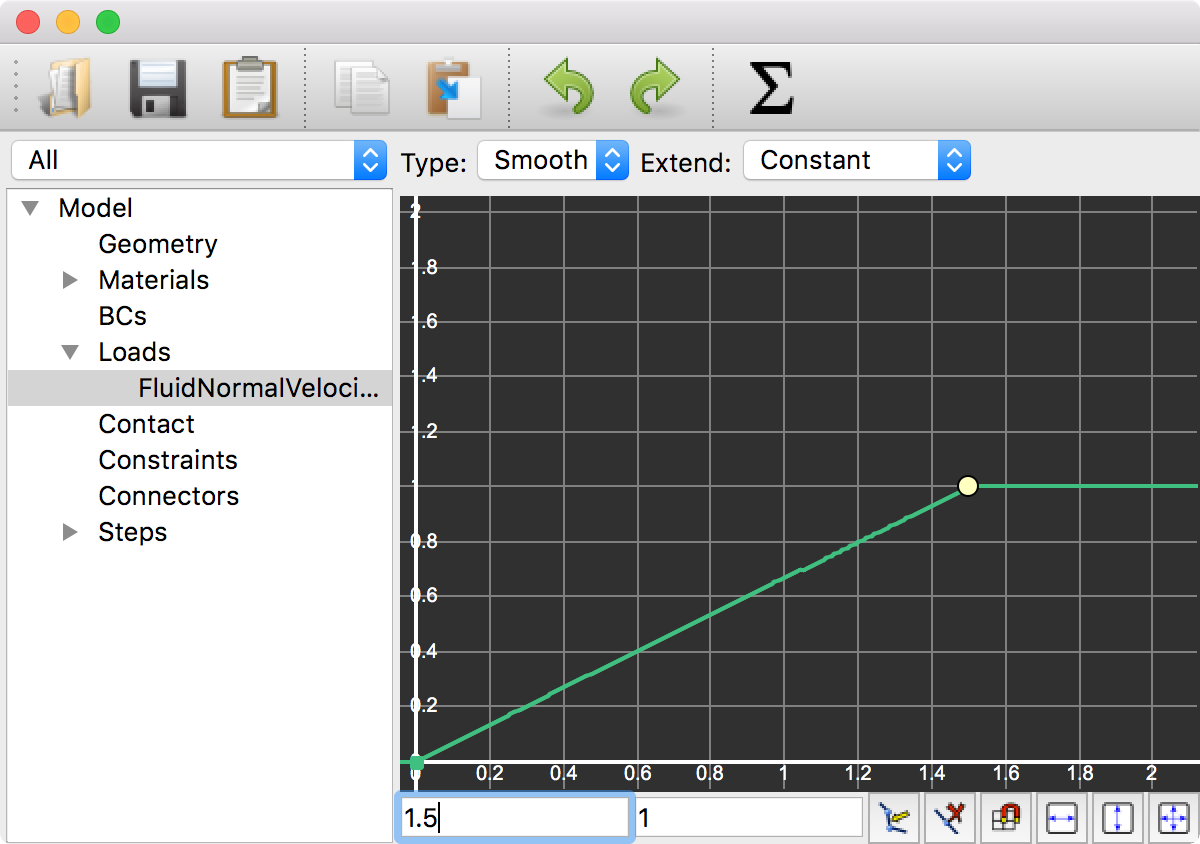
\includegraphics[width=\linewidth]{figuras_4/05_pre_load-fnv-3.png}
\caption{Curva de aplicación de la carga}
\label{fig:pre-05-b}
\end{subfigure}
\hfil
\begin{subfigure}[b]{0.55\textwidth}
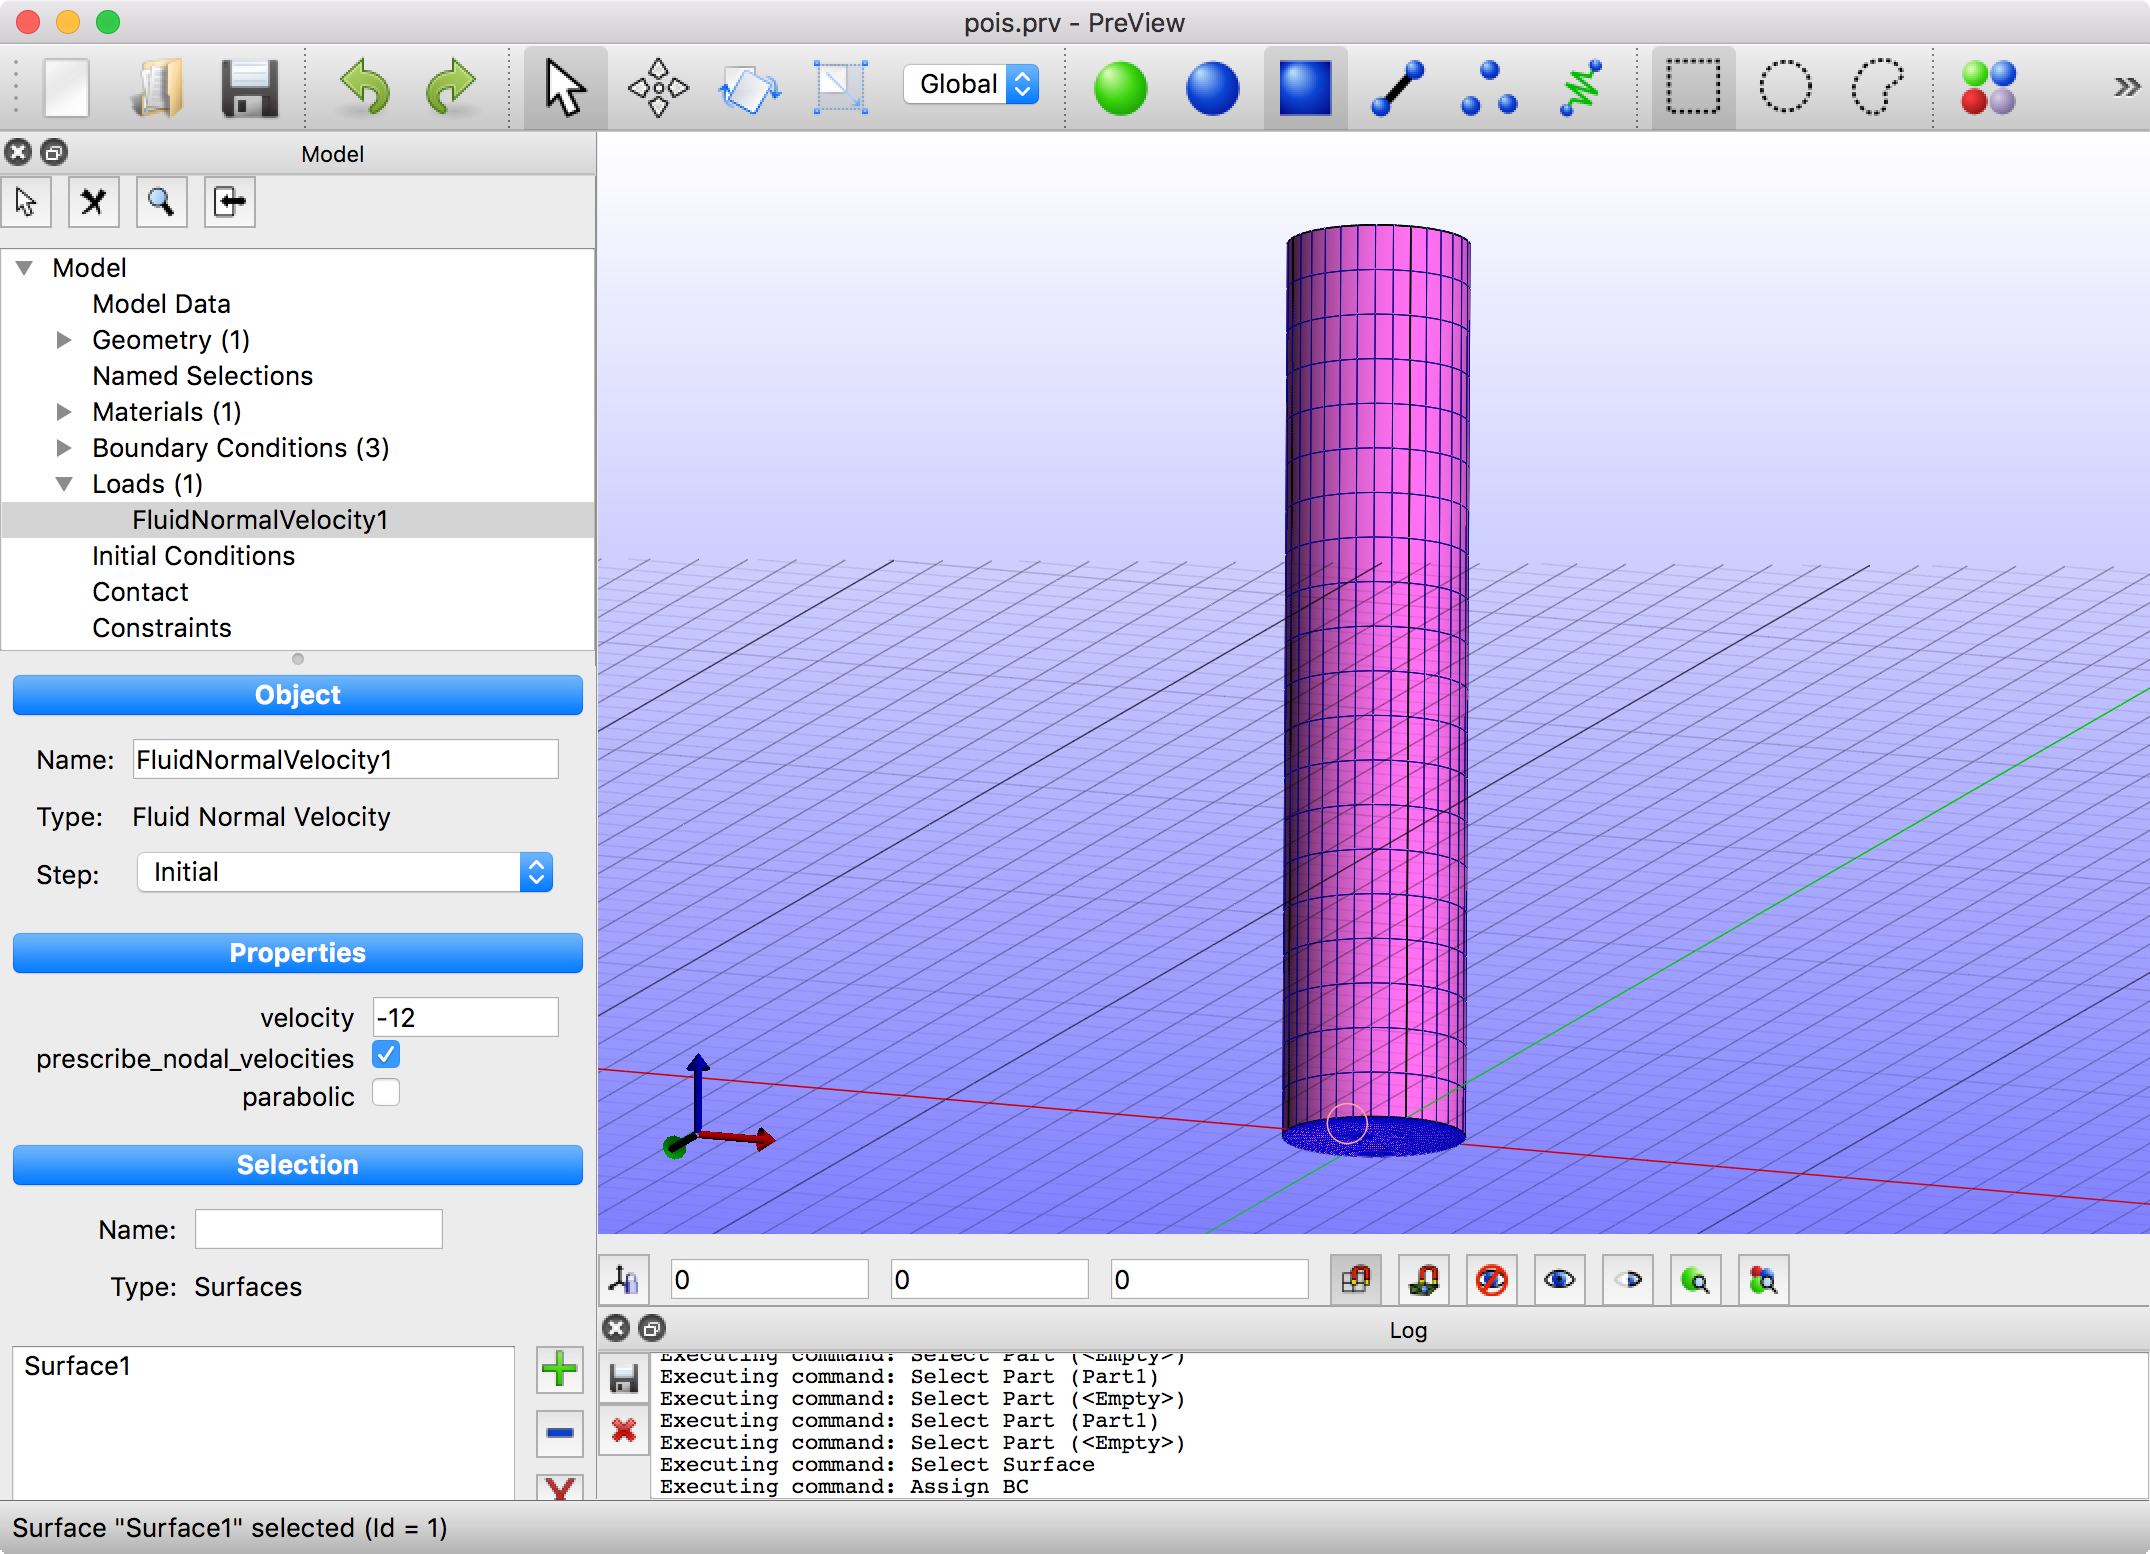
\includegraphics[width=\linewidth]{figuras_4/05_pre_load-fnv-2.png}
\caption{Asignación de flujo a superficie inferior}
\label{fig:pre-05-c}
\end{subfigure}
\caption{Definición de velocidad del fluido de entrada en la sección inferior del tubo}
\label{fig:pre-05}
\end{figure}
En un primer cálculo dejamos sin marcar la casilla \emph{parabolic} (fig.~\ref{fig:pre-05-c}), lo que equivale a que la velocidad se aplicará de manera uniforme en la superficie indicada.
Una vez completado este primer cálculo, lo repetiremos modificando solo este aspecto, es decir marcando la casilla \emph{parabolic}.

\subsection{Caso de cálculo}

Por último se agrega y define el \emph{Step} de cálculo, del tipo \emph{Fluid mechanics} (fig.~\ref{fig:pre-06-a}), modificando los siguientes parámetros respecto a los que aparecen por defecto (figs. \ref{fig:pre-06-b}, \ref{fig:pre-06-c}):
\begin{itemize}
	\item
	Número de pasos (\emph{Time steps}): 25 (tiempo de simulación $T=25\cdot 0.1=2.5$)
	\item
	Matriz no simétrica
	\item
	Método Quasi-Newton: \emph{Broyden}
	\item
	\emph{Residual tolerance}: $0.001$
	\item
	\emph{Spectral radius}: $\rho_{\infty}=0$
	\item
	\emph{Max reformations}: 3
	\item
	\emph{Max updates}: 50
	\item
	Dejar sin marcar las dos últimas casillas de \emph{Reform on diverge} / \emph{Reform each timestep}
\end{itemize}

\begin{figure}[!ht]
\centering
\begin{subfigure}[b]{0.225\textwidth}
\centering
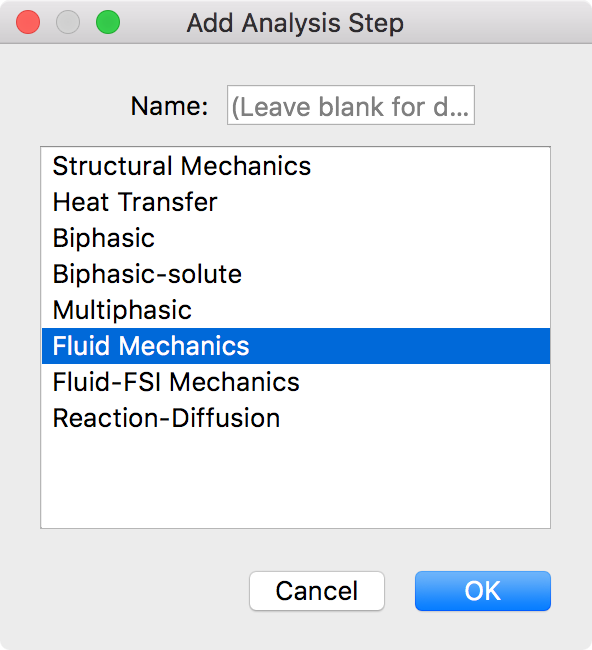
\includegraphics[width=\linewidth]{figuras_4/06_pre_step-0.png}
\caption{Crear \emph{Step} de cálculo del tipo \emph{Fluid Mechanics}}
\label{fig:pre-06-a}
\end{subfigure}
\hfil
\begin{subfigure}[b]{0.25\textwidth}
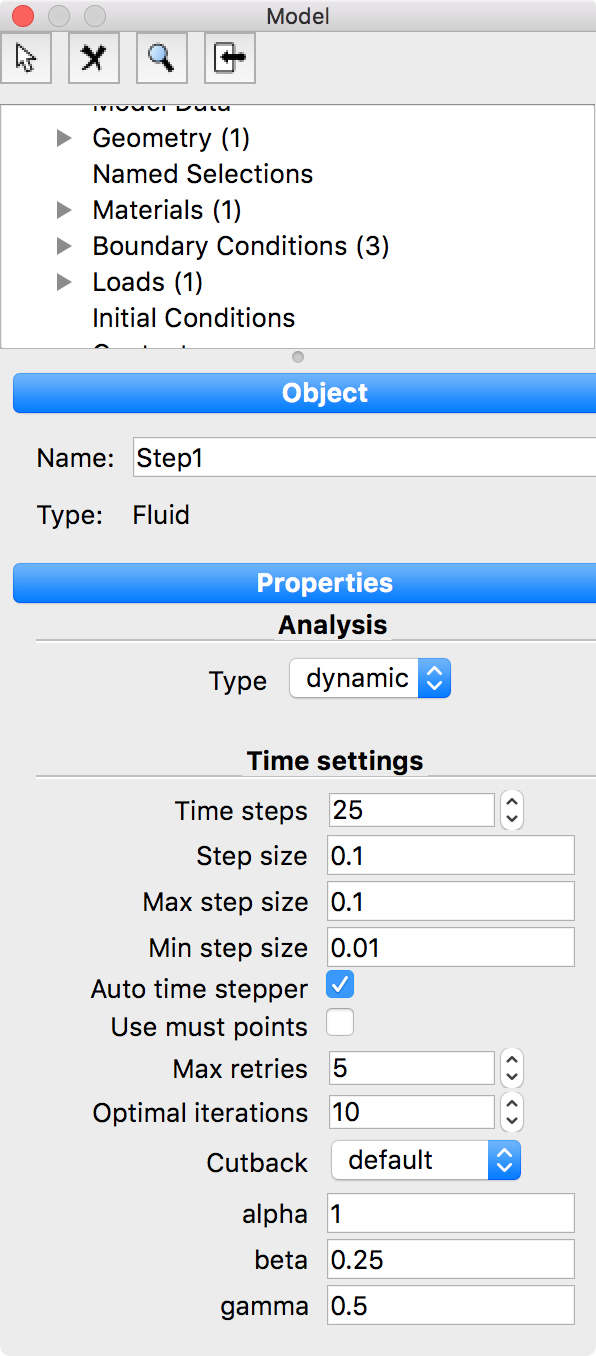
\includegraphics[width=\linewidth]{figuras_4/06_pre_step-1.png}
\caption{Parámetros del \emph{Step} (I)}
\label{fig:pre-06-b}
\end{subfigure}
\hfil
\begin{subfigure}[b]{0.25\textwidth}
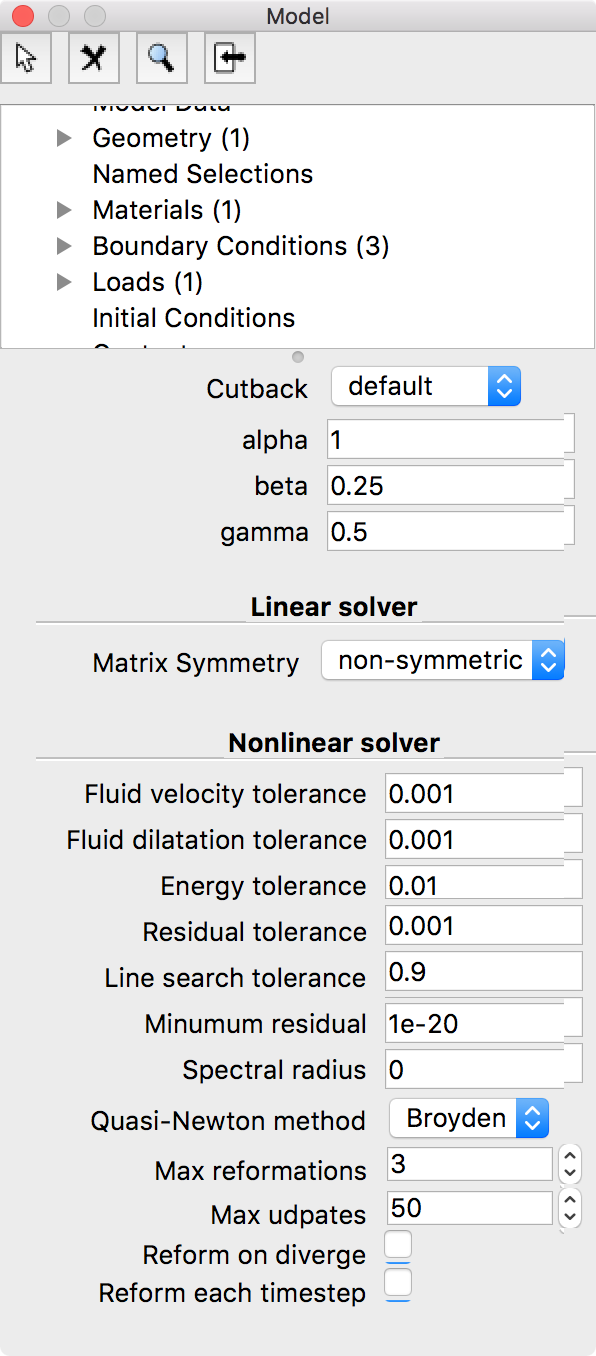
\includegraphics[width=\linewidth]{figuras_4/06_pre_step-2.png}
\caption{Parámetros del \emph{Step} (II)}
\label{fig:pre-06-c}
\end{subfigure}
\caption{Definición del \emph{Step} para el cálculo CFD y parámetros del mismo}
\label{fig:pre-06}
\end{figure}

Una vez completado y verificado el modelo se salva el (\texttt{.fsm}) y se exporta y corre el fichero para \emph{FEBiO} (\texttt{.feb}). Una vez finalizada la simulación se genera un fichero de resultados para Postview con la extensión \texttt{.xplt}.

\subsection{Resultados}

Mediante el programa de postproceso de FEBio Studio se pueden representar diferentes resultados del cálculo.
En las figs. \ref{fig:pois_va} y \ref{fig:pois_vh1} se muestran dos tipos de representaciones del campo de velocidades en el instante final.
En la primera se aprecia mediante los vectores la distribución parabólica de velocidades en la sección de salida, mientras que en la segunda mediante el corte se muestra como en la sección de entrada el perfil de velocidades es uniforme, y se va convirtiendo en parabólico a lo largo de la longitud del tubo.
\begin{figure}[!ht]
\centering
\begin{subfigure}[b]{0.48\textwidth}
\centering
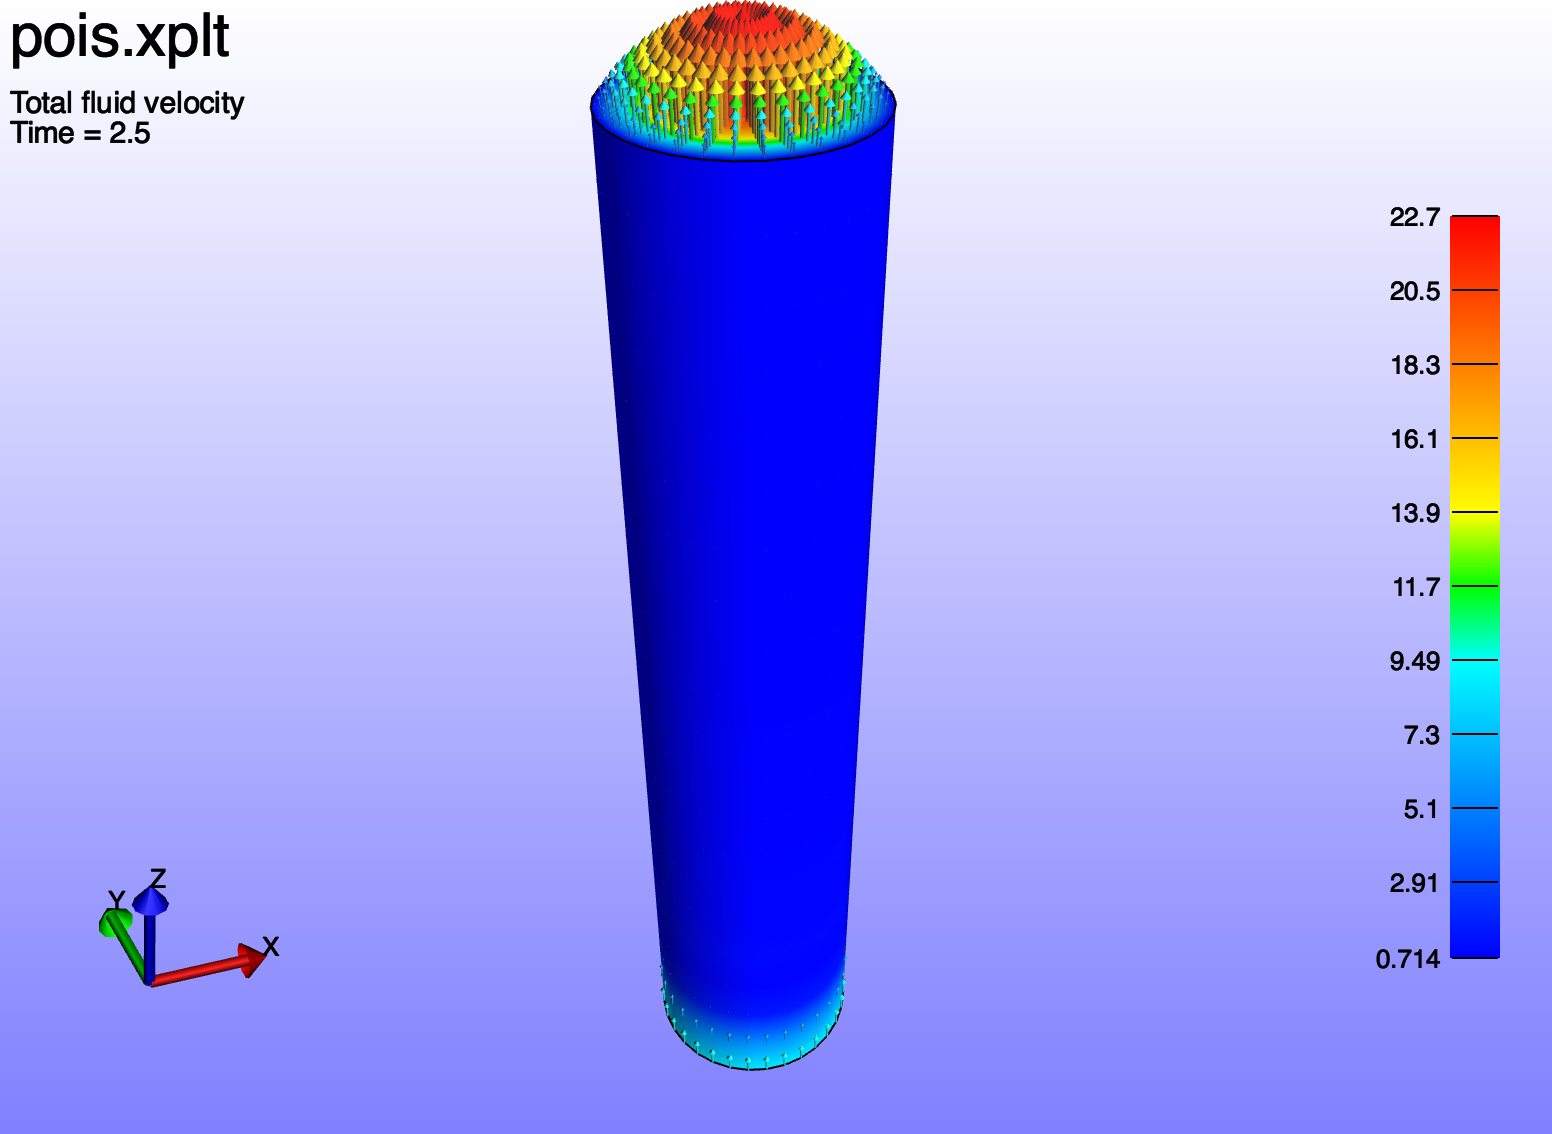
\includegraphics[width=\linewidth]{figuras_4/pois_va.png}
\caption{Campo de velocidades con vectores}
\label{fig:pois_va}
\end{subfigure}
\hfil
\begin{subfigure}[b]{0.48\textwidth}
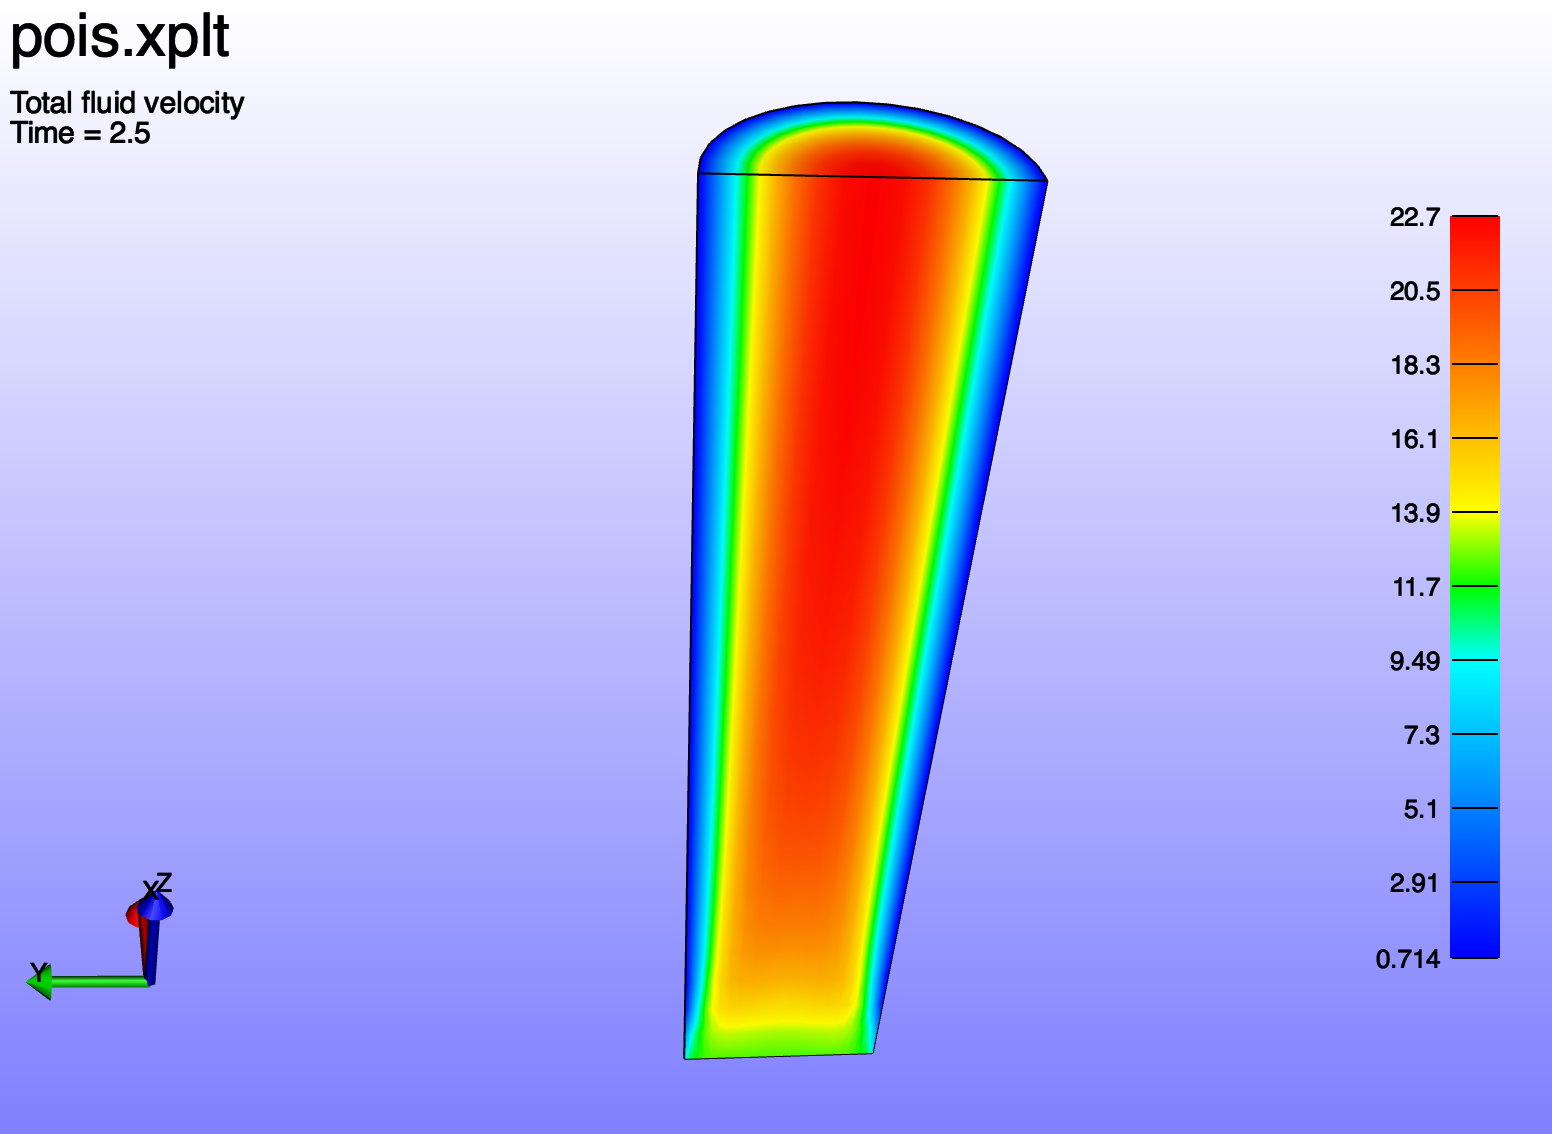
\includegraphics[width=\linewidth]{figuras_4/pois_vh1.png}
\caption{Campo de velocidades en modelo cortado}
\label{fig:pois_vh1}
\end{subfigure}
\caption{Resultados del campo de velocidades en el instante final}
\label{fig:pois_v}
\end{figure}

También se pueden obtener curvas con perfiles de distintas variables a lo largo de líneas definidas.
En la fig. \ref{fig:08-post-vprof-out-1} se muestra la selección de una línea de nodos diametral y el gráfico con los perfiles de velocidades en los distintos instantes de tiempo, que van aproximándose progresivamente a la distribución parabólica.
Análogamente se pueden obtener en la sección de entrada, en la cual la velocidad impuesta es uniforme, lo que se aprecia en la fig.~\ref{fig:08-post-vprof-in-1}.
\begin{figure}[!ht]
\centering
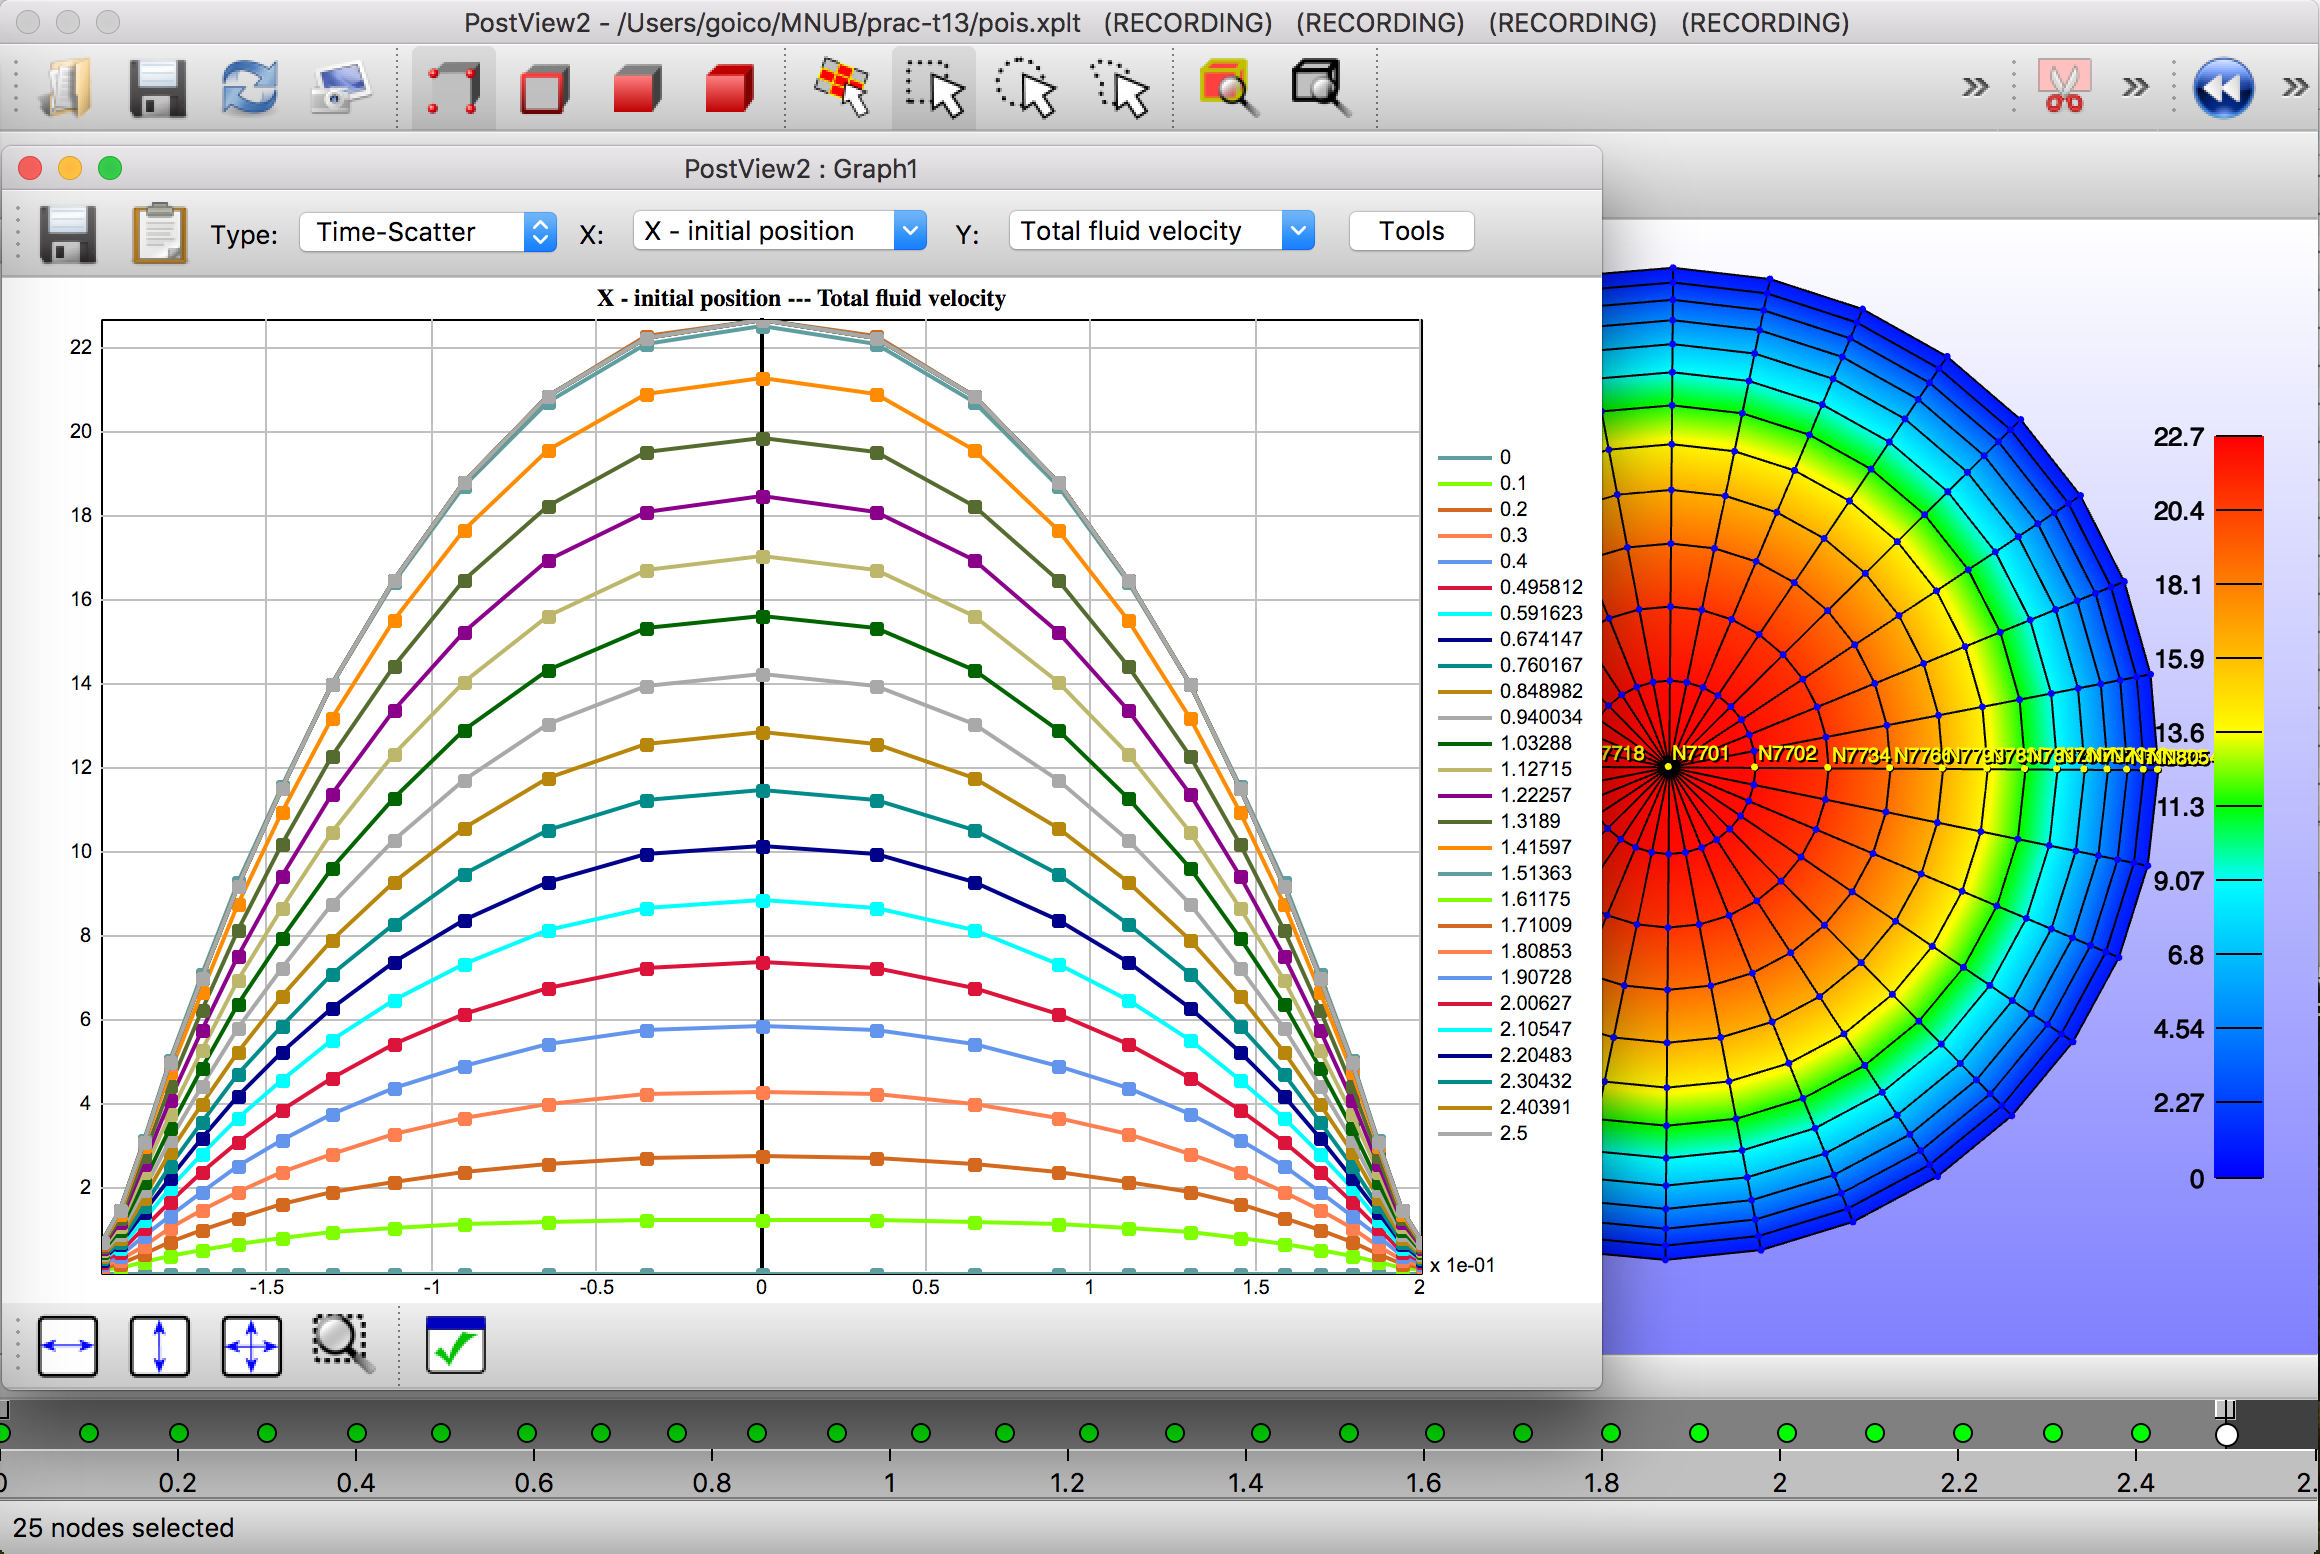
\includegraphics[width=0.5\linewidth]{figuras_4/08-post-vprof-out-1.png}
\caption{Perfil de velocidades a lo largo de una línea diametral de nodos en la sección de salida, en los distintos instantes de tiempo}
\label{fig:08-post-vprof-out-1}
\end{figure}
\begin{figure}[!ht]
\centering
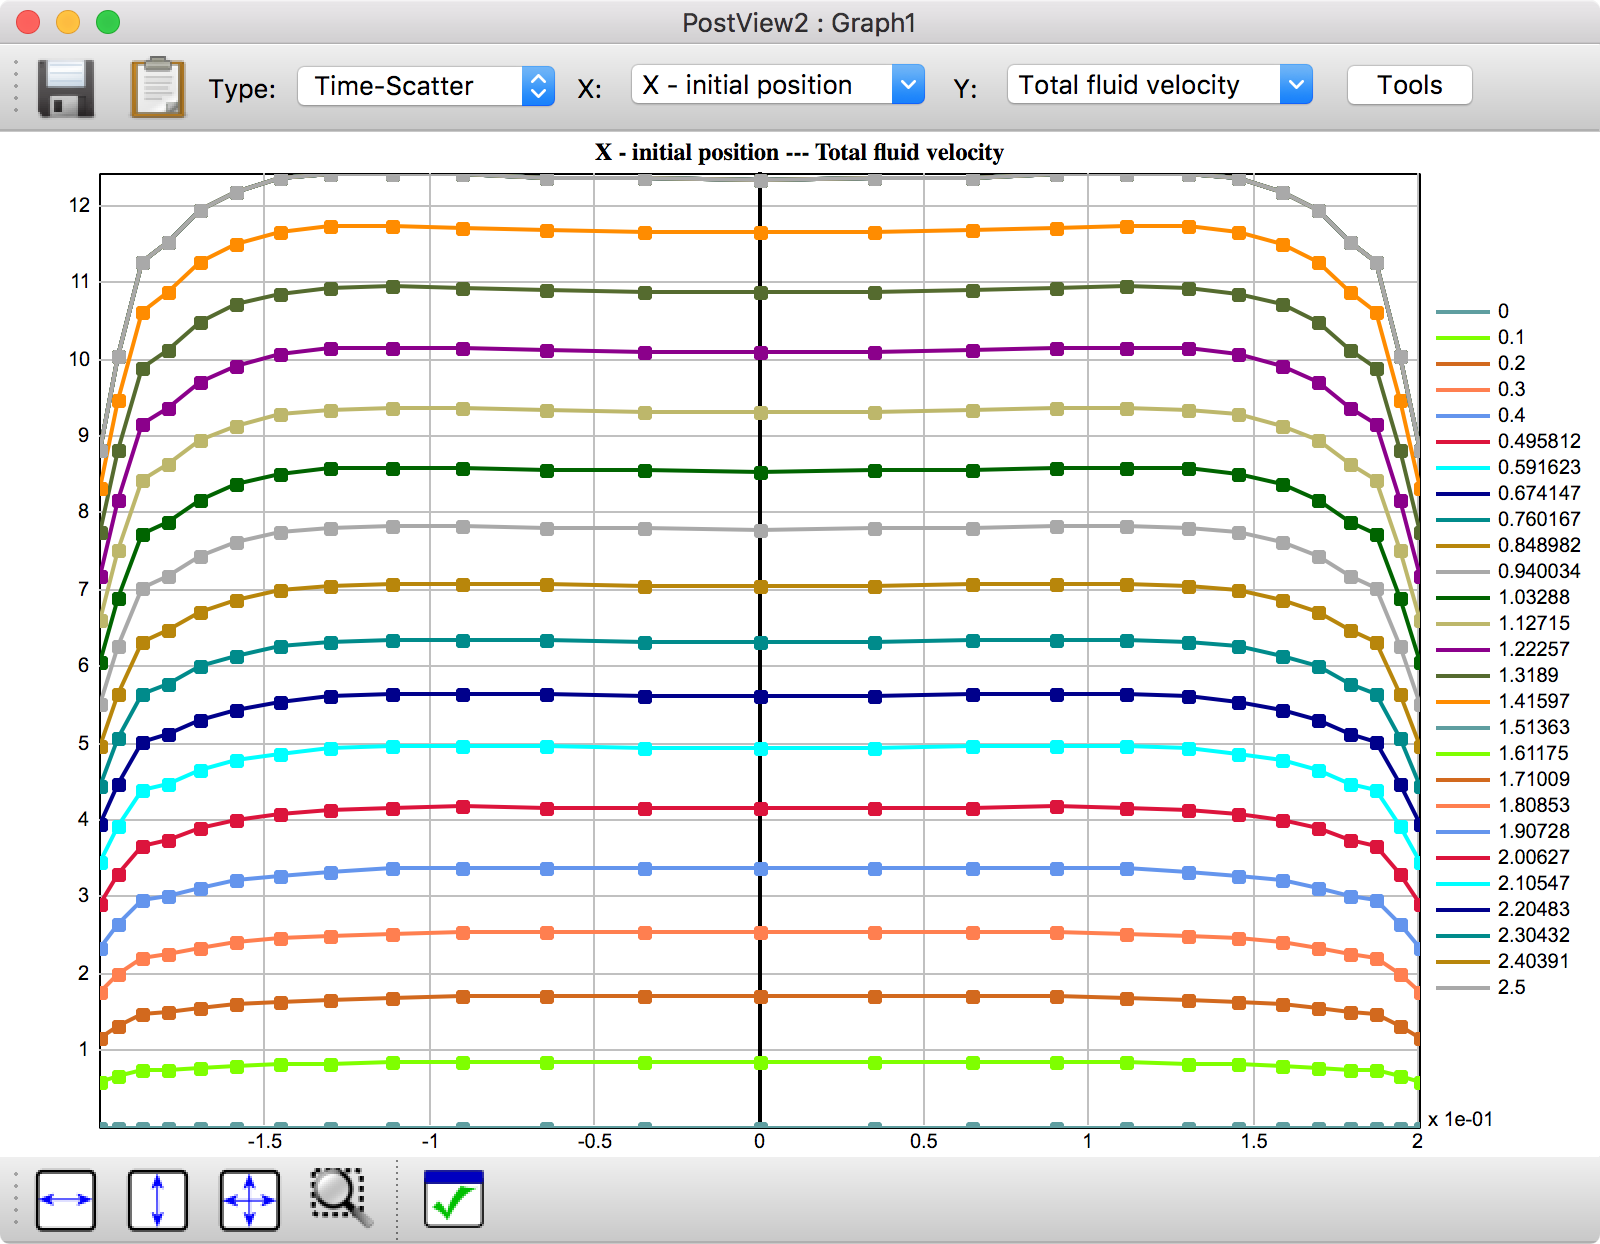
\includegraphics[width=0.5\linewidth]{figuras_4/08-post-vprof-in-1.png}
\caption{Perfil de velocidades a lo largo de una línea diametral de nodos en la sección de entrada, en los distintos instantes de tiempo}
\label{fig:08-post-vprof-in-1}
\end{figure}

Es posible limitar estas curvas para mayor claridad, seleccionando solo un instante de tiempo, mediante las opciones que se ofrecen con el botón \emph{Tools} (figs. \ref{fig:08-post-vprof-out-2}, \ref{fig:08-post-vprof-out-3}).
\begin{figure}[!ht]
\centering
\begin{subfigure}[b]{0.48\textwidth}
\centering
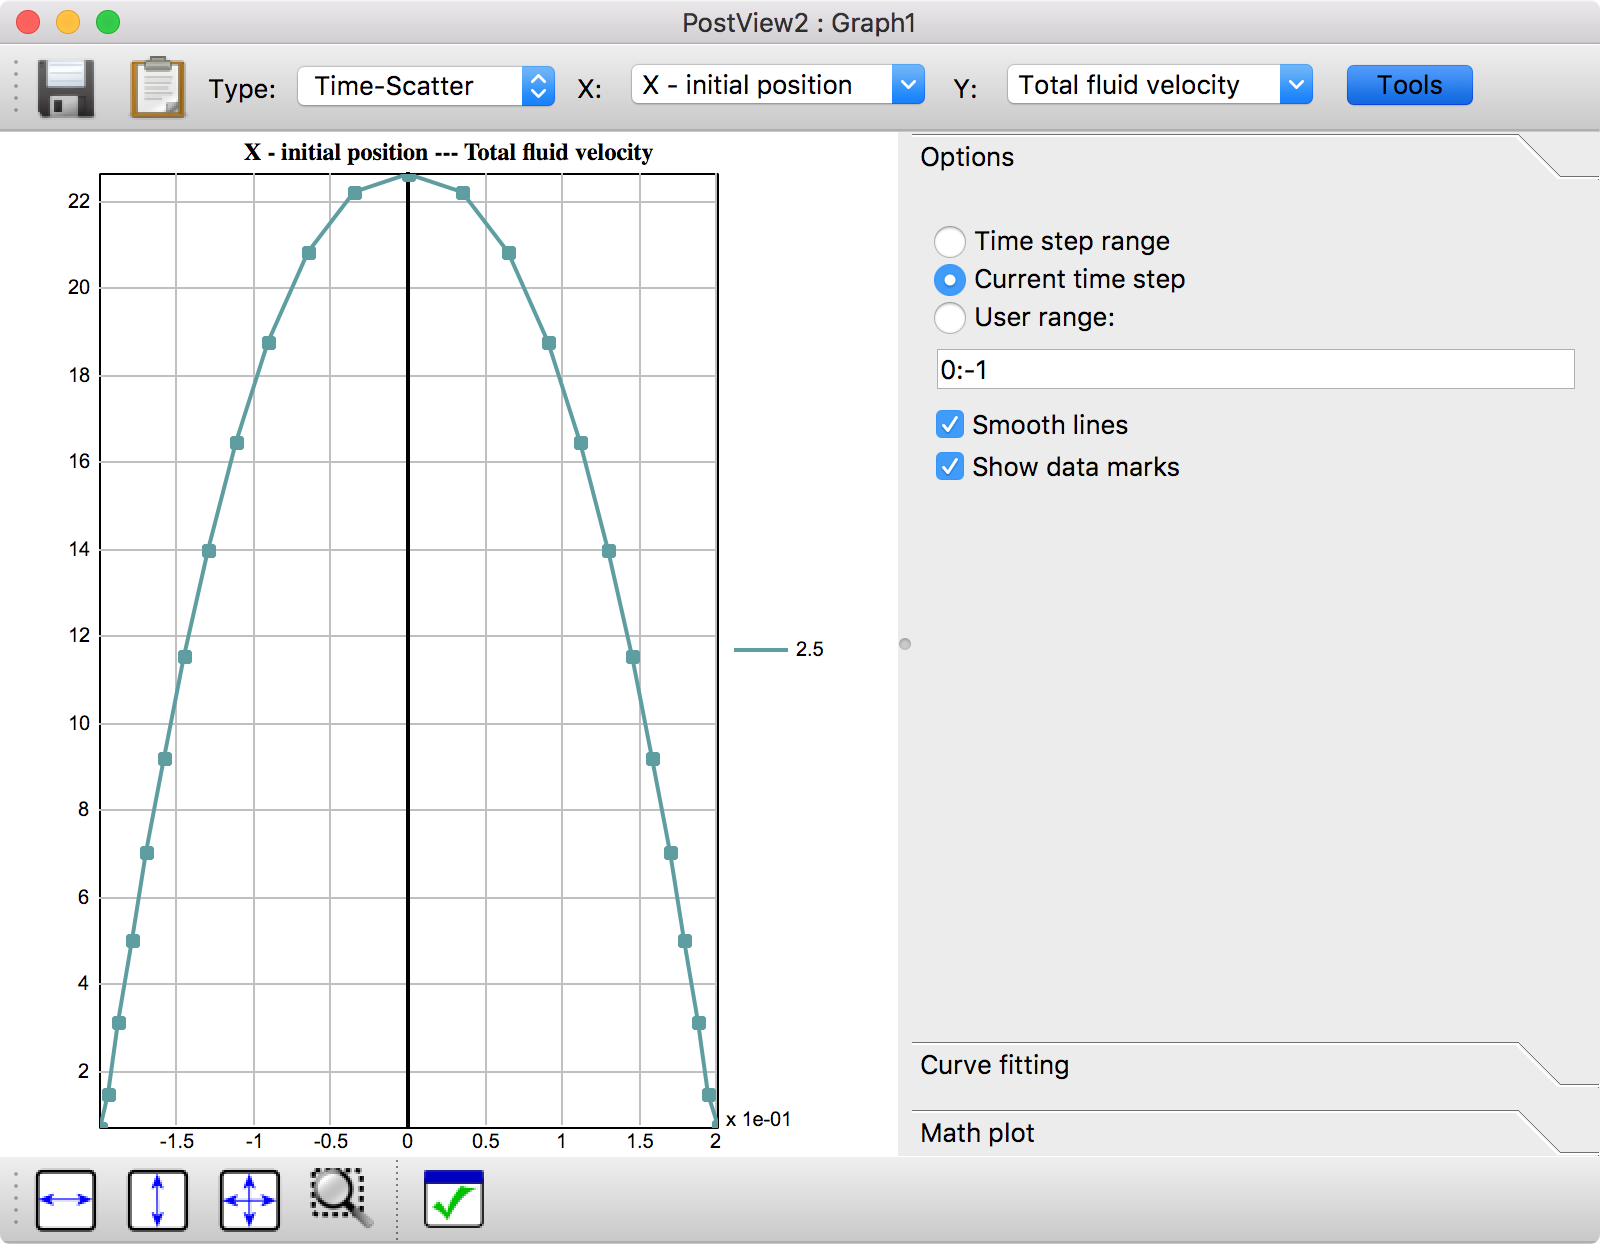
\includegraphics[width=\linewidth]{figuras_4/08-post-vprof-out-2.png}
\caption{Perfil solo en un instante}
\label{fig:08-post-vprof-out-2}
\end{subfigure}
\hfil
\begin{subfigure}[b]{0.48\textwidth}
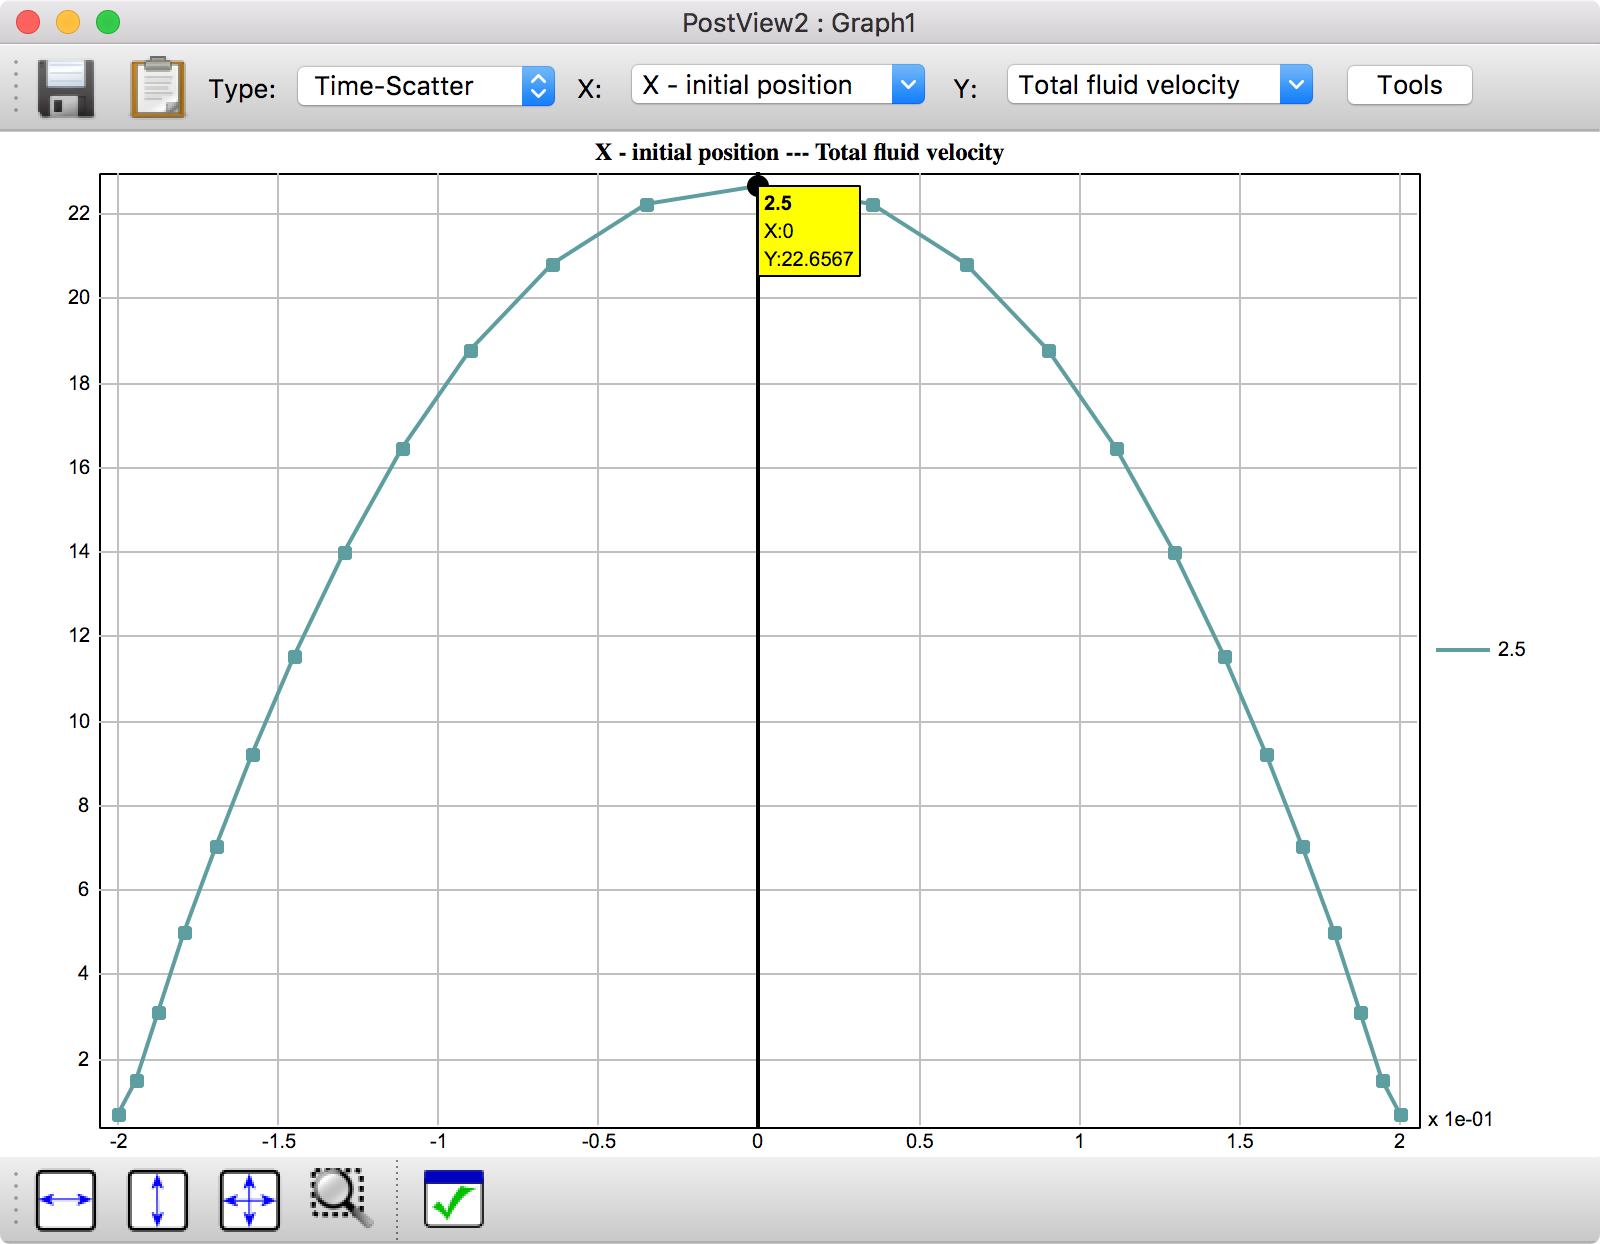
\includegraphics[width=\linewidth]{figuras_4/08-post-vprof-out-3.png}
\caption{Perfil de velocidades en instante final}
\label{fig:08-post-vprof-out-3}
\end{subfigure}
\caption{Perfil de velocidades}
\label{fig:08-post-vprof-out-2-3}
\end{figure}

En esta última ventana se puede salvar los resultados numéricos en un fichero de texto, para proceso gráfico o numérico posterior.
Eso es lo que se ha realizado en la fig.~\ref{fig:pois-vr_comp}, donde se compara con la expresión analítica del perfil parabólico teórico de Poiseuille.
En este gráfico se ha incluido también el resultado de repetir los cálculos anteriores con un modelo en el que al flujo de entrada se le daba ya un perfil parabólico mediante la activación de la casilla \emph{parabolic} (fig.~\ref{fig:pre-05-c}) y repitiendo el cálculo.
\begin{figure}[!htp]
\centering
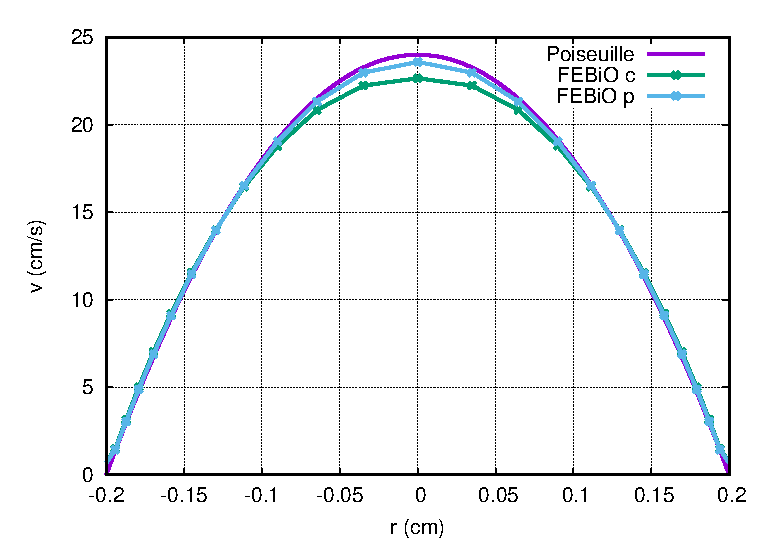
\includegraphics[width=0.6\textwidth]{figuras_4/pois-vr_comp.eps}
\caption{Resultados de velocidades en el instante final, obtenidos con FEBiO para los casos de velocidad de entrada uniforme (c) y parabólica (p) y perfil teórico de Poiseuille}
\label{fig:pois-vr_comp}
\end{figure}

\clearpage
\section{CFD en tubo curvo}
\label{sec:tubocurvo}

\subsection{Geometría, malla y material}

El primer paso es crear el modelo geométrico con el módulo \emph{Build}, en esta ocasión se trata de un toro con el radio de su directriz (\emph{Outer radius}) $R_{o}=1.273$ cm y radio de su sección circular (\emph{inner radius}) $R_{i}=0.2$ cm, como se indica en la fig.~\ref{fig:01_build-create-torus}.
\begin{figure}[!ht]
\centering
\begin{subfigure}[b]{0.28\textwidth}
\centering
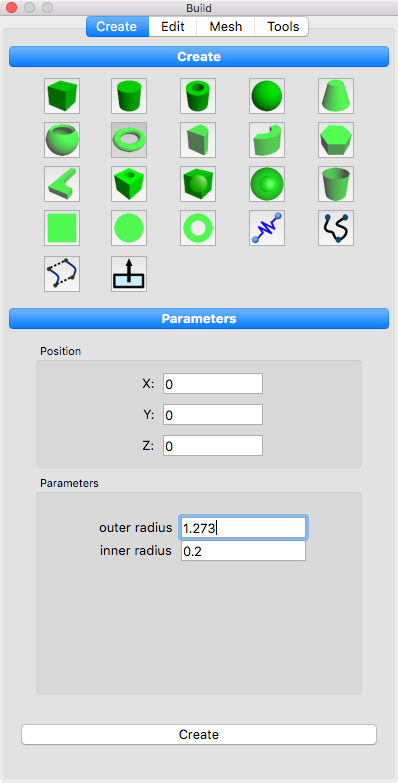
\includegraphics[width=\linewidth]{figuras_4/01_build-create.png}
\caption{Datos del toro}
\label{fig:01_build-create}
\end{subfigure}
\hfil
\begin{subfigure}[b]{0.48\textwidth}
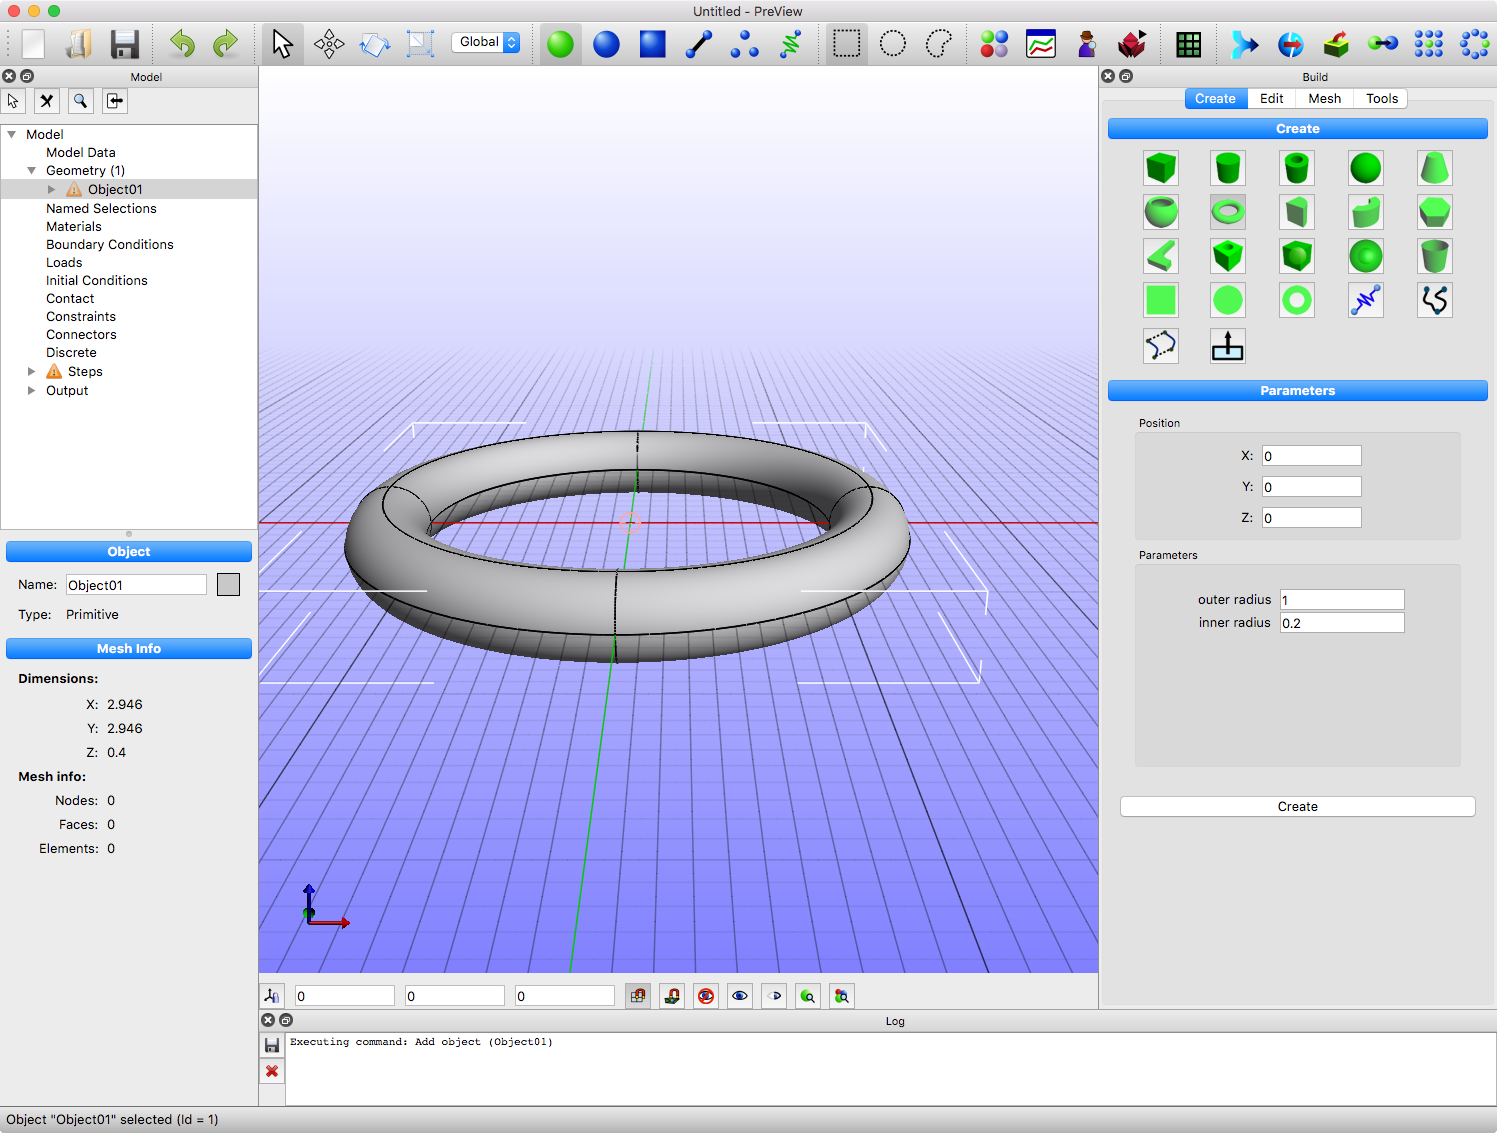
\includegraphics[width=\linewidth]{figuras_4/01_build-torus.png}
\caption{Modelo del toro}
\label{fig:01_build-torus}
\end{subfigure}
\caption{Creación de la geometría de un toro}
\label{fig:01_build-create-torus}
\end{figure}

La malla se crea con los parámetros \emph{Divisions}=4 y \emph{Segments}=16 como se indica en la fig.~\ref{fig:01_build-torusmesh}.
Ahora realizaremos varios pasos para quedarnos tan solo con $1/4$ del toro, eliminando los $3/4$ restantes.
En la pestaña \emph{Mesh} se define la malla como \emph{Editable Mesh} (fig.~\ref{fig:02_build-mesh-editable}).
\begin{figure}[!ht]
\centering
\begin{subfigure}[b]{0.30\textwidth}
\centering
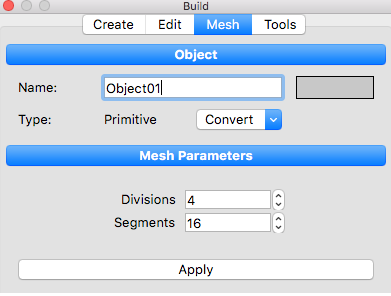
\includegraphics[width=\linewidth]{figuras_4/01_build-torusmesh.png}
\caption{Malla del toro}
\label{fig:01_build-torusmesh}
\end{subfigure}
\begin{subfigure}[b]{0.30\textwidth}
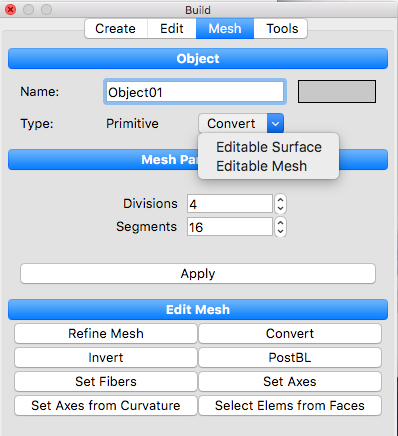
\includegraphics[width=\linewidth]{figuras_4/02_build-mesh-editable.png}
\caption{Convertir en editable}
\label{fig:02_build-mesh-editable}
\end{subfigure}
\caption{Crear malla del toro \emph{Editable}}
\label{fig:02_build-mesh-torus-editable}
\end{figure}

Para eliminar una parte del toro primero debemos activar en la barra de iconos inferior las opciones \emph{Select elements} y \emph{Select connected}, indicadas en la fig.~\ref{fig:02d_selection-bar}.
\begin{figure}[!ht]
\centering
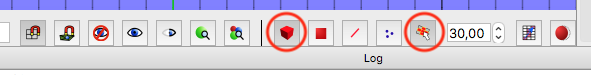
\includegraphics[width=\linewidth]{figuras_4/02d_selection-bar.png}
\caption{Activación de selección de elementos en la barra inferior para cortar el modelo}
\label{fig:02d_selection-bar}
\end{figure}
Se seleccionan ahora las partes de los 3 cuartos que se desea borrar, usando el ratón y manteniendo la tecla de mayúsculas presionada (fig.~\ref{fig:02c_build-detach-repartition}). 
Se separan (\emph{Detach}) marcando la casilla \emph{Repartition selection} (fig.~\ref{fig:03_Model-object}).
Ahora se puede visualizar el modelo que consta de dos partes (fig.~\ref{fig:03_Model-partitions}).
Se selecciona la deseada, con los 3/4 del toro, y se elimina en el módulo \emph{Model} con el botón derecho del ratón (fig.~\ref{fig:03b_Model-partition-delete}), quedando solo la cuarta parte deseada (fig.~\ref{fig:03b_Model-partition-deleted}).
En esta parte queda a la vista las secciones del toro, pudiéndose representar la malla (tecla \texttt{m}), ver fig.~\ref{fig:03d_Model-view-mesh}.
\begin{figure}[!htp]
\centering
\begin{subfigure}[b]{0.48\textwidth}
\centering
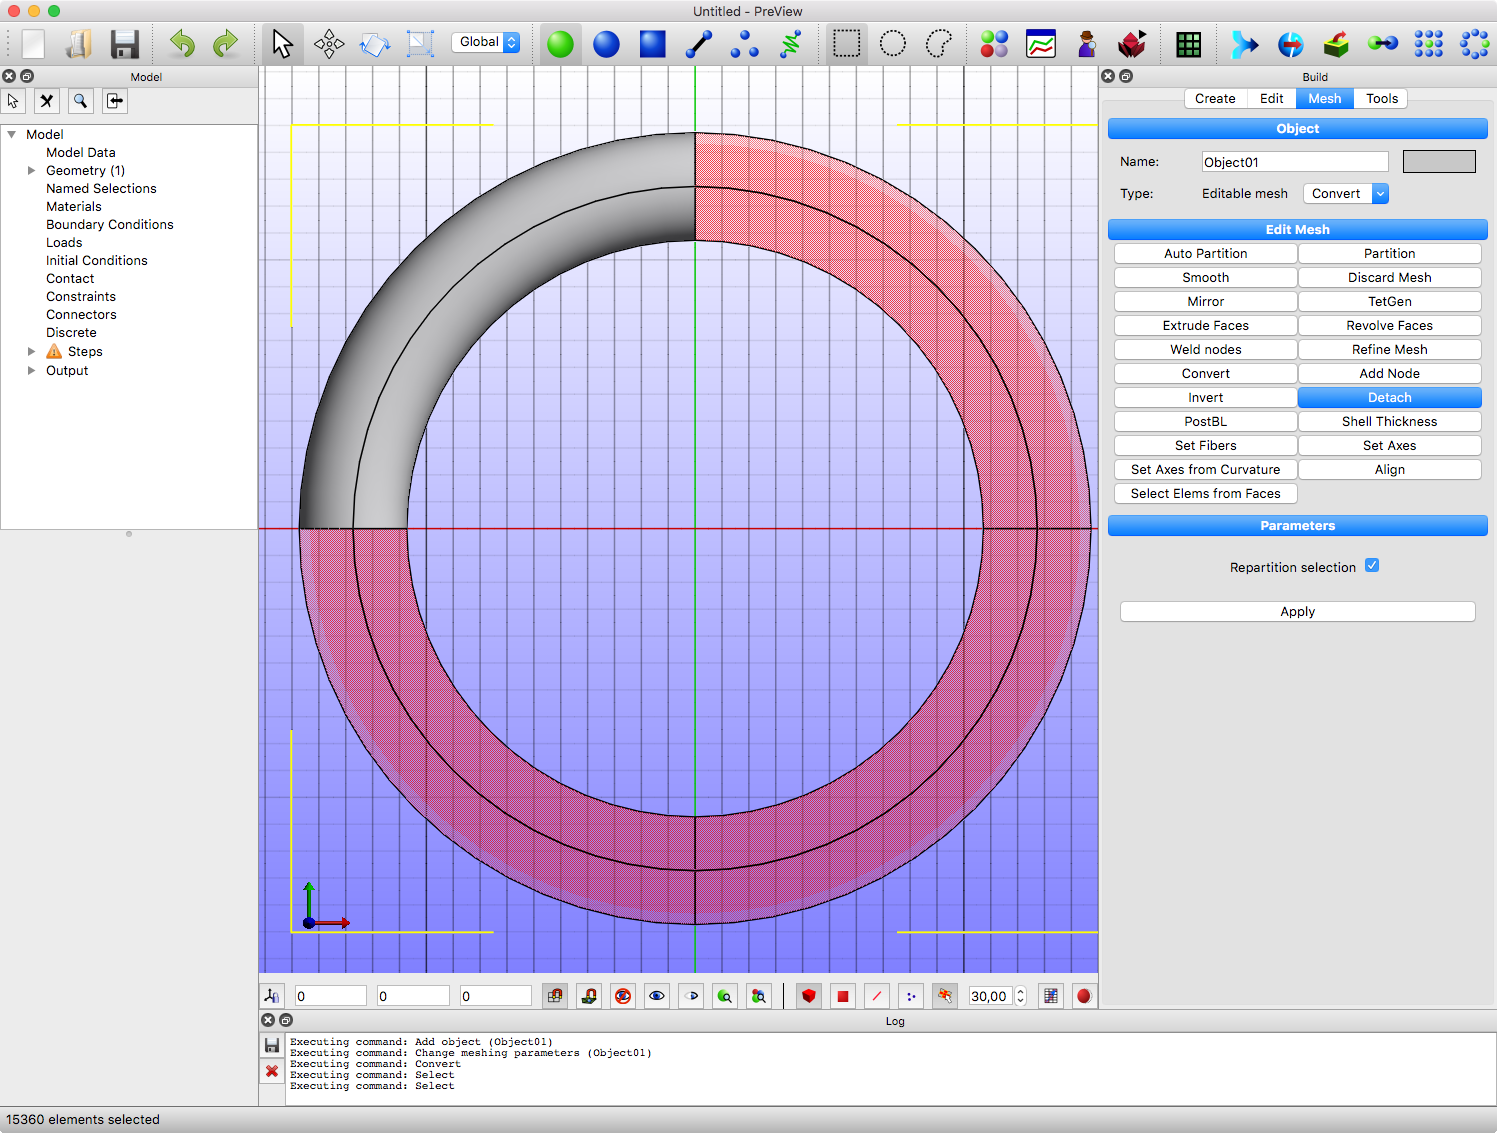
\includegraphics[width=\linewidth]{figuras_4/02c_build-detach-repartition.png}
\caption{Seleccionar 3/4 del toro}
\label{fig:02c_build-detach-repartition}
\end{subfigure}
\hfil
\begin{subfigure}[b]{0.48\textwidth}
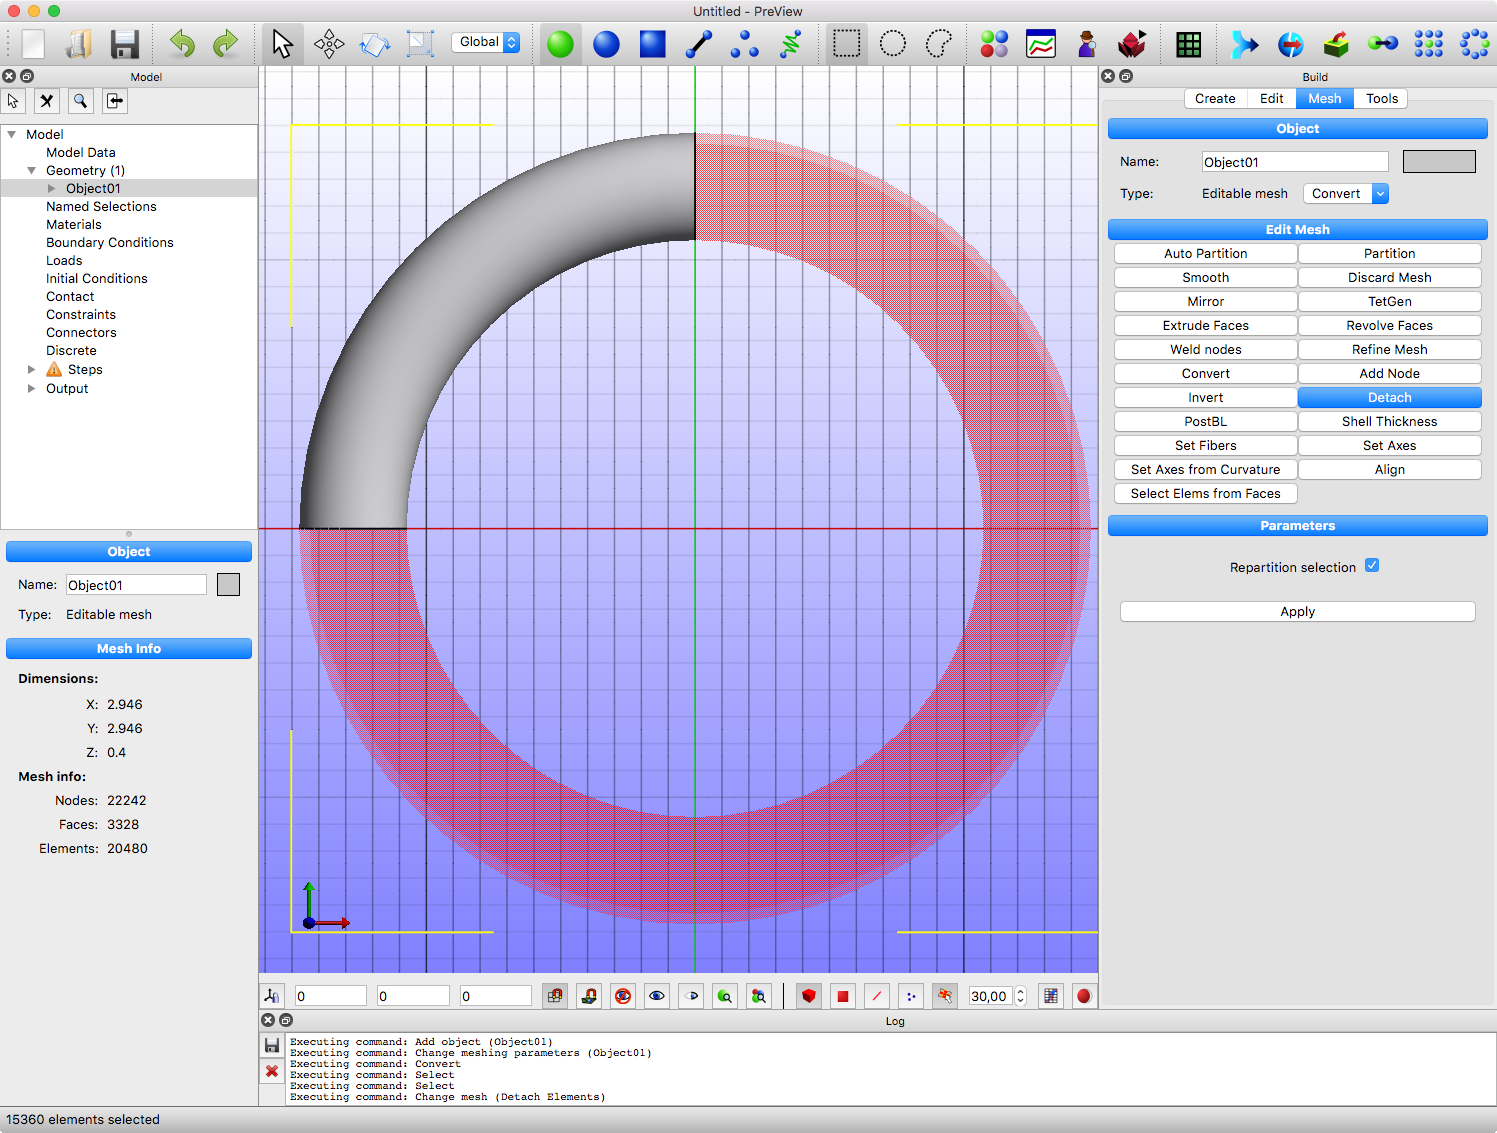
\includegraphics[width=\linewidth]{figuras_4/03_Model-object.png}
\caption{Separar 3/4 del toro}
\label{fig:03_Model-object}
\end{subfigure}
\caption{Seleccionar y separar 3/4 del toro}
\label{fig:02c-03}
\end{figure}

\begin{figure}[!htp]
\centering
\begin{subfigure}[b]{0.48\textwidth}
\centering
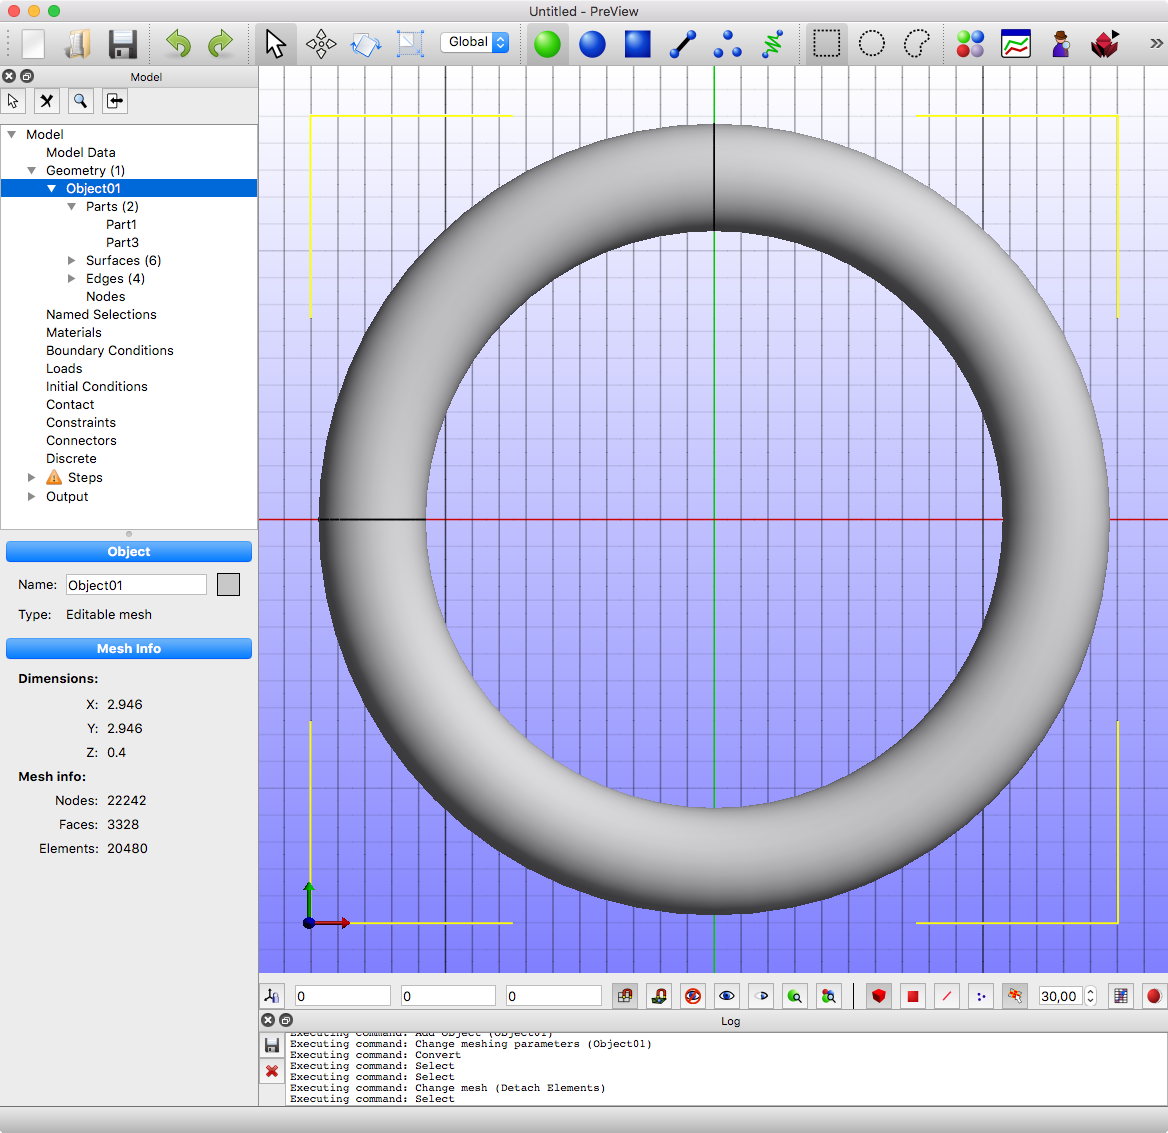
\includegraphics[width=\linewidth]{figuras_4/03_Model-partitions.png}
\caption{Particiones del modelo}
\label{fig:03_Model-partitions}
\end{subfigure}
\begin{subfigure}[b]{0.48\textwidth}
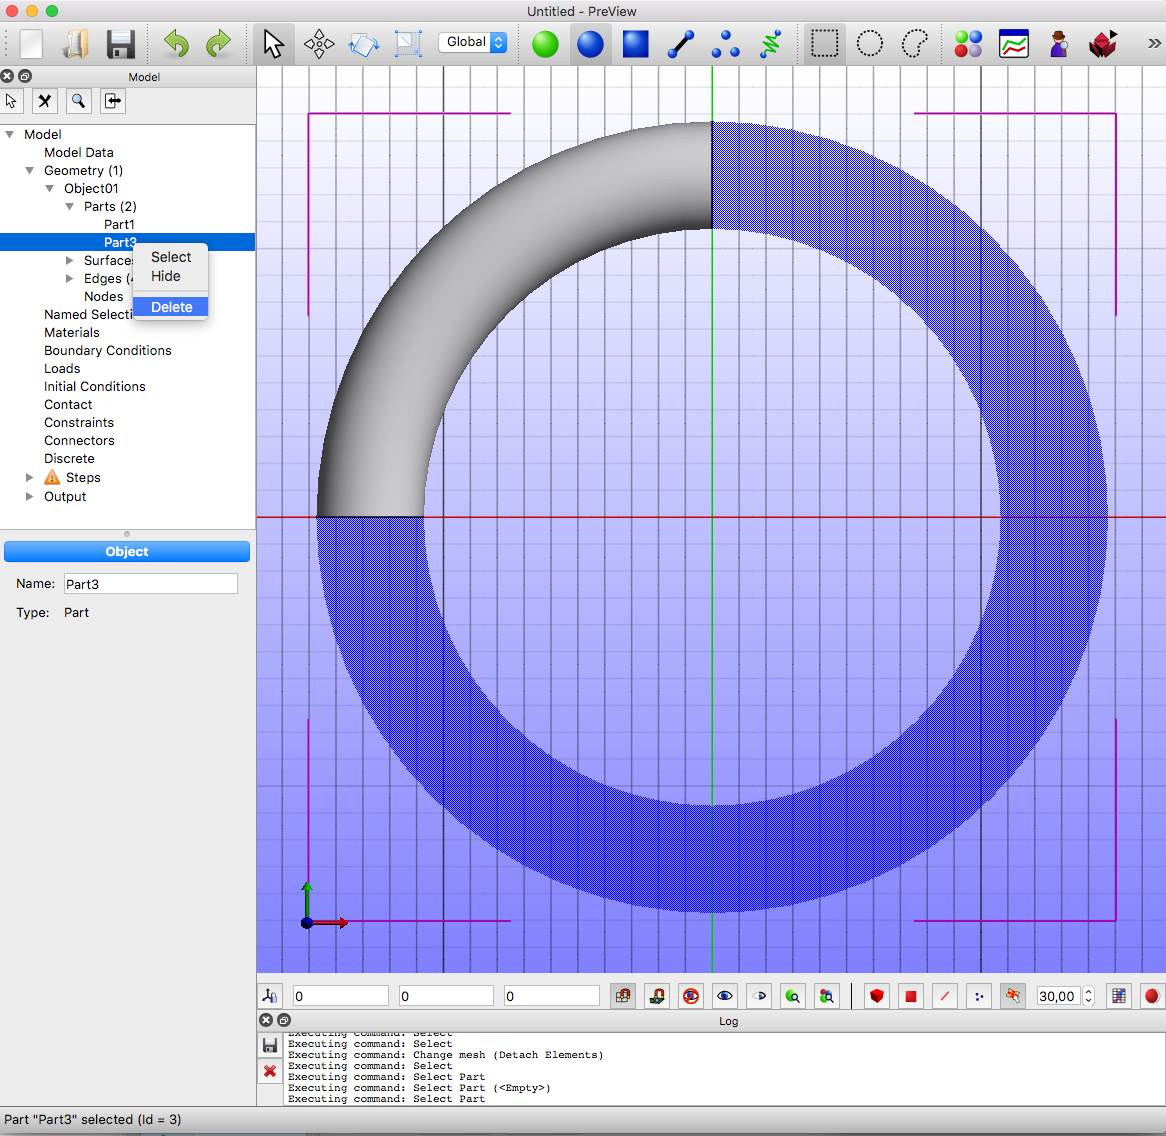
\includegraphics[width=\linewidth]{figuras_4/03b_Model-partition-delete.png}
\caption{Partición a borrar}
\label{fig:03b_Model-partition-delete}
\end{subfigure}
\caption{Eliminación de partición con 3/4 del modelo}
\label{fig:03bc}
\end{figure}

\begin{figure}[!htp]
\centering
\begin{subfigure}[b]{0.48\textwidth}
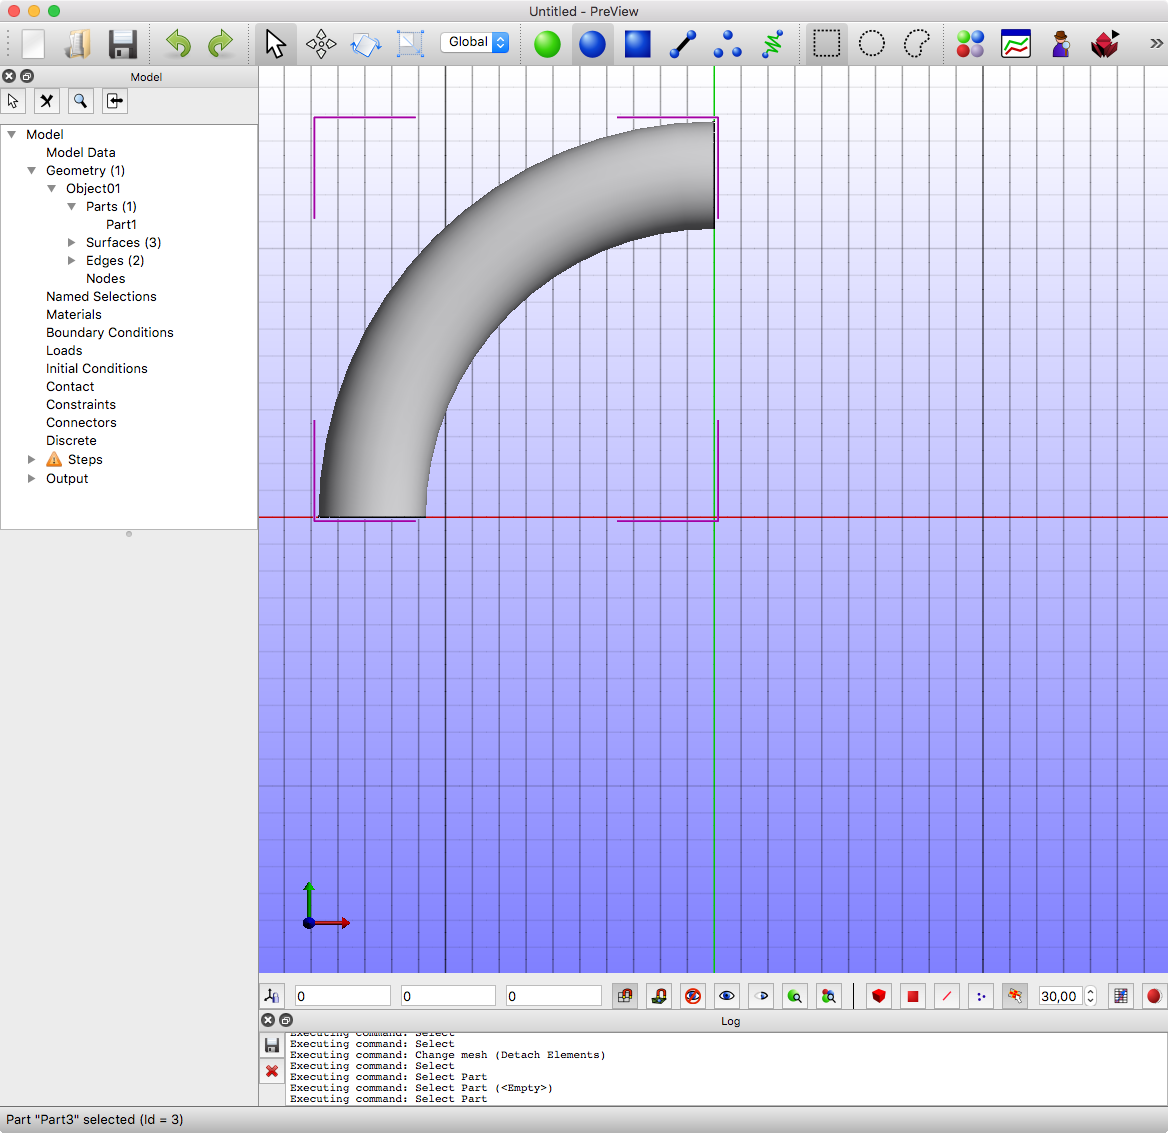
\includegraphics[width=\linewidth]{figuras_4/03b_Model-partition-deleted.png}
\caption{Partición borrada}
\label{fig:03b_Model-partition-deleted}
\end{subfigure}
\begin{subfigure}[b]{0.48\textwidth}
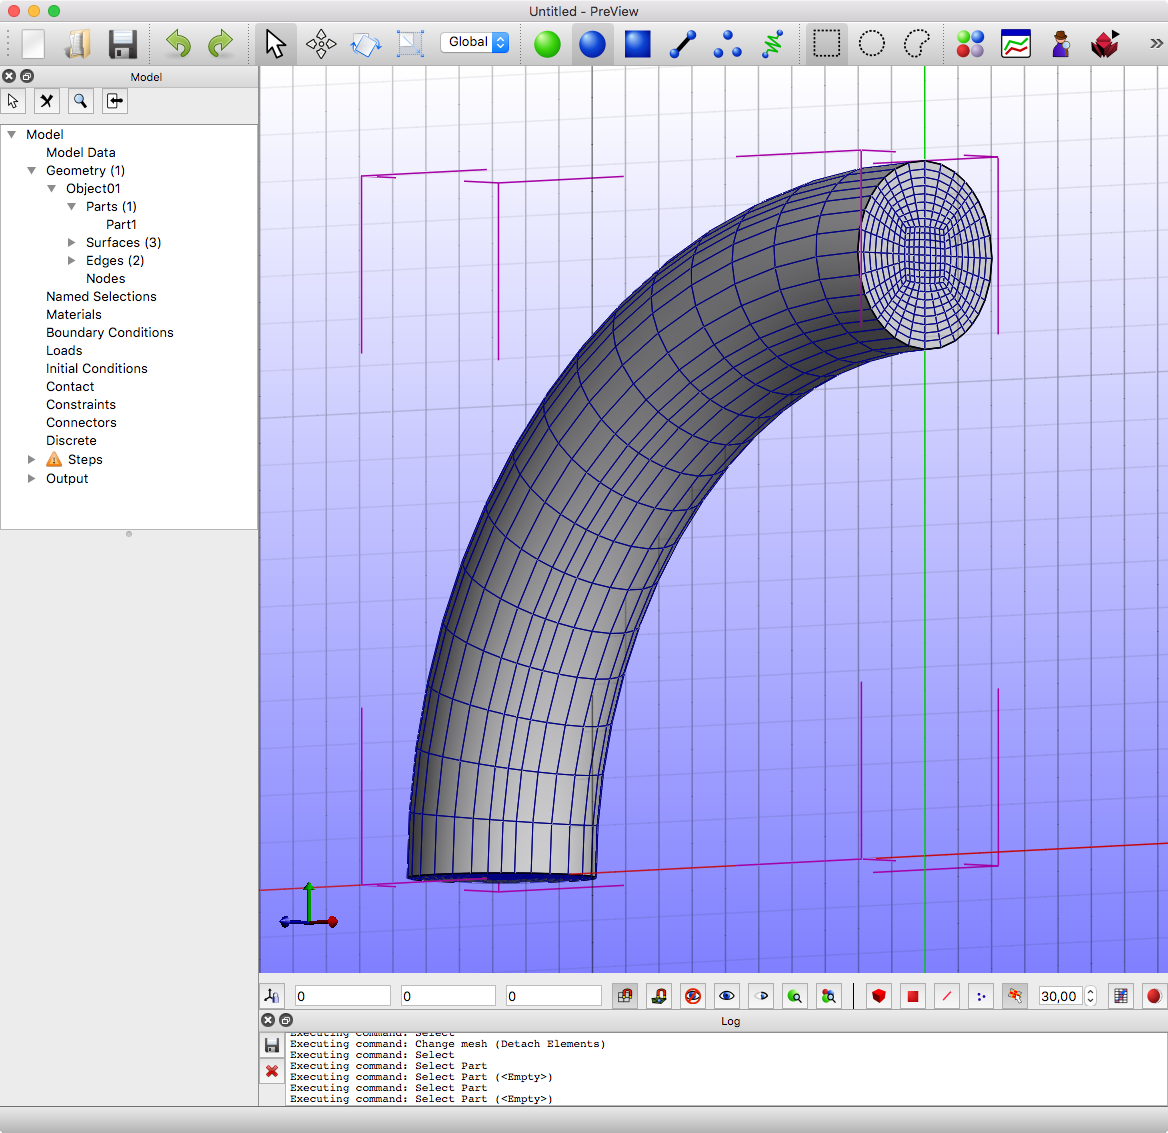
\includegraphics[width=\linewidth]{figuras_4/03d_Model-view-mesh.png}
\caption{Malla del cuarto de toro resultante}
\label{fig:03d_Model-view-mesh}
\end{subfigure}
\caption{Modelo del tubo curvo resultante}
\label{fig:03bd}
\end{figure}

El material se define con los mismos parámetros e idéntico procedimiento al empleado en la sección~\ref{sec:tuborecto} para el tubo recto, fig.~\ref{fig:04dc_material}.
\begin{figure}[!ht]
\centering
\begin{subfigure}[b]{0.25\textwidth}
\centering
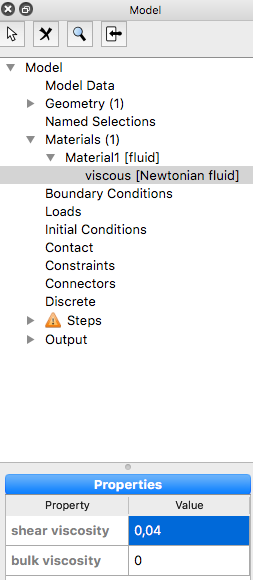
\includegraphics[width=\linewidth]{figuras_4/04d_material.png}
\caption{Datos de viscosidad}
\label{fig:04d_material}
\end{subfigure}
\hfil
\begin{subfigure}[b]{0.58\textwidth}
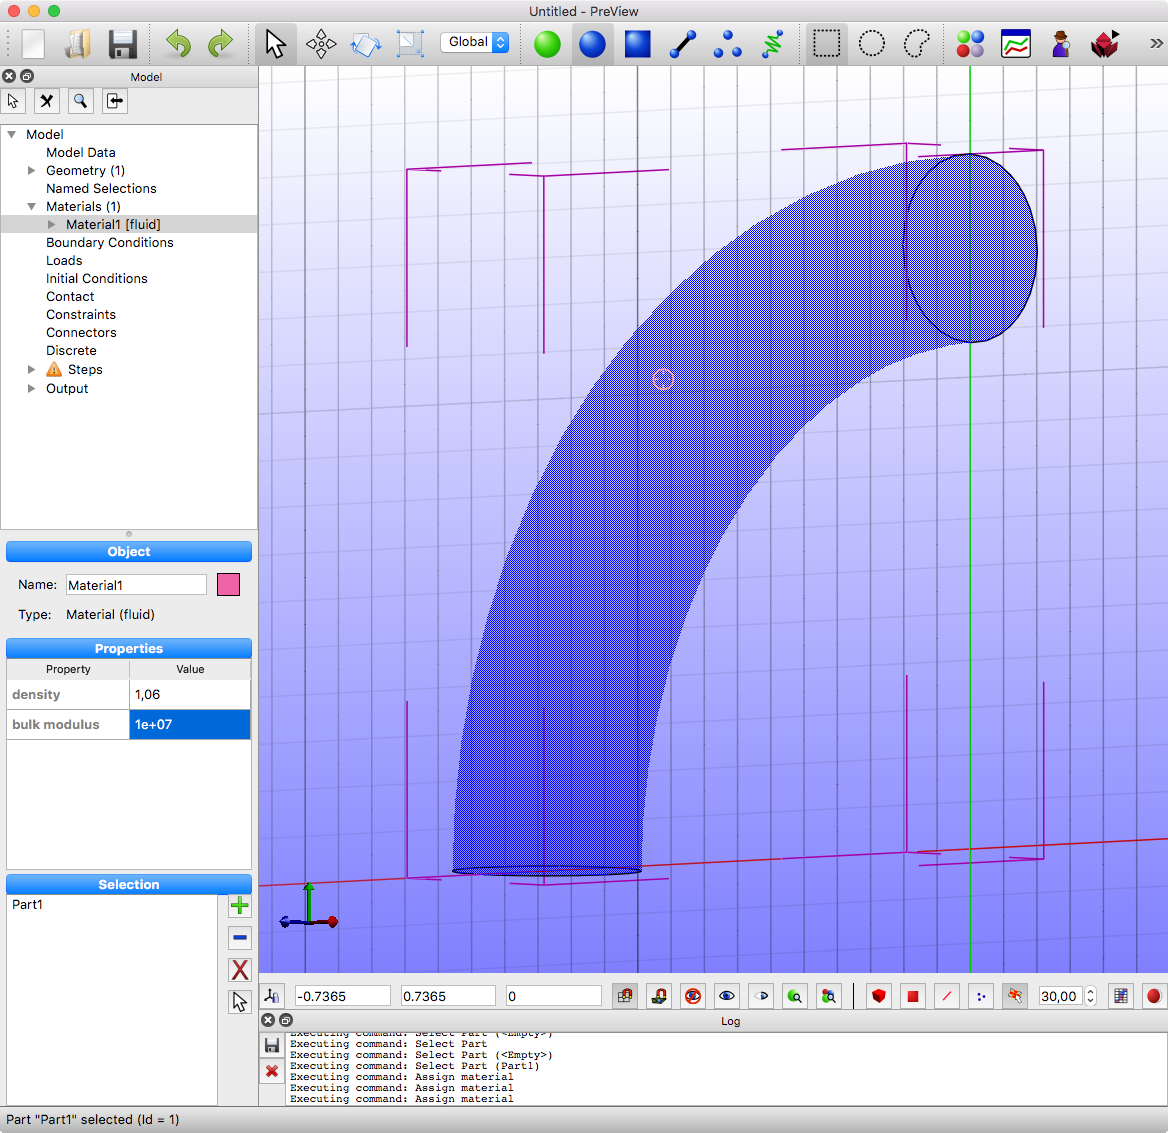
\includegraphics[width=\linewidth]{figuras_4/04c_material.png}
\caption{Asignación de material}
\label{fig:04c_material}
\end{subfigure}
\caption{Asignación de material fluido y propiedades}
\label{fig:04dc_material}
\end{figure}

\clearpage
\subsection{Condiciones de contorno y cargas}

El proceso para definir las condiciones de contorno es también el mismo que el empleado para el tubo recto en la sección~\ref{sec:tuborecto}.
Se indican las condiciones de contorno y la velocidad normal aplicada en las figs.~\ref{fig:05_bc_zfv1b}, \ref{fig:06_bc_zfd1b}, \ref{fig:06_bc_zfd2} y \ref{fig:07_load-fnv-2}.
Al flujo de entrada (velocidad impuesta) se le aplica una curva que alcanza el 100\% del valor en el tiempo $t=1.5$ (fig.~\ref{fig:07_load-fnv-3curve}).
\begin{figure}[!ht]
\centering
\begin{subfigure}[b]{0.48\textwidth}
\centering
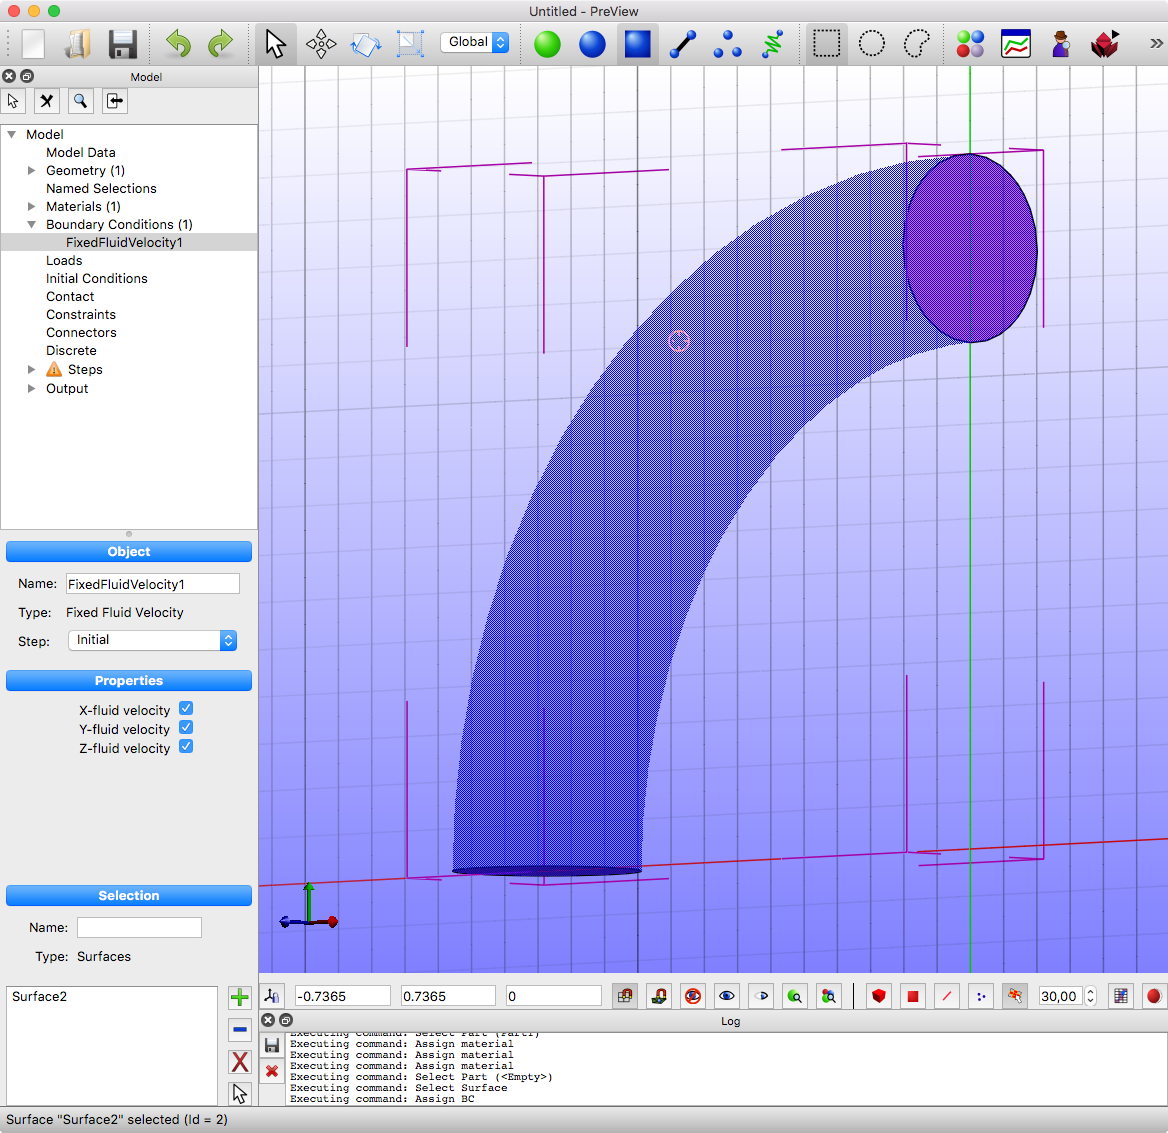
\includegraphics[width=\linewidth]{figuras_4/05_bc_zfv1b.png}
\caption{Velocidad nula en superficie externa}
\label{fig:05_bc_zfv1b}
\end{subfigure}
\hfil
\begin{subfigure}[b]{0.48\textwidth}
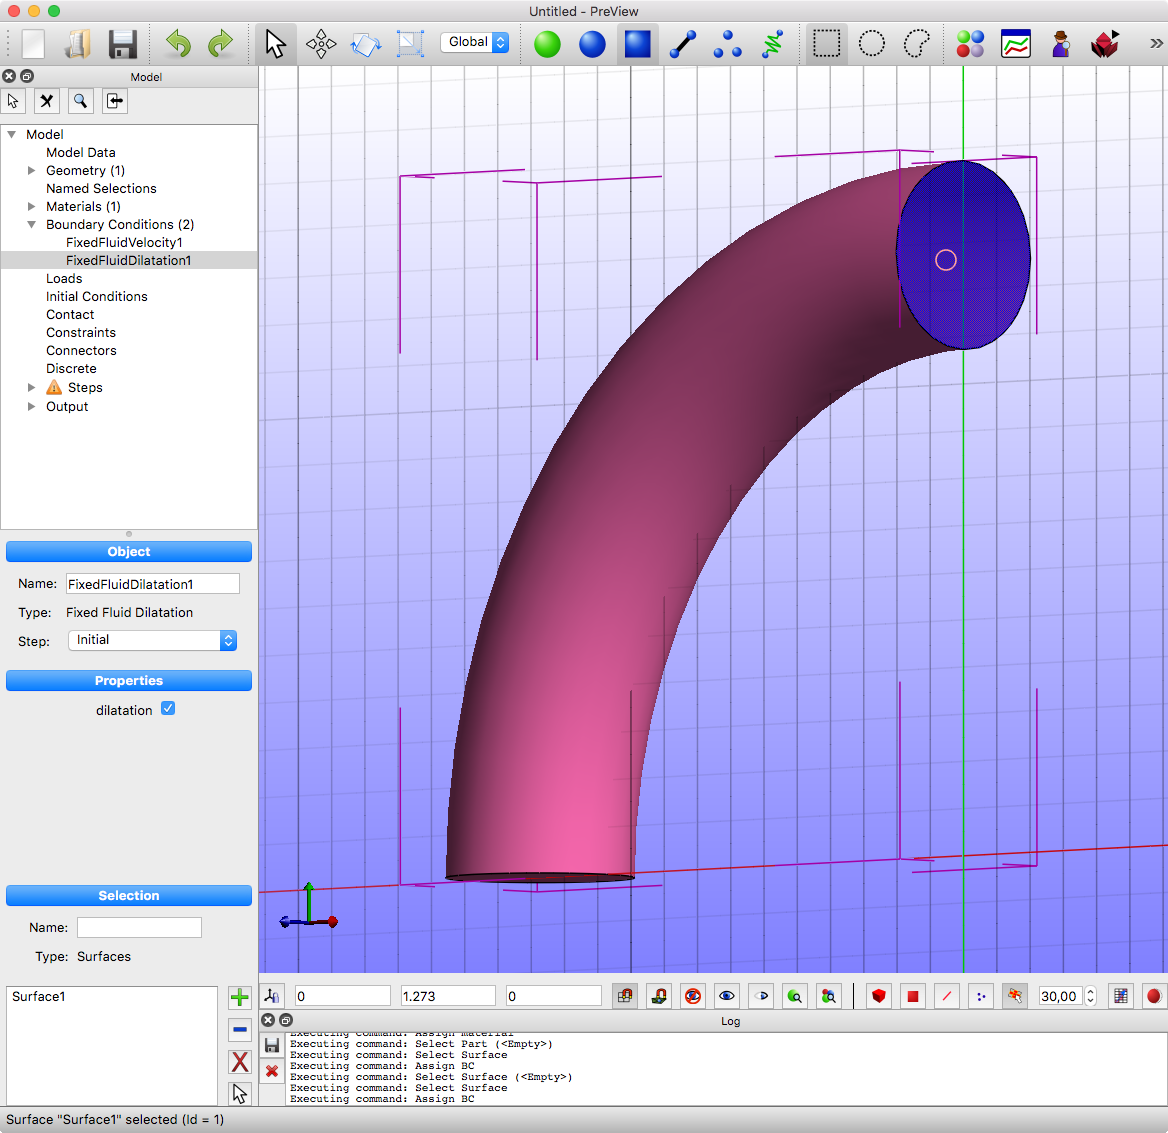
\includegraphics[width=\linewidth]{figuras_4/06_bc_zfd1b.png}
\caption{Presión nula en sección de salida}
\label{fig:06_bc_zfd1b}
\end{subfigure}
\caption{Condiciones de contorno (1)}
\label{fig:qtor-cc1}
\end{figure}

\begin{figure}[!ht]
\centering
\begin{subfigure}[b]{0.48\textwidth}
\centering
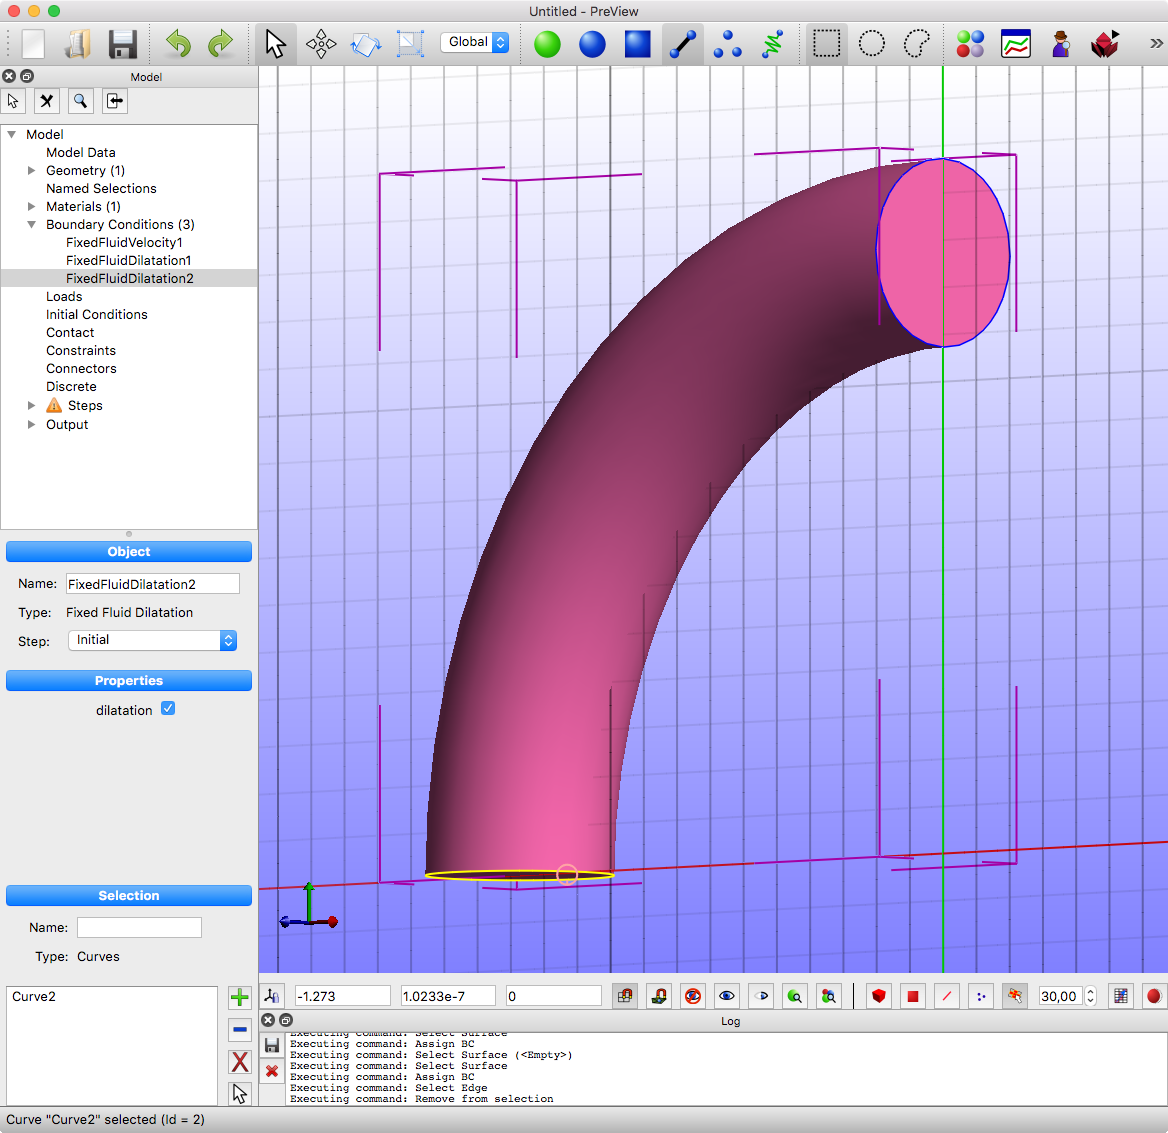
\includegraphics[width=\linewidth]{figuras_4/06_bc_zfd2.png}
\caption{Presión nula en borde de entrada}
\label{fig:06_bc_zfd2}
\end{subfigure}
\hfil
\begin{subfigure}[b]{0.48\textwidth}
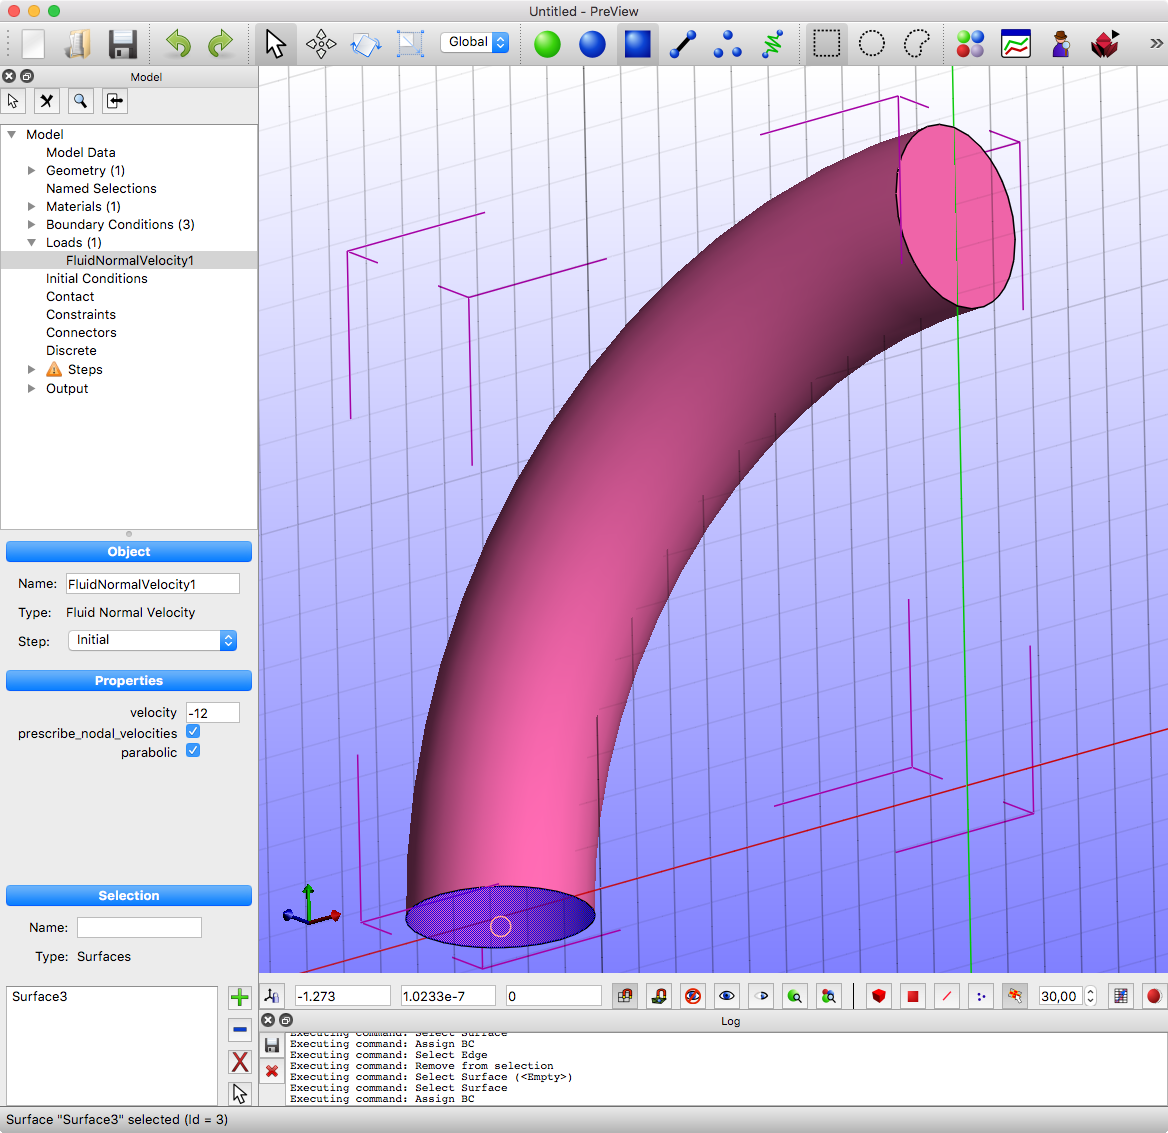
\includegraphics[width=\linewidth]{figuras_4/07_load-fnv-2.png}
\caption{Velocidad normal en sección de entrada}
\label{fig:07_load-fnv-2}
\end{subfigure}
\caption{Condiciones de contorno (2)}
\label{fig:fig:qtor-cc1}
\end{figure}

\begin{figure}[!ht]
\centering
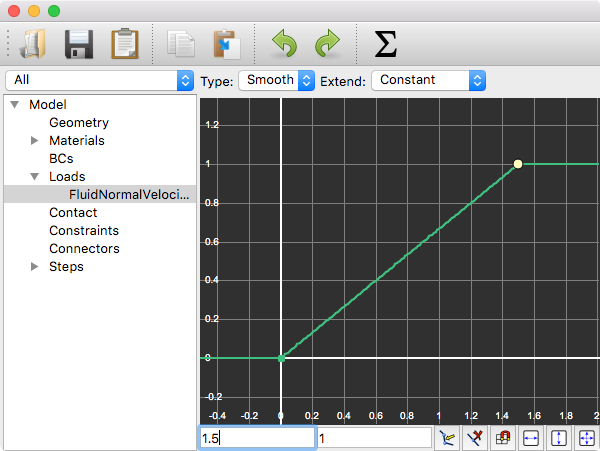
\includegraphics[width=0.40\linewidth]{figuras_4/07_load-fnv-3curve.png}
\caption{Curva de aplicación del flujo de entrada}
\label{fig:07_load-fnv-3curve}
\end{figure}

\subsection{Caso de cálculo}

Por último, se añade un Step de cálculo, con los mismos parámetros que se emplearon en la sección~\ref{sec:tuborecto} (fig.~\ref{fig:08_step-add-4}).
Una vez completado el modelo, se salva el fichero \texttt{.prv} y se exporta el \texttt{.feb} para realizar el cálculo con FEBiO.
\begin{figure}[!ht]
\centering
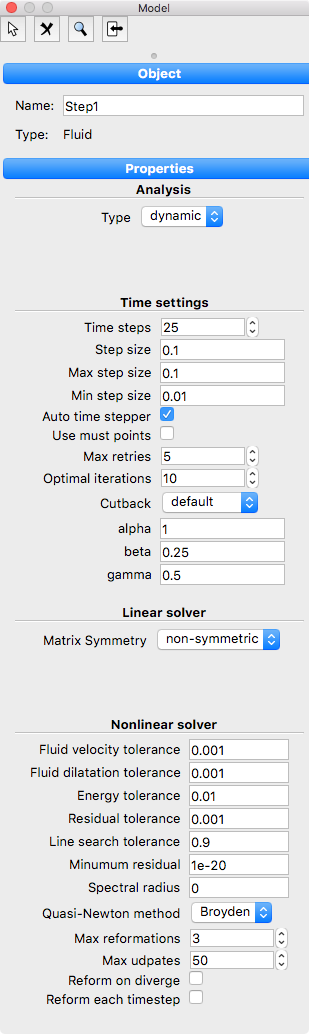
\includegraphics[width=0.25\linewidth]{figuras_4/08_step-add-4.png}
\caption{Parámetros del \emph{Step} de cálculo}
\label{fig:08_step-add-4}
\end{figure}

\subsection{Resultados}

Una vez ejecutado con éxito el cálculo, mediante el programa \emph{Postview} se pueden visualizar los distintos campos, como por ejemplo las velocidades del fluido, para lo que hemos realizado el corte por un plano perpendicular a $z$ (fig.~\ref{fig:qtor-v25aa}).
\begin{figure}[!ht]
\centering
\begin{subfigure}[b]{0.48\textwidth}
\centering
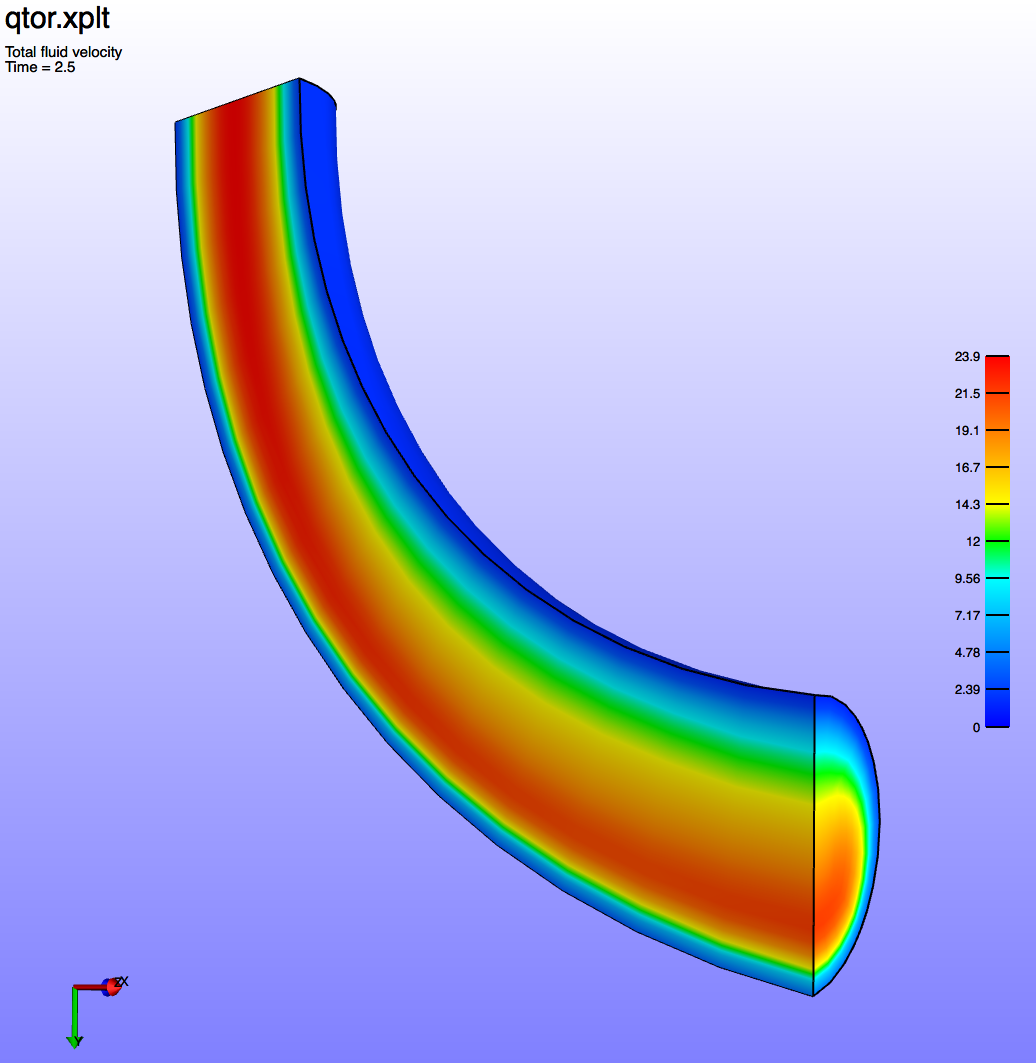
\includegraphics[width=\linewidth]{figuras_4/qtor-v25.png}
\caption{Mapa de velocidades del fluido}
\label{fig:qtor-v25}
\end{subfigure}
\hfil
\begin{subfigure}[b]{0.48\textwidth}
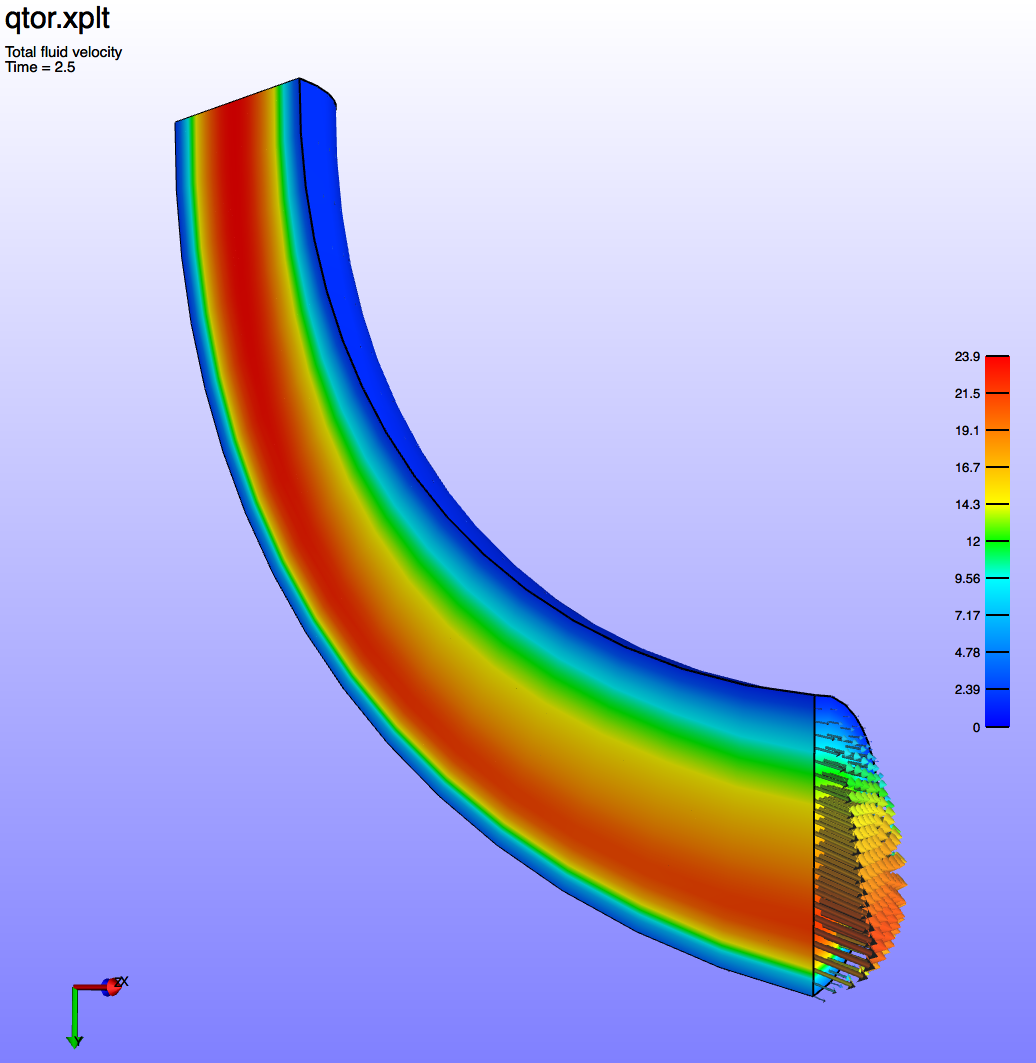
\includegraphics[width=\linewidth]{figuras_4/qtor-v25a.png}
\caption{Mapa de velocidades con vectores}
\label{fig:qtor-v25a}
\end{subfigure}
\caption{Campo de velocidades del fluido}
\label{fig:qtor-v25aa}
\end{figure}

Se seleccionan los perfiles de velocidades, tanto en la sección de salida (fig.~\ref{fig:13_post-profile-out-123}) como en la entrada (fig.~\ref{fig:14_post-profile-in}).
También se pueden guardar los datos en ficheros de texto y dibujar los gráficos comparativos (fig.~\ref{fig:qtor-vr_comp}).
En estos gráficos se observa claramente la distorsión que produce la curvatura del tubo respecto al flujo de Poiseuille.
\begin{figure}[!ht]
\centering
\begin{subfigure}[b]{0.48\textwidth}
\centering
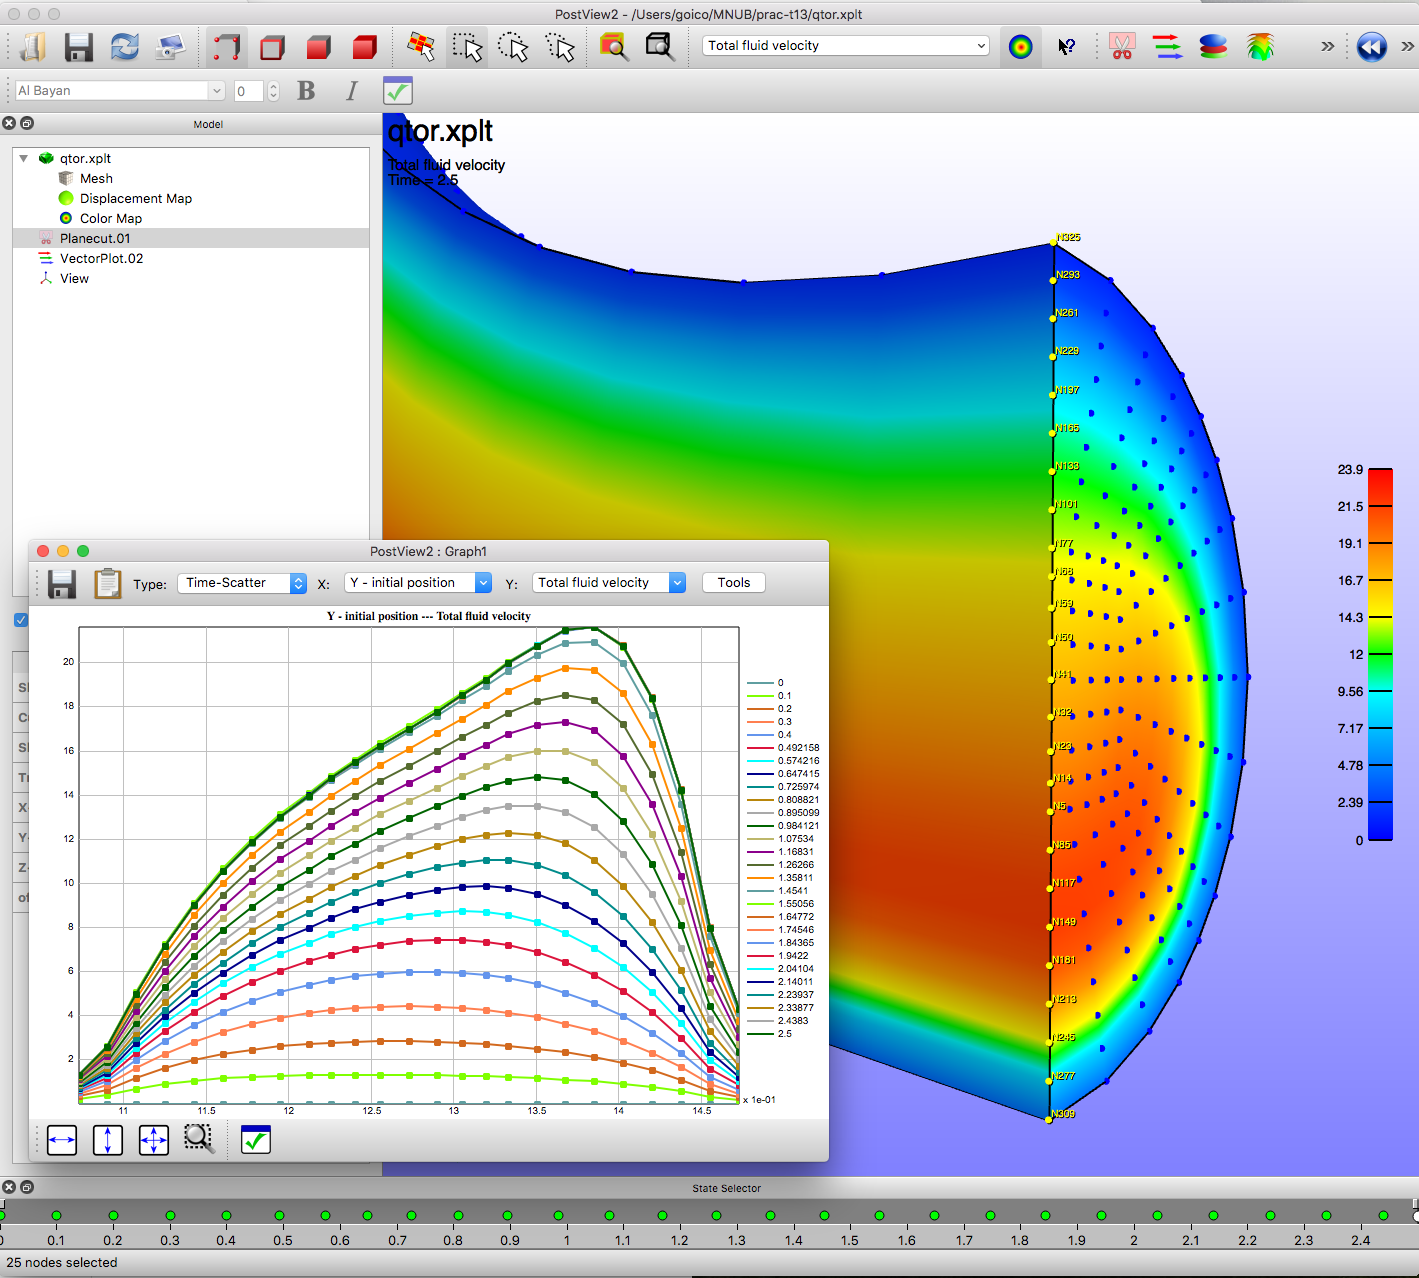
\includegraphics[width=\linewidth]{figuras_4/13_post-profile-out-1.png}
\caption{}
\label{fig:13_post-profile-out-1}
\end{subfigure}
\hfil
\begin{subfigure}[b]{0.25\textwidth}
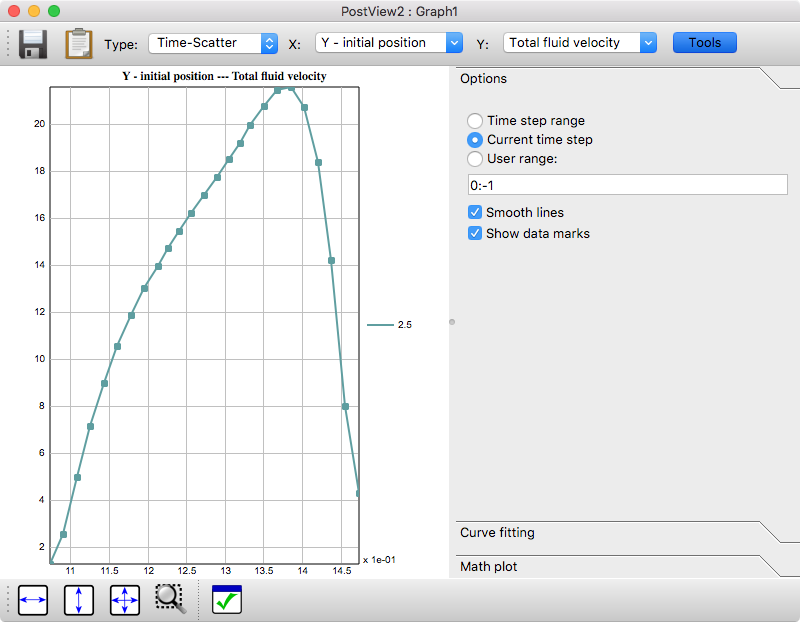
\includegraphics[width=\linewidth]{figuras_4/13_post-profile-out-2.png}
\caption{}
\label{fig:13_post-profile-out-2}
\end{subfigure}
\begin{subfigure}[b]{0.25\textwidth}
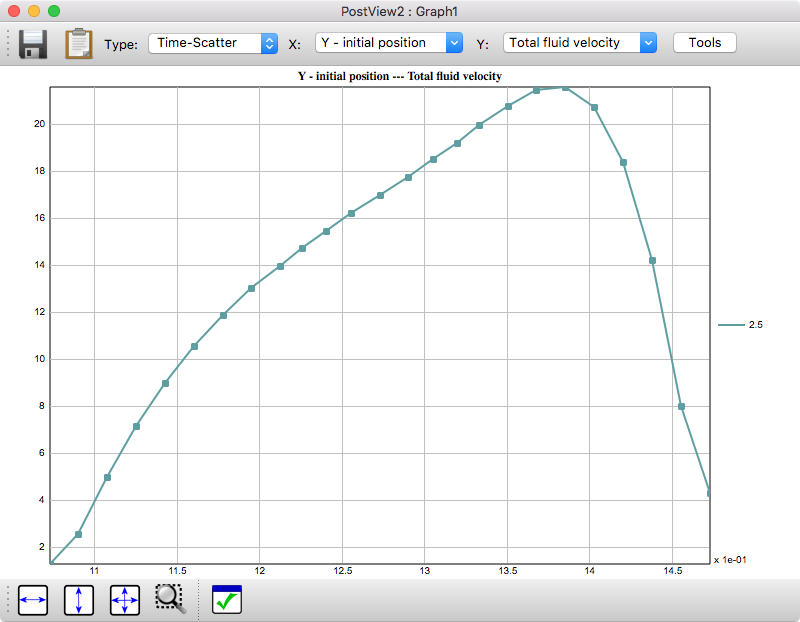
\includegraphics[width=\linewidth]{figuras_4/13_post-profile-out-3.png}
\caption{}
\label{fig:13_post-profile-out-3}
\end{subfigure}
\caption{Selección de perfil de velocidades en la sección de salida}
\label{fig:13_post-profile-out-123}
\end{figure}

\begin{figure}[!ht]
\centering
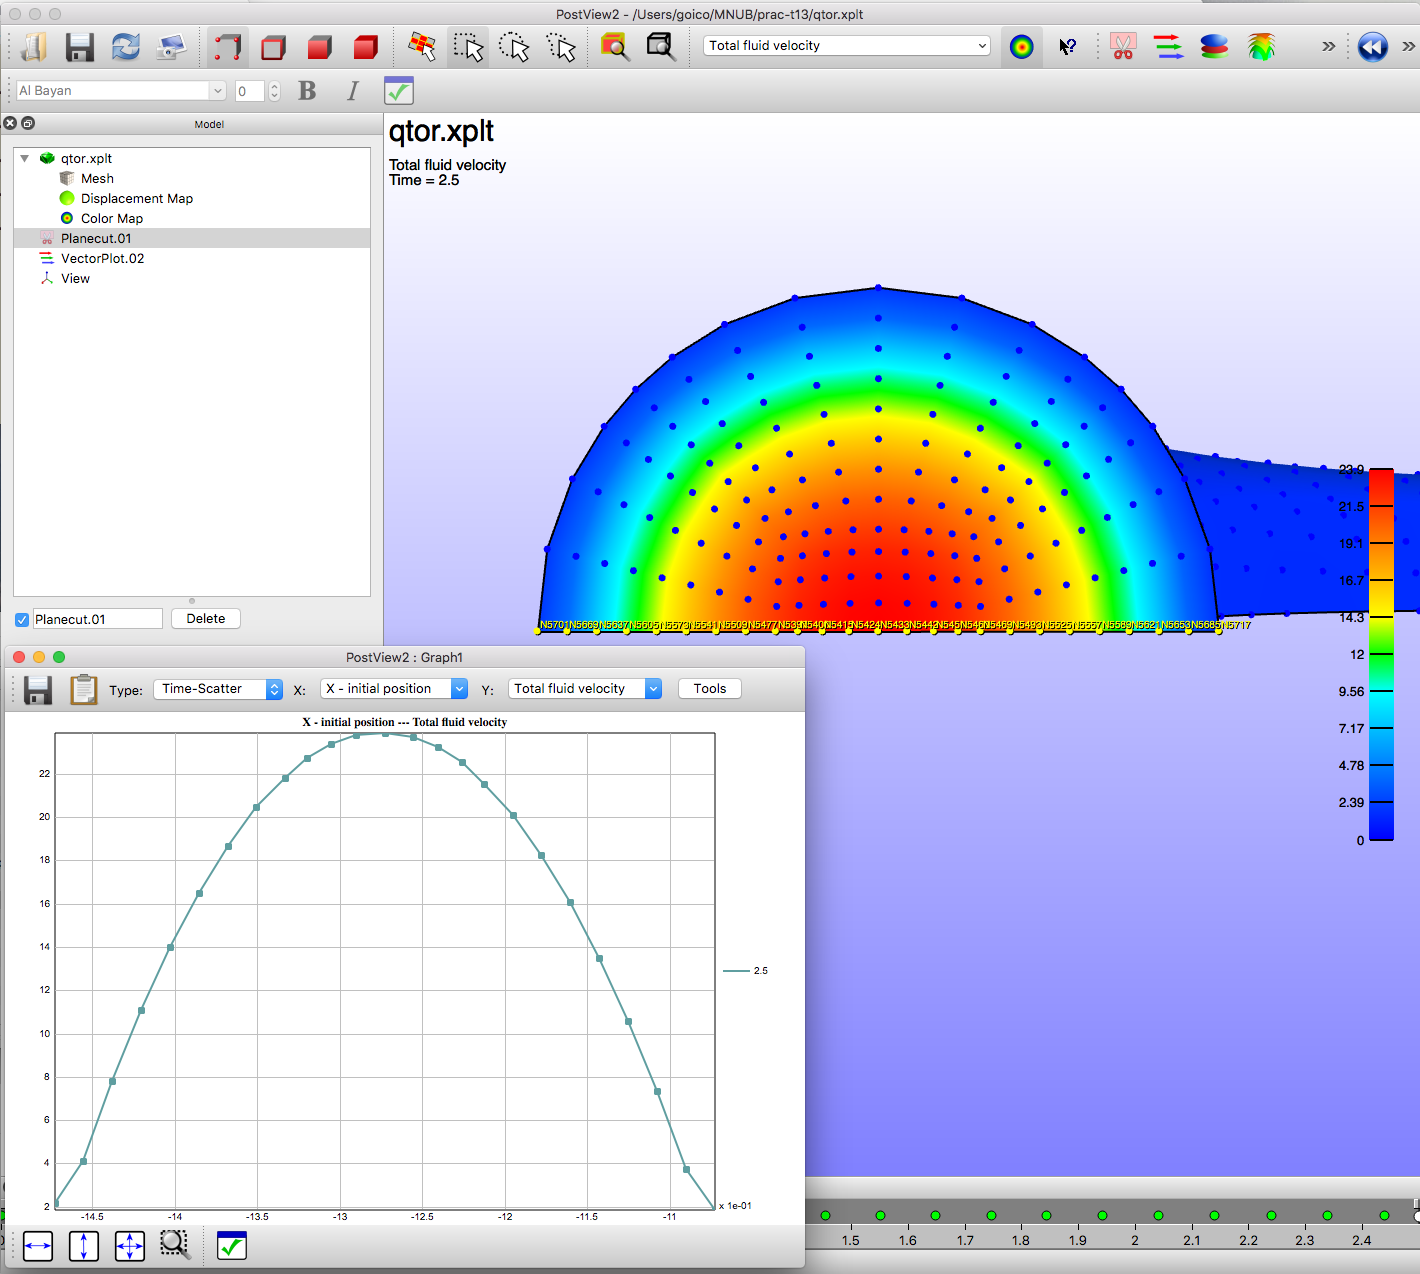
\includegraphics[width=0.5\linewidth]{figuras_4/14_post-profile-in.png}
\caption{Selección de perfil de velocidades en la sección de entrada}
\label{fig:14_post-profile-in}
\end{figure}

\begin{figure}[!ht]
\centering
\includegraphics[width=0.6\linewidth]{figuras_4/qtor-vr_comp.eps}
\caption{Comparación de perfiles de velocidades de entrada y salida con el modelo teórico de Poiseuille}
\label{fig:qtor-vr_comp}
\end{figure}

\clearpage
\section{Tareas para entregar}
\label{sec:tareas}

Deberán obtenerse y presentarse los siguientes resultados:%, agrupándolos en un fichero comprimido \texttt{G}\emph{nn}\texttt{.zip}, siendo \emph{nn} el número del grupo, que se subirá al sitio moodle.
\begin{enumerate}
	\item
	Perfil de velocidades en un diámetro de la sección de salida del tubo recto (sección~\ref{sec:tuborecto}) en el instante final, mediante copia de pantalla del gráfico.
	\item
	Perfil de velocidades en un diámetro de la sección de salida del tubo curvo (sección~\ref{sec:tubocurvo}) en el instante final, mediante copia de pantalla del gráfico.
	%\item
	%Fichero de video (\texttt{.avi} o \texttt{.mov}) con animación del mapa coloreado de las velocidades del fluido para el tubo curvo.
\end{enumerate}